\section{Compiling diet information}

%\subsection{Processing diet data from EltonTraits \citep{Wilman2014} for mammals and birds, and from AmphiBIO \citep{Oliveira2017} for amphibians}
For mammals and birds, diet information was obtained from the EltonTraits database \citep{Wilman2014}. Before processing the data, the taxonomy was aligned to that of the trait datasets compiled in Chapter 2. Primary diet -- that is, the diet inferred from the combination of food items that represent more than 50\% of species consumption -- was directly available for birds, but not for mammals. For both classes, diet was described as the percent use of different food items (namely: invertebrates, vertebrates -- either ectotherms, endotherms, fish or unknown --, carrion, fruit, nectar, seed or other plant material). In order to have a consistent classification scheme across mammals and birds, I chose not to use the provided primary diet for birds, and instead I applied my own procedure to infer primary diet from recorded food items across birds and mammals. I first grouped the different vertebrate food items together with carrion to create a single `vertebrate' food item category. I then used the percent uses of the food items to infer primary diet, classifying species’ primary diet into the following categories: vertebrate eaters; invertebrate eaters; plant/seed eaters; fruit/nectar eaters; and omnivores [these categories are similar to those employed for birds' primary diet in EltonTraits]. When all food items had a percent use below (or equal to) 50\% percent, species were classified as omnivores. %When a single food item had a percent use strictly above 50\%, species were classified into the corresponding primary diet group.
 For each species, I calculated diet breadth as the number of consumed food items (regardless of the percent use of those items; I kept vertebrate food items grouped together in the calculation of diet breadth, such that I did not count carrion as a separate food item). %Trophic levels for birds were also inferred from the primary diet (with fruit/nectar and plant/seed eaters considered herbivores, invertebrates/vertebrate eaters considered carnivores, and the remaining species considered omnivores).


For amphibians, diet information was partly extracted from the AmphiBIO database \citep{Oliveira2017}, and partly compiled from the literature (see next paragraph). In AmphiBIO, diet information was recorded as the consumption of six food items (leaves, flowers, seeds, fruit, arthropods and vertebrates), but the percent use of these items was not recorded (only whether they were consumed or not). From AmphiBIO, I classified amphibians into the different diet categories, depending on the combinations of consumed food items (with species consuming both plant and animal matter classified as omnivores; species consuming both vertebrates and invertebrates also classified as omnivores; and species consuming plant or seed only, fruit or nectar only, vertebrates only or invertebrates only classified into the corresponding groups). 

%\subsection{Diet data complements for amphibians and reptiles}
To increase diet data coverage for amphibians, I used data compiled by Rhiannon Osborne-Tonner, collected during her MSci project at UCL. Rhiannon Osborne-Tonner collected data from published papers and from the grey literature, targeting species occurring in the PREDICTS database (which I used for inferring land-use responses). Using these data, I was able to supplement my datasets with diet information for an additional 108 amphibians from 26 published sources (all found to be invertebrate eaters; see below for the list of sources). For reptiles, there was no readily available diet information (except for trophic level information, see Chapter 2). Thus, I used diet data compiled by Rhiannon Osborne-Tonner, collected from the literature, again specifically targeting reptiles occurring in the PREDICTS database. I was thus able to add diet information for 239 reptiles. Finally, I calculated diet breadth across amphibians and reptiles from the recorded food items. The diet data compiled by Rhiannon Osborne-Tonner are available at:
\url{https://figshare.com/articles/Reptile_Diet_csv/12024309} (DOI: 10.6084/m9.figshare.12024309.v1) and
\url{https://figshare.com/articles/Untitled_Item/12024312} (DOI: 10.6084/m9.figshare.12024312.v4).

\subsubsection*{Complementary data sources for amphibians}

\begin{itemize}
\item Aguilar-López \& Pineda (2013). An exotic species of earthworm preyed by \textit{Craugastor rhodopis}. Herpetology Notes, 6, 335-336.
\item Arroyo, S. B., Serrano-Cardozo, V. H., \& Ramírez-Pinilla, M. P. (2008). Diet, microhabitat and time of activity in a Pristimantis (Anura, Strabomantidae) assemblage. Phyllomedusa: Journal of Herpetology, 7(2), 109-119.         
\item Loc Barragán, J. A. \& Woolrich, G. (2016). Smilisca baudinii. Diet. Mesoamerican Herpetology, 3(3).
\item Berry, P. Y., \& Bullock, J. A. (1962). The Food of the Common Malayan Toad, \textit{Bufo melanostictus} Schneider. Copeia, 1962(4), 736–741. 
\item Blommers-Schlösser, R. M. A. (1975). A unique case of mating behaviour in a Malagasy tree frog, Gephyromantis liber (Peracca, 1893), with observations on the larval development (Amphibia, Ranidae). Beaufortia, 23(296), 15–25.
\item Cappo, M. (1986). Frogs as predators of organisms of aquatic origin in the Magela Creek System, Northern Territory. MSc thesis. Dept of Zoology, University of Adelaide. https://hdl.handle.net/2440/110846.
\item Costello, J.M. (2013). Differences in Morphology and Behavior in Green Frogs (\textit{Lithobates clamitans} from Urban and Rural Sites in New York and New Jersey. PhD thesis. City University of New York. 
\item Brito de Carvalho, C. \& Freitas, E. \& Faria, R. \& Batista, R. \& Batista, C. \& Coelho, W. \& Bocchiglieri, A. (2008). Natural history of \textit{Leptodactylus mystacinus} and \textit{Leptodactylus fuscus} (Anura: Leptodactylidae) in the Cerrado of Central Brazil. Biota Neotropica, 8. 
\item Batista, R. \& Brito de Carvalho, C. \& Freitas, E.B. \& Franco, S.C. \& Batista, C.C. \& Coelho, Welington \& Faria, Renato. (2011). Diet of \textit{Rhinella schneideri} (Werner, 1894) (Anura: Bufonidae) in the Cerrado, Central Brazil. Herpetology Notes, 4:17-21. 
\item Fonseca-Pérez, K. A., Molina, C., \& Tárano, Z. (2017). Diet of Dendropsophus microcephalus and Scarthyla vigilans (Anura: Hylidae) at a locality in north-western Venezuela with notes on microhabitat occupation. Papéis Avulsos De Zoologia, 57(7), 93-104.
\item García-R, J.C. \& Posso-Gómez, C. E. \& Cárdenas-Henao, H. (2015). Diet of direct-developing frogs (Anura: Craugastoridae: Pristimantis) from the Andes of western Colombia. Acta Biológica Colombiana, 20:79-87. 
\item Zumbado-Ulato, H. \& Acosta-Chaves, V. (2012). \textit{Cochranella granulosa} (Granular glass frog) feeding behaviour. Herpetological review.
\item Yap, C.H. \& Jafaar, I. (2012). Feeding analysis of \textit{Hylarana cf. labialis}, \textit{Leptobrchiun hendricksoni}, and \textit{Occidozyga laevis} (Amphibia: Anura) from a lowland dipterocarp forest in Kedah, Malaysia. Herpetological Review, 43(1).
\item Schwenk, K. (2000). Feeding: Form, function and evolution in tetrapod vertebrates. Academic Press.
\item Sabagh, L.T., Ferreira V.L., \& Rocha C.F. (2010). Living together, sometimes feeding in a similar way: the case of the syntopic hylid frogs Hypsiboas raniceps and Scinax acuminatus (Anura: Hylidae) in the Pantanal of Miranda, Mato Grosso do Sul State, Brazil. Brazilian Journal of Biology, 70(4):955-9.
\item Luría-Manzano R. \& Ramírez-Bautista A. (2017). Diet comparison between rainforest and cave populations of \textit{Craugastor alfredi} (Anura: Craugastoridae): does diet vary in contrasting habitats? Journal of Natural History, 51:39-40, 2345-2354.
\item Martínez-Coronel, M. \& Pérez-Gutiérrez, M. (2011). Diet composition of \textit{Craugastor lineatus} (Anura: Craugastoridae) of Chiapas, Mexico. Acta Zoológica Mexicana 27(2):215-230. 
\item McAlister, W. H. (1963). Evidence of mild toxicity in the saliva of the hognose snake (Heterodon). Herpetologica, 19:132-137.
\item Moreno-Barbosa, S. \& Hoyos, J. (2014). Ontogeny of the diet in Anurans (Amphibia) collected at La Vieja river basin in the deparmento of Quindio (Colombia). Caldasia, 36 (365-372).
\item Piatti, L. \& Souza, F. (2011). Diet and resource partitioning among anurans in irrigated rice fields in Pantanal, Brazil. Brazilian journal of biology, 71 (653-61).
\item Savini, C. O. K., Chuang, M. F., \& Ishida, C. (2004). Diet Selection in the Green Paddy Frog (\textit{Rana erythraea}). International field biology course 2004.
\item Simon, M. P., \& Toft, C. A. (1991). Diet Specialization in Small Vertebrates: Mite-Eating in Frogs. Oikos, 61(2):263–278. 
\item Sugai, J.L.M.M., Terra, J.S., \& Ferreira, V.L. (2012): Diet of \textit{Leptodactylus fuscus}
(Amphibia: Anura: Leptodactylidae) in the Pantanal of Miranda river, Brazil. Biota Neotropica, 12: 99-104.
\item Toft, C. A. (1981). Feeding Ecology of Panamanian Litter Anurans: Patterns in Diet and Foraging Mode. Journal of Herpetology, 15(2):139–144. 
\item Vences, M., Glaw, F. \& Zapp, C.(1999). Stomach content analysis in Malagasy frogs of the genera \textit{Tomopterna}, \textit{Aglyptodactylus}, \textit{Boophis} and \textit{Mantidactylus}. Herpetozoa, 11(3/4):109-116.
\item Yap, C.H. \& Jaafar, I. (2011). Stomach Content Analysis of Tropical Forest Toads \textit{Ingerophrynus parvus} and \textit{Phrynoides aspera} (ANURA : BUFONIDAE) from Kedah, Malaysia. Taxonomist and Ecologist Conference 2011.
\end{itemize}

\subsubsection*{Complementary data sources for reptiles}

The 148 sources are listed in the dataset available from \url{https://figshare.com/articles/Reptile_Diet_csv/12024309} (DOI: 10.6084/m9.figshare.12024309.v1).

\newpage
\section{Imputing missing trait values}

\subsection{Trait data coverage}
%% trait coverage across all vertebrates
\begin{figure}[h!]
\centering
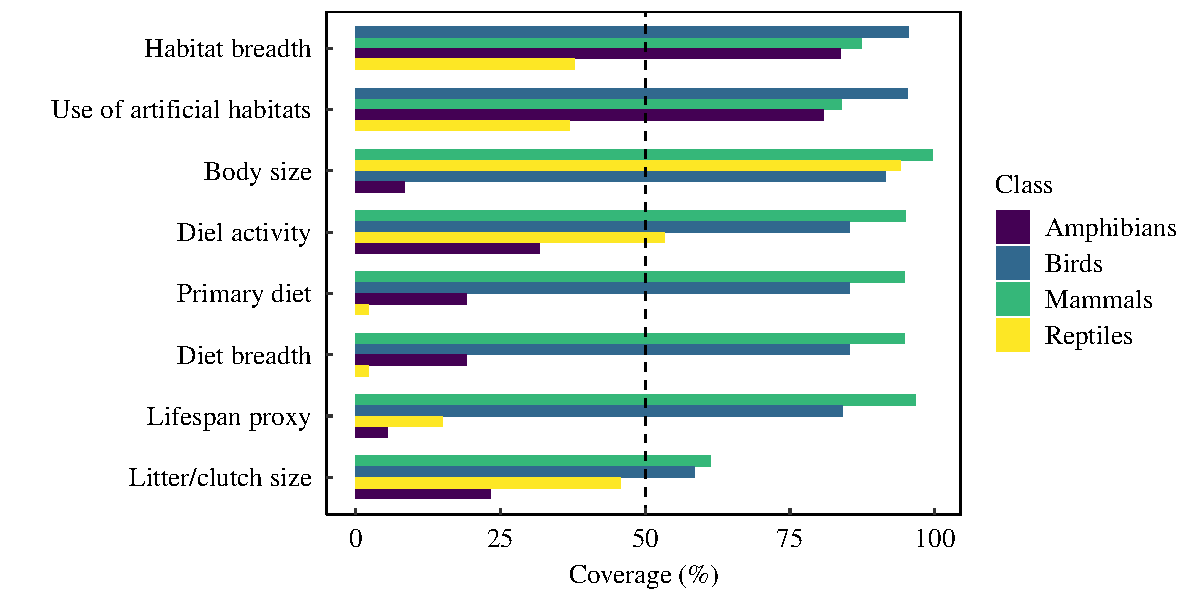
\includegraphics[scale=0.8]{Supporting/Chapter4/Figures/Coverage_all_species}
\caption[Trait coverage across vertebrate classes, including coverage for diet information]{\textbf{Trait coverage, including coverage for diet information, calculated as the proportion of species for which trait values are not missing}. The dashed line represents 50\% coverage.}
\label{SI_4_fig1}
\end{figure}

\subsection{Phylogenetic signal in traits}
%% phylogenetic signal
I measured the phylogenetic signal in traits using Pagel's $\lambda$ (for continuous traits) and Borges' $\delta$ (for categorical traits). I found evidence of phylogenetic conservatism in all traits.

\begin{table}[h!]
\renewcommand{\baselinestretch}{1}
\renewcommand{\arraystretch}{1.2}
\begin{center}\fontsize{9}{11}\selectfont
\caption[Phylogenetic signal in continuous and categorical traits]{\textbf{Phylogenetic signal in continuous and categorical traits.} BM: body mass; BL: body length; GL: generation length; MA: age at sexual maturity; ML: maximum longevity; L: longevity; LCS: litter/clutch size; HB: habitat breadth; DA: diel activity; UA: use of artificial habitats. Continuous traits were log-10 transformed to improve normality before estimating Pagel’s $\lambda$ – except for habitat breadth and diet breadth which were square-rooted. A star indicates a significant signal (P<0.05 for the log-likelihood ratio test in the case of $\lambda$; and a significant difference from the simulated null distribution of $\delta$ for categorical traits). ‘NA’ indicates traits that were not considered for a given class. %All traits showed significant phylogenetic signal, with signals for BM, BL, L, GL, MA and LCS being particularly strong (above 0.8) across the four classes. 
}
\label{SI_4_Table1}  
\begin{tabular}{l|c|c|c|c|c|c|c|c|c|c|c|c|}
\cline{2-13}
                                          & \multicolumn{9}{c|}{\textbf{Pagel's $\lambda$}}                                                                       & \multicolumn{3}{c|}{\textbf{Borges' $\delta$}} \\ \hline
\multicolumn{1}{|c|}{\textbf{Class}}      & \textbf{BM} & \textbf{BL} & \textbf{GL} & \textbf{MA} & \textbf{ML} & \textbf{L} & \textbf{LCS} & \textbf{HB} & \textbf{Diet breadth} & \textbf{Diet} &  \textbf{DA} & \textbf{UA} \\ \hline
\multicolumn{1}{|l|}{\textbf{Amphibians}} & 0.98*       & 0.94*       & NA          & 0.85*       & 0.82*       & NA         & 0.93*        & 0.99*    & 0.61*  & 3.4*         &  3.4*        & 4.5*        \\ %\hline
\multicolumn{1}{|l|}{\textbf{Birds}}      & 0.99*       & NA          & 0.97*       & NA          & NA          & NA         & 0.95*        & 0.60*   &  0.72*   & 6.4*         & 32e3*     & 1.8*        \\ %\hline
\multicolumn{1}{|l|}{\textbf{Mammals}}    & 0.99*       & NA          & 0.97        & NA          & NA          & NA         & 0.99         & 0.71    &  0.99*  & 26*         & 52*      & 1.3*        \\ %\hline
\multicolumn{1}{|l|}{\textbf{Reptiles}}   & 1.0*        & NA          & NA          & NA          & 0.94*       & 0.98*      & 1.0*         & 0.52*    & 0.84*  & 2.2*        & 6.4*     & 1.4*        \\ \hline
\end{tabular}
\end{center}
\end{table}

\begin{comment}
\begin{itemize}
\item Amphibians: $\delta$=3.424413, p-value = 4.768e-07
\item Birds: $\delta$=6.466144, p-value =  0.007813
\item Mammals: $\delta$=, p-value =  
\item Reptiles: $\delta$=2.248912, p-value = 2.91e-11
\end{itemize}
\end{comment}


\subsection{Implementation of missing value imputations}
I imputed missing trait values using random forest algorithms, as implemented in R with `missForest' \citep{Stekhoven2012, Stekhoven2016}. Phylogenetic relationships were included as additional predictors in the form of phylogenetic eigenvectors \citep{DinizFilho2012}, extracted from the phylogenies using the PVR package \citep{Santos2018}. I used class-specific phylogenetic trees from \url{https://zenodo.org/record/3690867#.Xyc5wyhKhPZ} for mammals (Phylacine 1.2; Faurby et al. (2018, 2020)); and from \url{https://data.vertlife.org/} for amphibians (Jetz \& Pyron 2018), birds (Jetz et al. 2012) and squamates (Tonini et al. 2016). For each class, I used a consensus tree obtained with the TreeAnnotator programme of the BEAST software (Bouckaert et al. 2014), from an available distribution of 1000 trees. 

Following \citet{Penone2014}, I included the first ten phylogenetic eigenvectors as additional predictors of missing trait values in each class. As not all species were represented in the phylogenies, I also added taxonomic order as a predictor for all species. All traits in Table \ref{SI_4_Table1} were included in the imputations. Habitat \& diet breadth were considered as categorical variables for the imputations (and so, discretised), in order to ensure that only integer estimates were obtained from the imputations for these traits. Tuning parameters of `missforest' were set to ten maximum iterations and to one hundred trees grown in each forest.

%% distribution of traits before and after imputations


\subsection{Imputation error}

%% plot for imputation errors
\begin{figure}[h!]
\centering
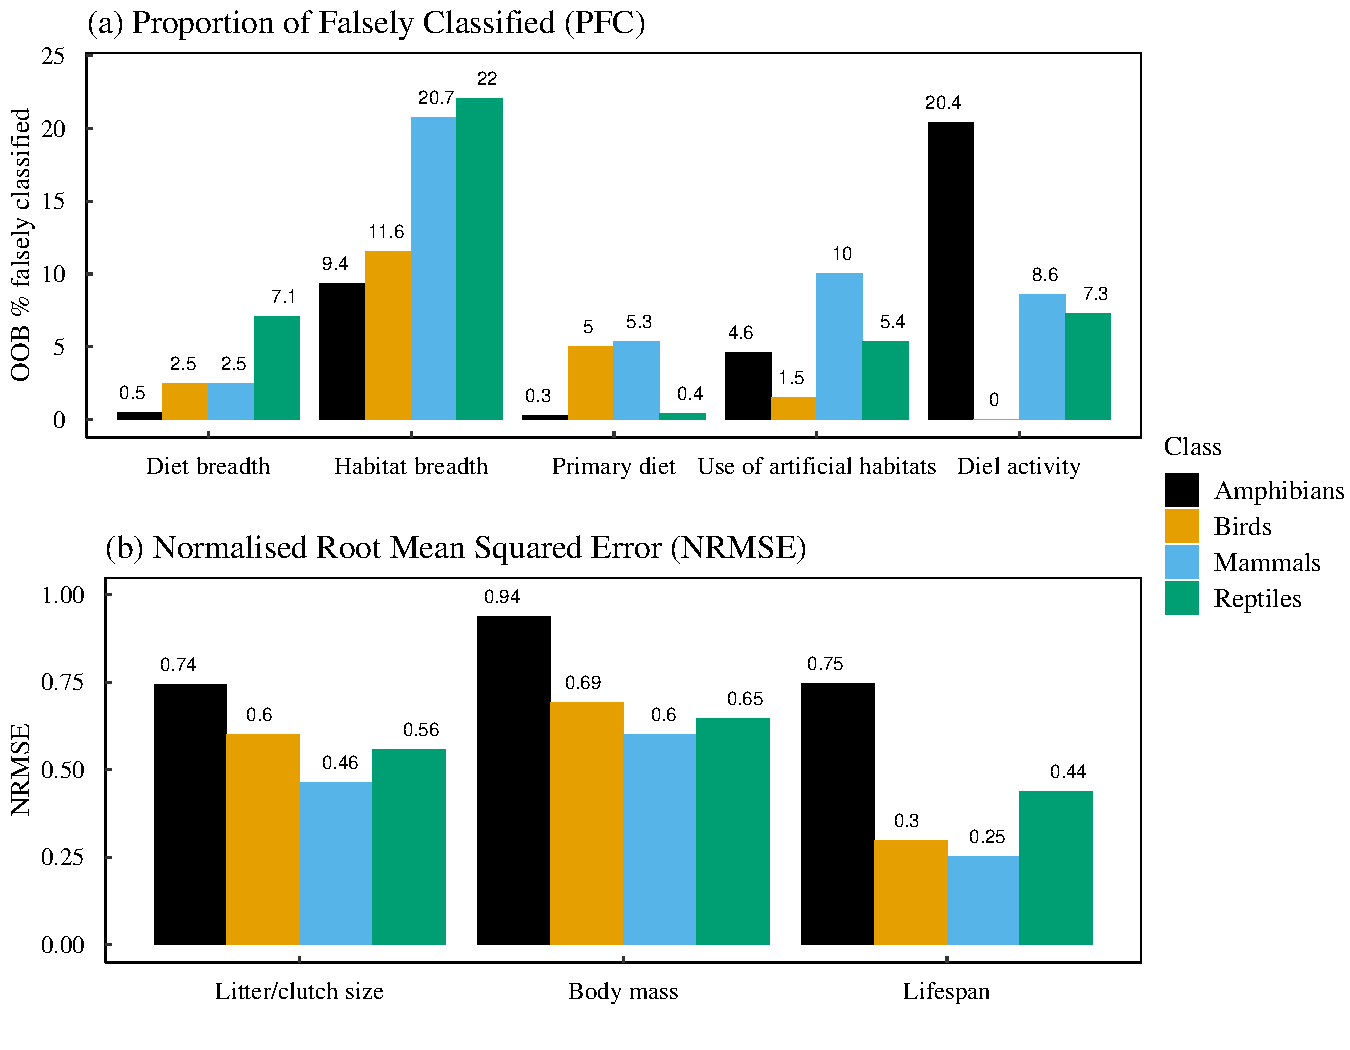
\includegraphics[scale=0.7]{Supporting/Chapter4/Figures/Imputation_errors}
\caption[Out-of-bag estimation of imputation errors for the traits included in the analyses]{\textbf{Out-of-bag estimation of imputation errors for the traits included in the analyses.} \textbf{(a)} For the categorical traits, I show the proportion of falsely classified traits (`PFC', out-of-bag estimates); \textbf{(b)} For the continuous traits, I calculate the normalised root-mean-squared error (NRMSE), from the out-of-bag mean square error that I divide by the standard deviation of the known trait distribution. The lower the NRMSE, the lower the imputation error, with values close to 0 indicating lower imputation error and values close to 1 tending to indicate higher imputation error.} 
% ($\text{NRMSE}=\frac{\sqrt{\text{mean}(\text{X}_{\text{true}}-\text{X}_{\text{imputed}})^2}}{\text{standard deviation (X}_\text{true})}$, where X represents values of a trait distribution).}
\label{SI_4_Figure2}
\end{figure}

%NRMSE=$\sqrt{\text{mean}(\text{X}_{\text{true}}-\text{X}_{\text{imputed}})^2}/SD_{X}$


\begin{comment}
%% plot for imputation congruence

\begin{figure}[h!]
\centering
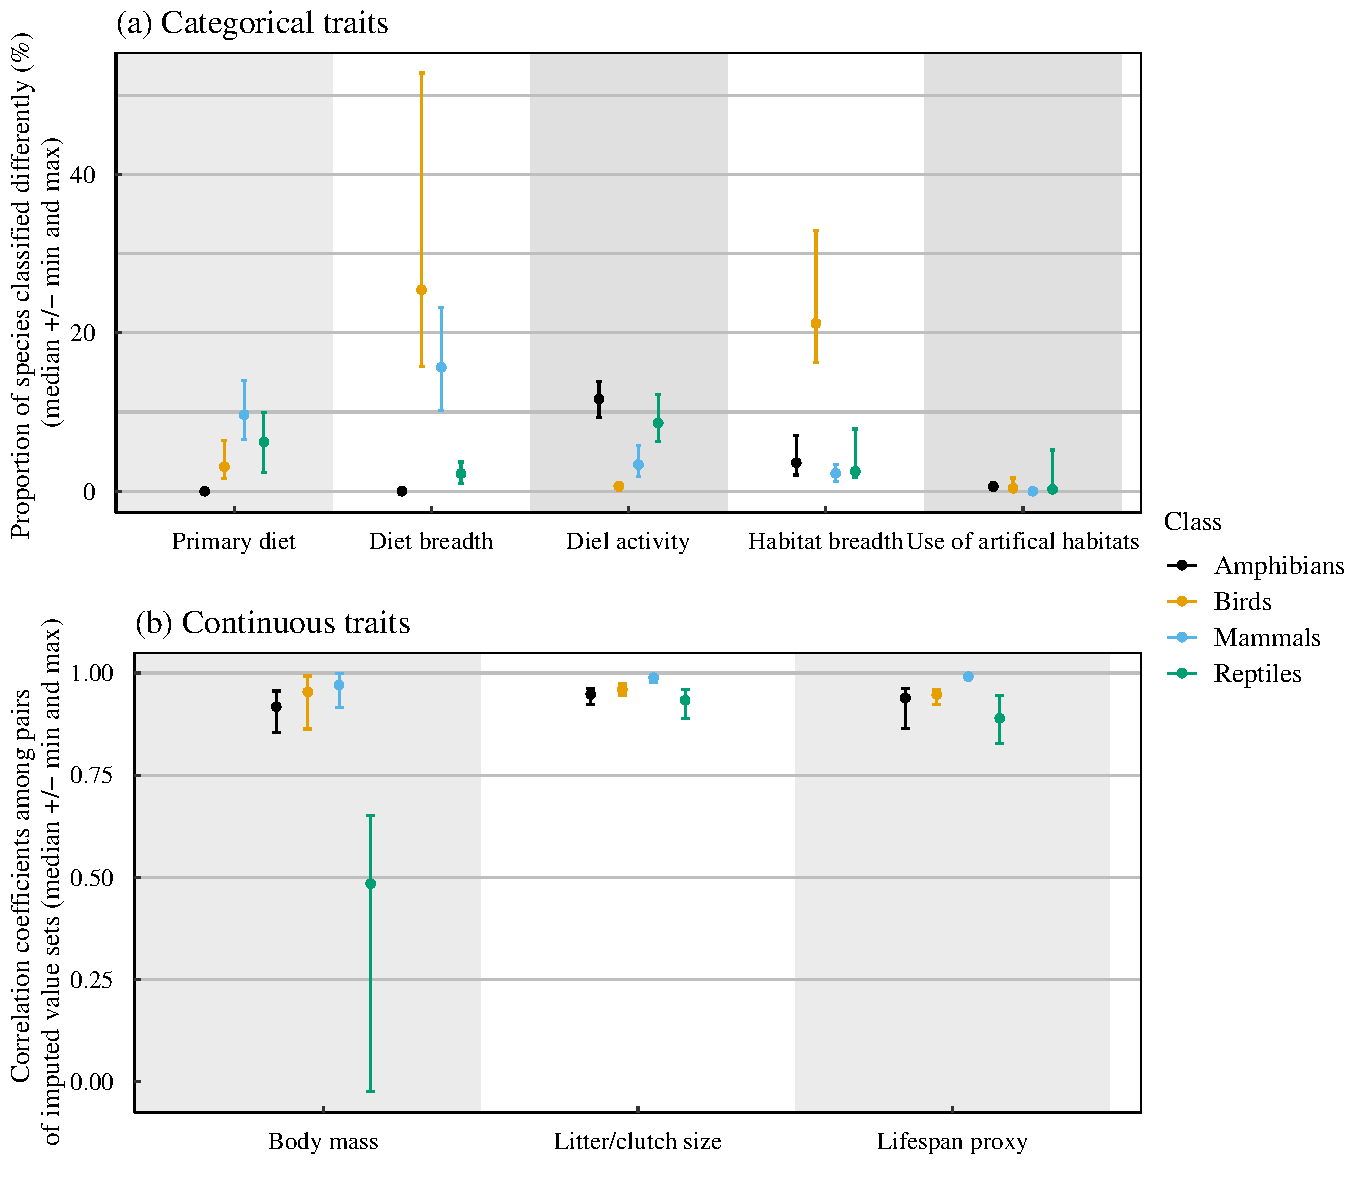
\includegraphics[scale=0.7]{Supporting/Chapter4/Figures/Imputation_congruence}
\caption[Imputation congruence among eight independent sets of imputed traits]{\textbf{Imputation congruence among eight independent sets of imputed traits.} \textbf{(a)} For the categorical traits, I show the median and the range of the proportion of species for which different imputation rounds yielded different imputed values. The proportion of species for which the estimated values were different between two imputed datasets was obtained for each pair of imputed sets (by obtaining pairwise comparisons among the eights sets of imputed datasets). \textbf{(b)} For the continuous traits, I show the range and median of the correlation coefficients among pairs of imputed sets, for each trait.}
\label{SI_4_Figure3}
\end{figure}

\end{comment}

\clearpage

\section{Land-use types in PREDICTS and sample sizes (number of sampled sites across classes)}

%% table PREDICTS land-use types
%% TABLE OF DEFINITION OF LAND USES
\begin{table}[h!]
\renewcommand{\baselinestretch}{1}
\renewcommand{\arraystretch}{1.2}
\begin{center}\fontsize{9}{11}\selectfont
\caption[Land-use categories in the PREDICTS database]{\textbf{Land-use categories in the PREDICTS database.} See \citet{Hudson2014, Hudson2017} for more details.} 
\label{SI_4_Table2}  
\begin{tabular}{|l|l|}
\hline
\multicolumn{1}{|c|}{\textbf{Land-use category}}        & \multicolumn{1}{c|}{\textbf{Definition}}                                                                                                                                                                                                                                                    \\ \hline
Primary vegetation                                      & \begin{tabular}[c]{@{}l@{}}Native vegetation, undisturbed since its establishment under current climatic conditions.\\ No known alterations due to human activities or to extreme natural events.\end{tabular}                                                           \\ \hline
Mature secondary vegetation                             & \begin{tabular}[c]{@{}l@{}}Vegetation recovering after complete destruction of primary vegetation\\ \& where succession is near complete – the structure approaches that of primary vegetation.  \end{tabular}               \\ \hline
\multicolumn{1}{|c|}{Intermediate secondary vegetation} & \begin{tabular}[c]{@{}l@{}}Vegetation recovering after complete destruction of primary vegetation \\at a mid-successional stage.\end{tabular}                                                                   \\ \hline
Young secondary vegetation                              & \begin{tabular}[c]{@{}l@{}}Vegetation recovering after complete destruction of primary vegetation \\at an early successional stage.\end{tabular}                                                         \\ \hline
Plantation forest                                       & \begin{tabular}[c]{@{}l@{}}Previously cleared areas planted with crop trees or shrubs \\grown and harvested for human consumption or for commercial purposes \\(includes wood, fruit, oil, biofuel, rubber, etc). \end{tabular}                                                             \\ \hline
Pasture                                                 & \begin{tabular}[c]{@{}l@{}}Areas grazed by livestock, permanently or regularly. \\Can be improved through cultivation techniques.\end{tabular}                                                                                                                                            \\ \hline
Cropland                                                & \begin{tabular}[c]{@{}l@{}}Previously cleared areas planted with herbaceous crops\\ and harvested for human or animal consumption\\ (including animal feed and crops used in the food industry),\\ or for commercial purposes (e.g., crops grown for the textile industry).\end{tabular} \\ \hline
Urban                                                   & \begin{tabular}[c]{@{}l@{}}Previously cleared areas built up by humans. \\Vegetation is managed for civic or personal purposes.\end{tabular}                                                                                                                                  \\ \hline
\end{tabular}
\end{center}
\end{table}



%% figure sample sizes
\begin{figure}[h!]
\centering
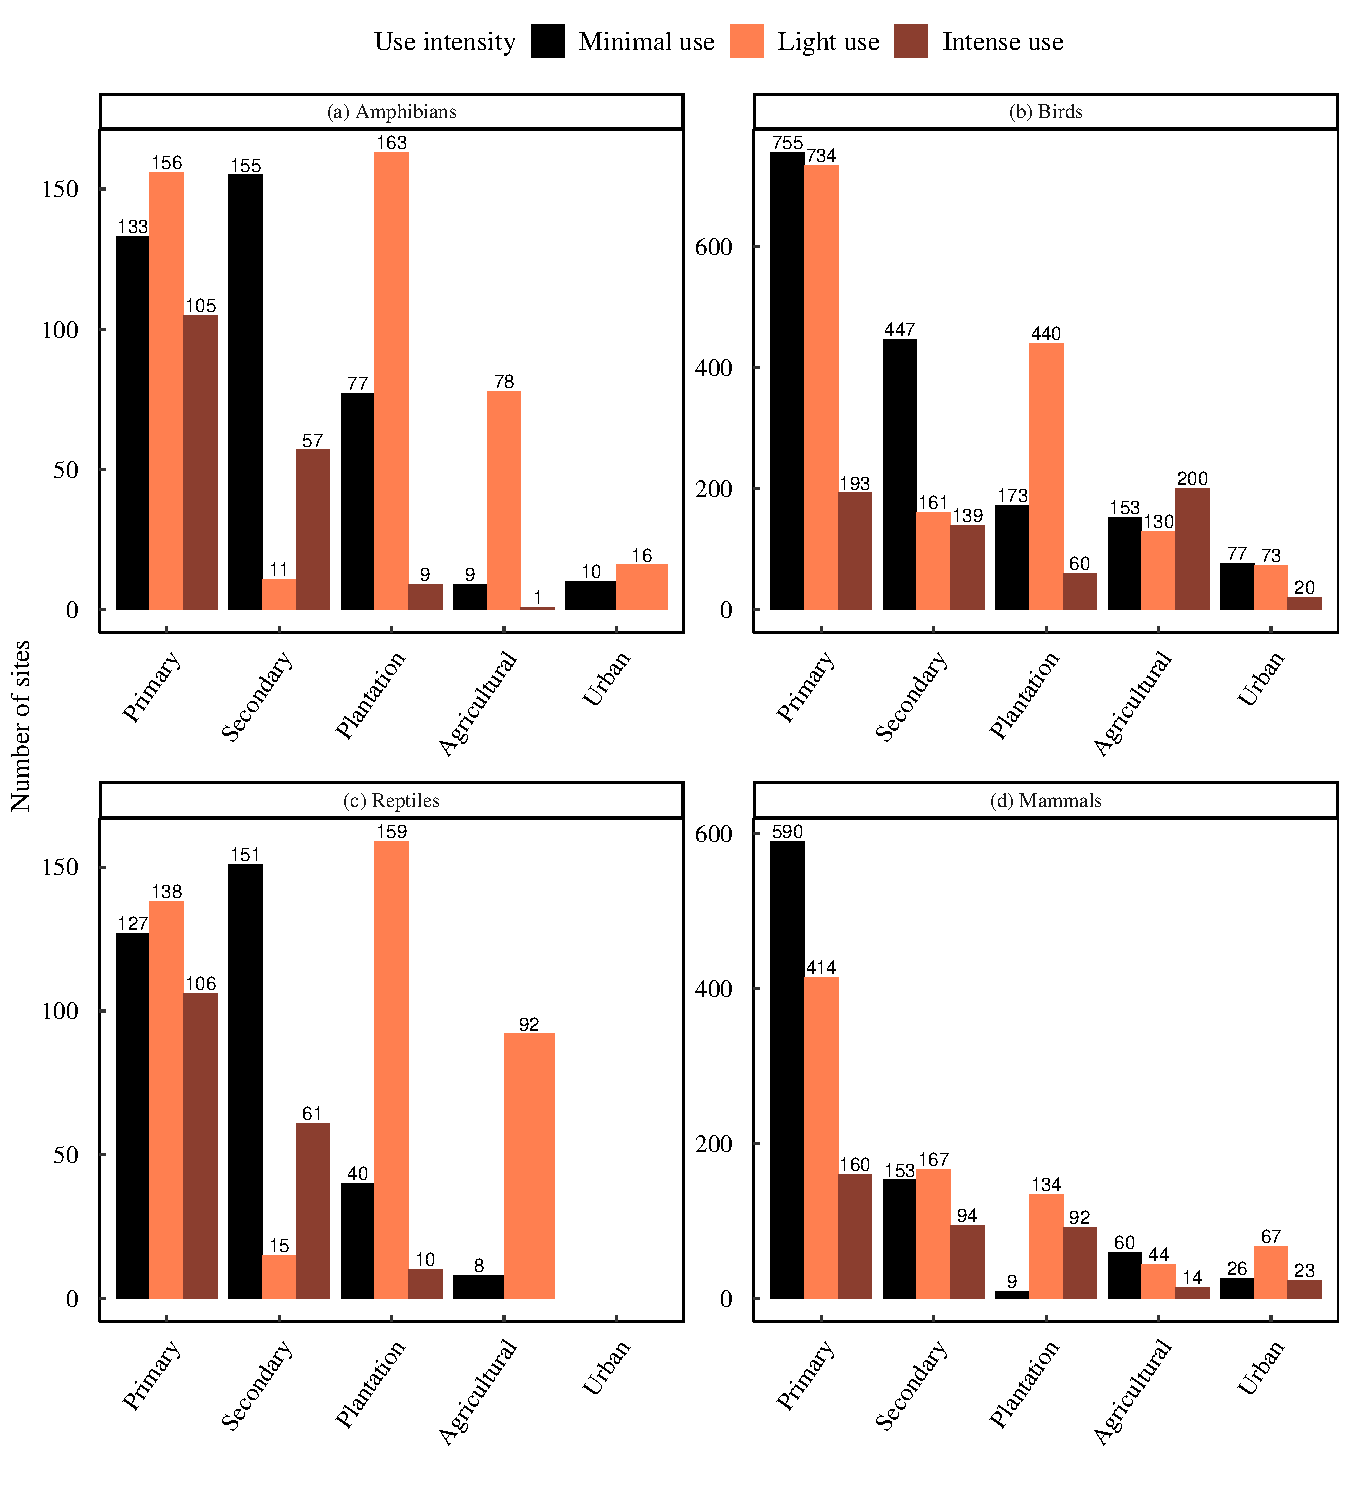
\includegraphics[scale=0.7]{Supporting/Chapter4/Figures/Sample_size_figure}
\caption[Sample sizes (number of PREDICTS sites) for the different land-use types, in each class]{\textbf{Sample sizes (number of PREDICTS sites) for the different land-use types, in each class.}}
\label{SI_4_Figure4}
\end{figure}

\clearpage
\section{Land-use responses: multicollinearity checks among the models' explanatory variables}

%% Amphibians, with primary diet
\begin{table}[!h] 
\renewcommand{\baselinestretch}{1}
\renewcommand{\arraystretch}{1}
\begin{center}\fontsize{9}{11}\selectfont 
  \caption[Land-use responses: Generalised Variance Inflation Factors (amphibians, with diet)]{\textbf{Generalised Variance Inflation Factors among the candidate explanatory variables for the mixed-effects model fitted across amphibians, \textit{prior to the exclusion of diet}}. The model aimed at investigating the effects of land use, land-use intensity and the species-level ecological characteristics on species occurrence probability.} 
  \label{SI_4_Table3} 
\begin{tabular}{@{\extracolsep{5pt}} cc} 
\\[-1.8ex]\hline 
\hline \\[-1.8ex] 
 Predictor & GVIF \\ 
\hline \\[-1.8ex] 
Diel activity & $1.7$ \\ 
Lifespan proxy (log$_{10}$) & $1.8$ \\ 
Specialisation & $1.8$ \\ 
Range area (log$_{10}$) & $2.0$ \\ 
Body mass (log$_{10}$) & $2.0$ \\ 
Land use & $2.0$ \\ 
Litter/clutch size (log$_{10}$) & $2.5$ \\ 
Land-use intensity & $2.6$ \\ 
Habitat breadth (square-root) & $3.2$ \\ 
Diet breadth (square-root) & $22.8$ \\ 
Primary diet & $23.6$ \\ 
\hline \\[-1.8ex] 
\end{tabular} 
\end{center}
\end{table}  

\vspace{-0.5cm}
%% Amphibians, without primary diet
\begin{table}[h!] 
\renewcommand{\baselinestretch}{1}
\renewcommand{\arraystretch}{1}
\begin{center}\fontsize{9}{11}\selectfont
    \caption[Land-use responses: Generalised Variance Inflation Factors (amphibians, without diet)]{\textbf{Generalised Variance Inflation Factors among the explanatory variables for the mixed-effects model fitted across amphibians \textit{(after the exclusion of diet)}}, looking at the effects of land use, land-use intensity and the species-level ecological characteristics on species occurrence probability.}  
  \label{SI_4_Table4} 
\begin{tabular}{@{\extracolsep{5pt}} cc} 
\\[-1.8ex]\hline 
\hline \\[-1.8ex] 
Predictor & GVIF \\ 
\hline \\[-1.8ex] 
Diel activity & $1.6$ \\ 
Diet breadth (square-root) & $1.7$ \\ 
Lifespan proxy (log$_{10}$) & $1.8$ \\ 
Specialisation & $1.8$ \\ 
Range area (log$_{10}$) & $1.9$ \\ 
Land use & $2.0$ \\ 
Body mass (log$_{10}$) & $2.0$ \\ 
Litter/clutch size (log$_{10}$) & $2.4$ \\ 
Land-use intensity & $2.6$ \\ 
Habitat breadth (square-root) & $3.1$ \\ 
\hline \\[-1.8ex] 
\end{tabular} 
\end{center}
\end{table} 

\vspace{-0.5cm}
%% birds
\begin{table}[!h] 
\renewcommand{\baselinestretch}{1}
\renewcommand{\arraystretch}{1}
\begin{center}\fontsize{9}{11}\selectfont
  \caption[Land-use responses: Generalised Variance Inflation Factors (birds)]{\textbf{Generalised Variance Inflation Factors among the explanatory variables for the mixed-effects model fitted across birds}, looking at the effects of land use, land-use intensity and the species-level ecological characteristics on species occurrence probability.} 
  \label{SI_4_Table5} 
\begin{tabular}{@{\extracolsep{5pt}} cc} 
\\[-1.8ex]\hline 
\hline \\[-1.8ex] 
Predictor & GVIF \\ 
\hline \\[-1.8ex] 
Diel activity & $1.1$ \\ 
Land use & $1.2$ \\ 
Land-use intensity & $1.2$ \\ 
Litter/clutch size (log$_{10}$) & $1.3$ \\ 
Range area (log$_{10}$) & $1.4$ \\ 
Diet breadth (square-root) & $1.5$ \\ 
Specialisation & $1.6$ \\ 
Lifespan proxy (log$_{10}$) & $1.7$ \\ 
Habitat breadth (square-root) & $1.8$ \\ 
Body mass (log$_{10}$) & $1.9$ \\ 
Primary diet & $2.3$ \\ 
\hline \\[-1.8ex] 
\end{tabular}
\end{center} 
\end{table} 

\vspace{-0.5cm}
%% mammals
\begin{table}[!h] 
\renewcommand{\baselinestretch}{1}
\renewcommand{\arraystretch}{1}
\begin{center}\fontsize{9}{11}\selectfont 
  \caption[Land-use responses: Generalised Variance Inflation Factors (mammals)]{\textbf{Generalised Variance Inflation Factors among the explanatory variables for the mixed-effects model fitted across mammals}, looking at the effects of land use, land-use intensity and the species-level ecological characteristics on species occurrence probability.}  
  \label{SI_4_Table6} 
\begin{tabular}{@{\extracolsep{5pt}} cc} 
\\[-1.8ex]\hline 
\hline \\[-1.8ex] 
Predictor & GVIF \\ 
\hline \\[-1.8ex] 
Diel activity & $1.2$ \\ 
Range area (log$_{10}$)& $1.2$ \\ 
Specialisation & $1.4$ \\ 
Land-use intensity & $1.4$ \\ 
Diet breadth (square-root) & $1.7$ \\ 
Land use & $1.8$ \\ 
Habitat breadth (square-root) & $1.8$ \\ 
Litter/clutch size (log$_{10}$) & $2.7$ \\ 
Body mass (log$_{10}$) & $3.0$ \\ 
Lifespan proxy (log$_{10}$) & $3.4$ \\ 
Primary diet & $4.4$ \\ 
\hline \\[-1.8ex] 
\end{tabular} 
\end{center}
\end{table} 

\vspace{-0.5cm}
%% reptiles, with primary diet
\begin{table}[!h]
\renewcommand{\baselinestretch}{1}
\renewcommand{\arraystretch}{1}
\begin{center}\fontsize{9}{11}\selectfont 
%  \caption{Generalised Variance Inflation Factors among species-level predictors for the mixed-effects model fitted across reptiles, prior to the exclusion of primary diet.} 
  \caption[Land-use responses: Generalised Variance Inflation Factors (reptiles, with diet)]{\textbf{Generalised Variance Inflation Factors among the candidate explanatory variables for the mixed-effects model fitted across reptiles, \textit{prior to the exclusion of diet}}. The model aimed at investigating the effects of land use, land-use intensity and the species-level ecological characteristics on species occurrence probability.} 
  \label{SI_4_Table7} 
\begin{tabular}{@{\extracolsep{5pt}} cc} 
\\[-1.8ex]\hline 
\hline \\[-1.8ex] 
 Predictor & GVIF \\ 
\hline \\[-1.8ex] 
Diel activity & $1.1$ \\ 
Specialisation & $1.3$ \\ 
Range area (log$_{10}$) & $1.3$ \\ 
Habitat breadth (square-root) & $1.6$ \\ 
Lifespan proxy (log$_{10}$) & $1.9$ \\ 
Litter/clutch size (log$_{10}$) & $2.8$ \\ 
Land use & $3.2$ \\ 
land-use intensity & $3.5$ \\ 
Body mass (log$_{10}$) & $3.9$ \\ 
Diet breadth (square-root) & $5.8$ \\ 
Primary diet & $9.9$ \\ 
\hline \\[-1.8ex] 
\end{tabular} 
\end{center}
\end{table} 

%% reptiles, excluding primary diet
\begin{table}[!h] 
\renewcommand{\baselinestretch}{1}
\renewcommand{\arraystretch}{1}
\begin{center}\fontsize{9}{11}\selectfont 
  %\caption{Generalised Variance Inflation Factors among species-level predictors for the mixed-effects model fitted across reptiles, after the exclusion of primary diet.} 
    \caption[Land-use responses: Generalised Variance Inflation Factors (reptiles, without diet)]{\textbf{Generalised Variance Inflation Factors among the explanatory variables for the mixed-effects model fitted across reptiles \textit{(after the exclusion of diet)}}, looking at the effects of land use, land-use intensity and the species-level ecological characteristics on species occurrence probability.}  
  \label{SI_4_Table8} 
\begin{tabular}{@{\extracolsep{5pt}} cc} 
\\[-1.8ex]\hline 
\hline \\[-1.8ex] 
 Predictor & GVIF \\ 
\hline \\[-1.8ex] 
Diel activity & $1.1$ \\ 
Diet breadth (square-root) & $1.2$ \\ 
Specialisation & $1.2$ \\ 
Range area (log$_{10}$)& $1.3$ \\ 
Habitat breadth (square-root) & $1.6$ \\ 
Lifespan proxy (log$_{10}$) & $1.9$ \\ 
Litter/clutch size (log$_{10}$) & $2.7$ \\ 
Land use & $3.2$ \\ 
Body mass (log$_{10}$) & $3.2$ \\ 
Land-use intensity & $3.4$ \\ 
\hline \\[-1.8ex] 
\end{tabular} 
\end{center}
\end{table} 

\clearpage

\section{Implementing Climate-niche Factor Analysis across terrestrial vertebrates}

\subsection{Historical climate data: groups of intercorrelated variables}
%trim = left lower right upper
\begin{figure}[h!]
\centering
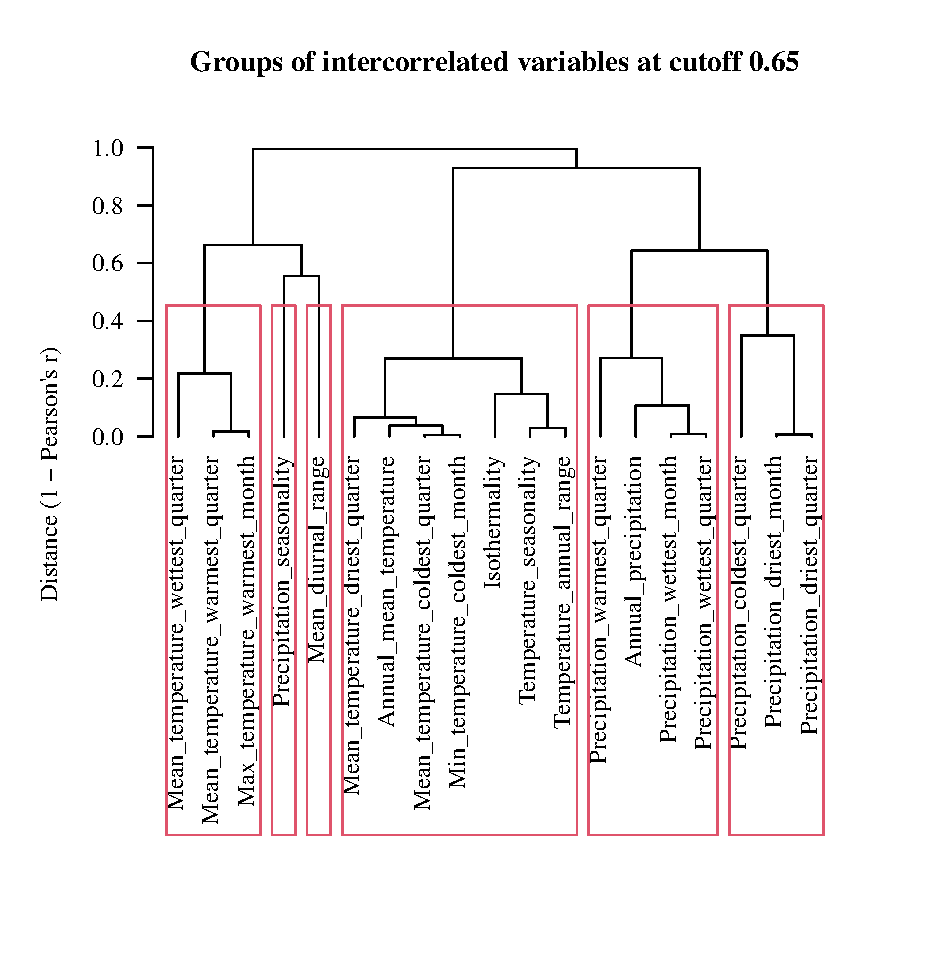
\includegraphics[scale=0.9, trim={0 1.75cm 0 2cm},clip]{Supporting/Chapter4/Figures/ClimVars_groups2}
\caption[Groups of intercorrelated climatic variables using a cutoff of 0.65 for Pearson's correlation coefficient]{\textbf{Groups of intercorrelated climatic variables using a cutoff of 0.65 for Pearson's correlation coefficient}, obtained using the `removeCollinearity' R function (`virtualspecies' package, \citet{virtualspecies}). Variables figuring in the same red boxes were correlated with Pearson's correlation coefficient > 0.65.}
\label{SI_4_Figure5}
\end{figure}


\subsection{CENFA estimation and resolution}
I estimated climate-change sensitivity across terrestrial vertebrates with the CENFA framework using three different resolutions for the species distribution files and the climatic variables: 50 km$^2$, 10 km$^2$ and 5 km$^2$. The finer the resolution, the better the species' distribution is likely to be captured, particularly for narrow-ranging species (Figure \ref{SI_4_Figure6}). When working with coarser resolutions, the actual geographical distribution of a narrow-ranging species might be overestimated (Figure \ref{SI_4_Figure6}), such that the climatic niche breadth of the species might also be overestimated; consequently, its climate-change sensitivity may be underestimated. However, finer resolutions are more computationally demanding, which can be limiting when working across several thousand species. 

Thus, I looked for a resolution that provided the best compromise between accuracy of sensitivity estimation and computational load (Figure \ref{SI_4_Figure7}).
% With a resolution of 50 km$^2$, climate-change sensitivity tended to be overestimated for a larger number of narrow-ranging species than at 10 km$^2$ (Figure \ref{SI_4_Figure7}); and at 10 km$^2$, climate-change sensitivity tended to be overestimated for a larger number of narrow-ranging species than at 5 km$^2$ (Figure \ref{SI_4_Figure7}). 
%Below 5 km$^2$, I deemed the computational load not acceptable for a global estimation of climate-change sensitivity across terrestrial vertebrates.
Hence, I chose to work with a resolution of 5 km$^2$. At this resolution, there were still some narrow-ranging species for which sensitivity was likely overestimated (Figure \ref{SI_4_Figure7}). To prevent any impact of these species on the analyses, I removed species with the smallest geographical range areas, using a conservative threshold of 100 km$^2$ for geographical range area (Figure \ref{SI_4_Figure7}).

\vspace{0.5cm}
\begin{figure}[h!]
\centering
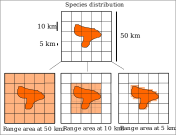
\includegraphics[scale=0.6]{Supporting/Chapter4/Figures/ResolutionConcept.png}
\caption[Possible impact of resolution on estimated geographical range area]{\textbf{Possible impact of resolution on estimated geographical range area}. I represent a virtual distribution for a species (orange shape). The species distribution is more accurately captured at finer resolutions (e.g., 5 km$^2$) than at coarser resolutions (e.g., 10 km$^2$ or 50 km$^2$). A possible consequence is that coarser resolutions can tend to disproportionally overestimate the geographical range area of narrow-ranging species, because the aggregation of grid cells where the species is found to be present can artificially augment the amount of occupied area at coarser resolutions, and relatively more so if the species is narrow-ranging.}
\label{SI_4_Figure6}
\end{figure}
  
\clearpage


\begin{comment}
\vspace{-4cm}
\begin{figure}[h!]
\centering
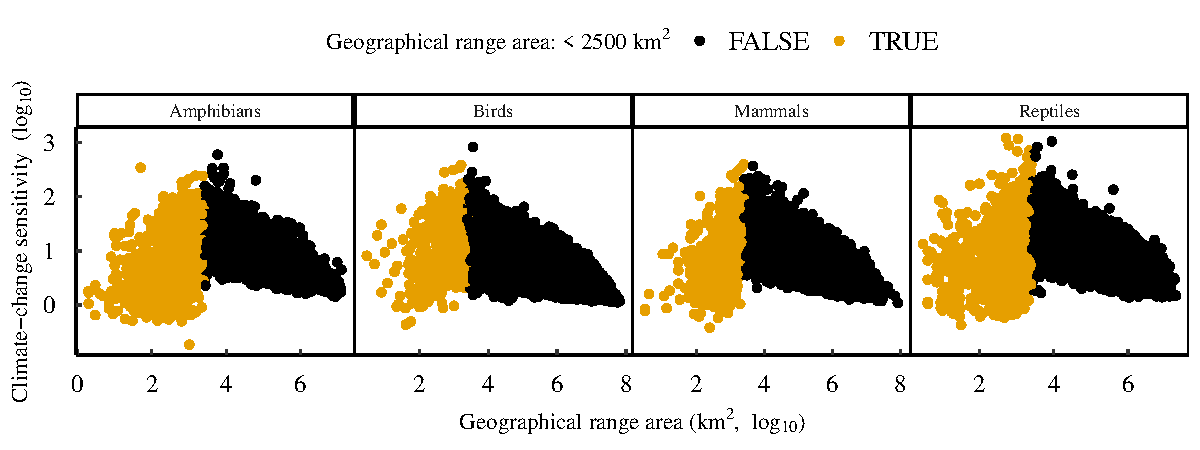
\includegraphics[scale=0.8]{Supporting/Chapter4/Figures/CENFA_50km}
\caption[]{\textbf{Climate-change sensitivity estimations using a resolution of 50 km$^2$ against geographical range area (estimated at 1 km$^2$).} I highlight the species whose range area is below 2,500 km$^2$, that is, the species whose distribution intersect one grid cell only. Climate-change sensitivity was estimated using the CENFA framework \citep{Rinnan2019}.}
\label{CENFA50}
\end{figure}

\vspace{-2cm}
\begin{figure}[h!]
\centering
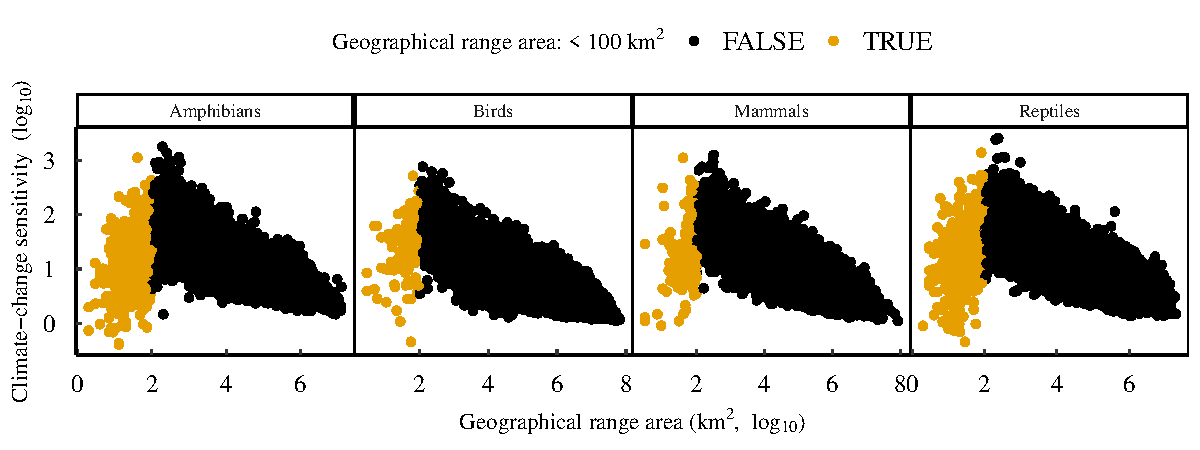
\includegraphics[scale=0.8]{Supporting/Chapter4/Figures/CENFA_10km}
\caption[]{\textbf{Climate-change sensitivity estimations using a resolution of 10 km$^2$ against geographical range area (estimated at 1 km$^2$).} I highlight the species whose range area is below 100 km$^2$, that is, the species whose distribution intersect one grid cell only. Climate-change sensitivity was estimated using the CENFA framework \citep{Rinnan2019}.}
\label{CENFA10}
\end{figure}

\vspace{-2cm}
\begin{figure}[h!]
\centering
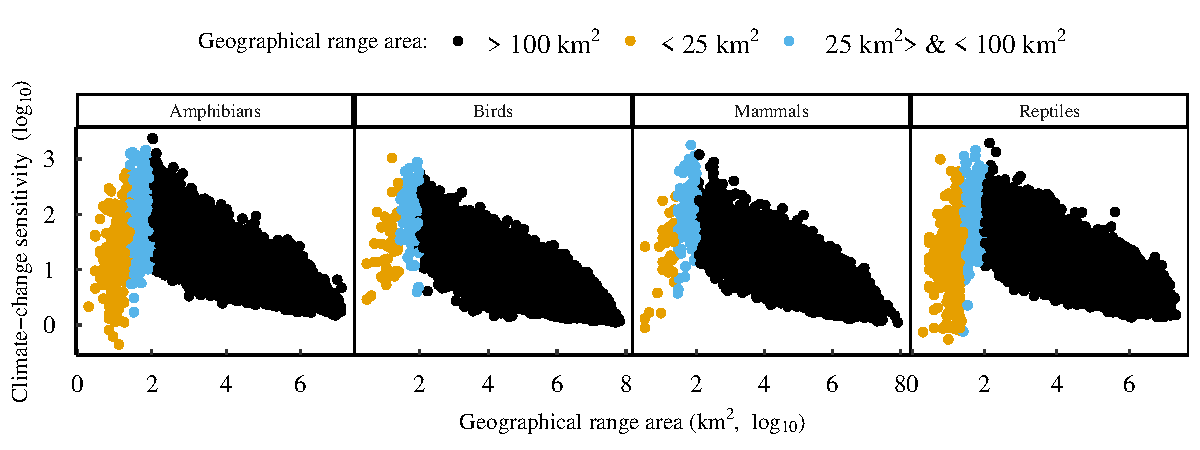
\includegraphics[scale=0.8]{Supporting/Chapter4/Figures/CENFA_5km}
\caption[]{\textbf{Climate-change sensitivity estimations at 5 km$^2$ against geographical range area (estimated at 1 km$^2$).} I highlight the species whose range area is above 100 km$^2$, that is, the species whose distribution intersect up to four grid cells. Climate-change sensitivity was estimated using the CENFA framework \citep{Rinnan2019}.}
\label{CENFA5}
\end{figure}

\end{comment}

\begin{figure}[h!]
\centering
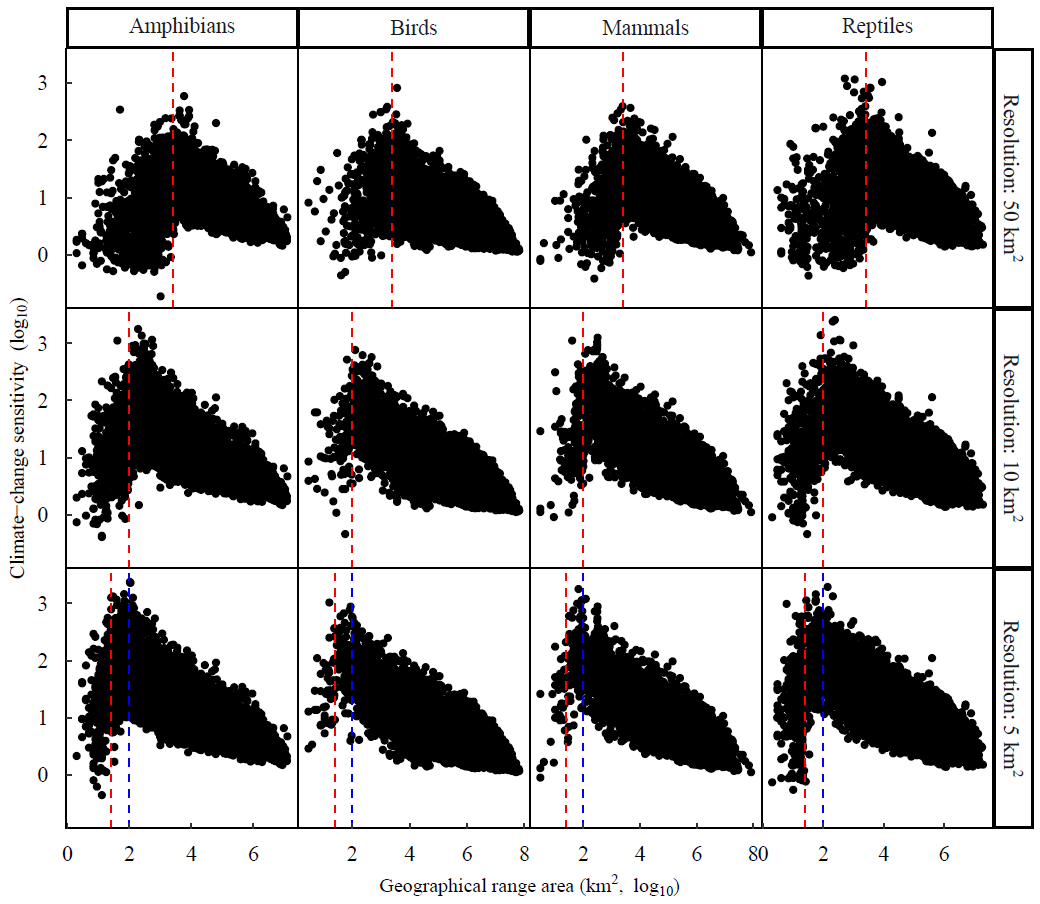
\includegraphics[scale=0.6]{Supporting/Chapter4/Figures/CENFA_allres.png}
\caption[Estimated climate-change sensitivity estimations at three different resolutions]{\textbf{Estimated climate-change sensitivity estimations at three different resolutions (50 km$^2$, 10 km$^2$ and 5 km$^2$) against geographical range area (estimated at 1 km$^2$).} With the red dashed lines, I highlight the range areas that correspond to the surface area of one grid cell (\textit{i.e.}, 2,500 km$^2$, 100 km$^2$ and 25 km$^2$ respectively). Climate-change sensitivity was estimated using the CENFA framework \citep{Rinnan2019}. I chose to work at a resolution of 5 km$^2$ and I excluded species whose range area was $\leq$100km$^2$ (blue dashed line), that is, species whose distribution could intersect up to four grid cells at a resolution of 5 km$^2$.}
\label{SI_4_Figure7}
\end{figure}

\clearpage

\section{Climate-change sensitivity models: multicollinearity checks among models' explanatory variables}

%% Amphibians, with diet breadth

\begin{table}[!h]
\renewcommand{\baselinestretch}{1}
\renewcommand{\arraystretch}{1}
\begin{center}\fontsize{9}{11}\selectfont 
    \caption[PGLS models: Generalised Variance Inflation Factors (amphibians, with diet breadth)]{\textbf{Generalised Variance Inflation Factors among the candidate explanatory variables for the phylogenetic least-square regression fitted across amphibians, \textit{prior to the exclusion of diet breadth}}. The model aimed at investigating the association between the species-level ecological characteristics and species climate-change sensitivity.} 
  \label{SI_4_Table9} 
\begin{tabular}{@{\extracolsep{5pt}} cc} 
\\[-1.8ex]\hline 
\hline \\[-1.8ex] 
 Predictor & GVIF \\ 
\hline \\[-1.8ex] 
Diel activity & $1.1$ \\ 
Lifespan proxy (log$_{10}$) & $1.2$ \\ 
Range area (log$_{10}$) & $1.3$ \\ 
Body mass (log$_{10}$) & $1.4$ \\ 
Litter/clutch size (log$_{10}$) & $1.5$ \\ 
Specialisation & $1.6$ \\ 
Habitat breadth (square-root) & $1.9$ \\ 
Primary diet & $17.1$ \\ 
Diet breadth (square-root) & $17.1$ \\ 
\hline \\[-1.8ex] 
\end{tabular} 
\end{center}
\end{table} 

%% Amphibians, without diet breadth
\begin{table}[!h] 
\renewcommand{\baselinestretch}{1}
\renewcommand{\arraystretch}{1}
\begin{center}\fontsize{9}{11}\selectfont 
    \caption[PGLS models: Generalised Variance Inflation Factors (amphibians, without diet breadth)]{\textbf{Generalised Variance Inflation Factors among the explanatory variables for the phylogenetic least-square regression fitted across amphibians, \textit{after excluding diet breadth}}. The model aimed at investigating the association between the species-level ecological characteristics and species climate-change sensitivity.} 
  \label{SI_4_Table10} 
\begin{tabular}{@{\extracolsep{5pt}} cc} 
\\[-1.8ex]\hline 
\hline \\[-1.8ex] 
 Predictor & GVIF \\ 
\hline \\[-1.8ex] 
Diel activity & $1.1$ \\ 
Primary diet & $1.1$ \\ 
Lifespan proxy (log$_{10}$) & $1.2$ \\ 
Range area (log$_{10}$) & $1.3$ \\ 
Body mass (log$_{10}$) & $1.4$ \\ 
Litter/clutch size (log$_{10}$) & $1.5$ \\ 
Specialisation & $1.6$ \\ 
Habitat breadth (square-root) & $1.9$ \\ 
\hline \\[-1.8ex] 
\end{tabular} 
\end{center}
\end{table} 


%% Birds
\begin{table}[!h] 
\renewcommand{\baselinestretch}{1}
\renewcommand{\arraystretch}{1}
\begin{center}\fontsize{9}{11}\selectfont
    \caption[PGLS models: Generalised Variance Inflation Factors (birds)]{\textbf{Generalised Variance Inflation Factors among the explanatory variables for the phylogenetic least-square regression fitted across birds.} The model aimed at investigating the association between the species-level ecological characteristics and species climate-change sensitivity.} 
  \label{SI_4_Table11} 
\begin{tabular}{@{\extracolsep{5pt}} cc} 
\\[-1.8ex]\hline 
\hline \\[-1.8ex] 
Predictor & GVIF \\ 
\hline \\[-1.8ex] 
Diel activity & $1.1$ \\ 
Range area (log$_{10}$) & $1.2$ \\ 
Litter/clutch size (log$_{10}$) & $1.3$ \\ 
Diet breadth (square-root) & $1.5$ \\ 
Specialisation & $1.6$ \\ 
Habitat breadth (square-root) & $1.8$ \\ 
Lifespan proxy (log$_{10}$) & $1.9$ \\ 
Body mass (log$_{10}$)& $2.0$ \\ 
Primary diet & $2.1$ \\ 
\hline \\[-1.8ex] 
\end{tabular} 
\end{center}
\end{table} 

%% Mammals
\begin{table}[!h] 
\renewcommand{\baselinestretch}{1}
\renewcommand{\arraystretch}{1}
\begin{center}\fontsize{9}{11}\selectfont 
    \caption[PGLS models: Generalised Variance Inflation Factors (mammals)]{\textbf{Generalised Variance Inflation Factors among the explanatory variables for the phylogenetic least-square regression fitted across mammals.} The model aimed at investigating the association between the species-level ecological characteristics and species climate-change sensitivity.} 
  \label{SI_4_Table12} 
\begin{tabular}{@{\extracolsep{5pt}} cc} 
\\[-1.8ex]\hline 
\hline \\[-1.8ex] 
Predictor & GVIF \\ 
\hline \\[-1.8ex] 
Range area (log$_{10}$) & $1.2$ \\ 
Diel activity & $1.3$ \\ 
Specialisation & $1.3$ \\ 
Habitat breadth (square-root) & $1.5$ \\ 
Diet breadth (square-root) & $1.6$ \\ 
Body mass(log$_{10}$) & $2.3$ \\ 
Litter/clutch size (log$_{10}$) & $2.4$ \\ 
Primary diet & $2.7$ \\ 
Lifespan proxy (log$_{10}$) & $3.0$ \\ 
\hline \\[-1.8ex] 
\end{tabular} 
\end{center}
\end{table} 

%% Reptiles
\begin{table}[!h] 
\renewcommand{\baselinestretch}{1}
\renewcommand{\arraystretch}{1}
\begin{center}\fontsize{9}{11}\selectfont 
    \caption[PGLS models: Generalised Variance Inflation Factors (reptiles)]{\textbf{Generalised Variance Inflation Factors among the explanatory variables for the phylogenetic least-square regression fitted across reptiles.} The model aimed at investigating the association between the species-level ecological characteristics and species climate-change sensitivity.}
  \label{SI_4_Table13} 
\begin{tabular}{@{\extracolsep{5pt}} cc} 
\\[-1.8ex]\hline 
\hline \\[-1.8ex] 
 Predictor & GVIF \\ 
\hline \\[-1.8ex] 
Diel activity & $1.1$ \\ 
Range area(log$_{10}$) & $1.2$ \\ 
Specialisation & $1.4$ \\ 
Habitat breadth (square-root)& $1.5$ \\ 
Lifespan proxy (log$_{10}$) & $1.6$ \\ 
Litter/clutch size (log$_{10}$) & $2.0$ \\ 
Body mass (log$_{10}$) & $2.9$ \\ 
Diet breadth (square-root) & $2.9$ \\ 
Primary diet & $3.6$ \\ 
\hline \\[-1.8ex] 
\end{tabular} 
\end{center}
\end{table} 

%%%%%%%%%%%%%%%%%%%%%%%%%%%%%%%%
\clearpage

\begin{comment}
\section{Land-use responses: estimated effects from full (all-predictor) models}

%% categorical traits - effects
\begin{figure}[h!]
\centering
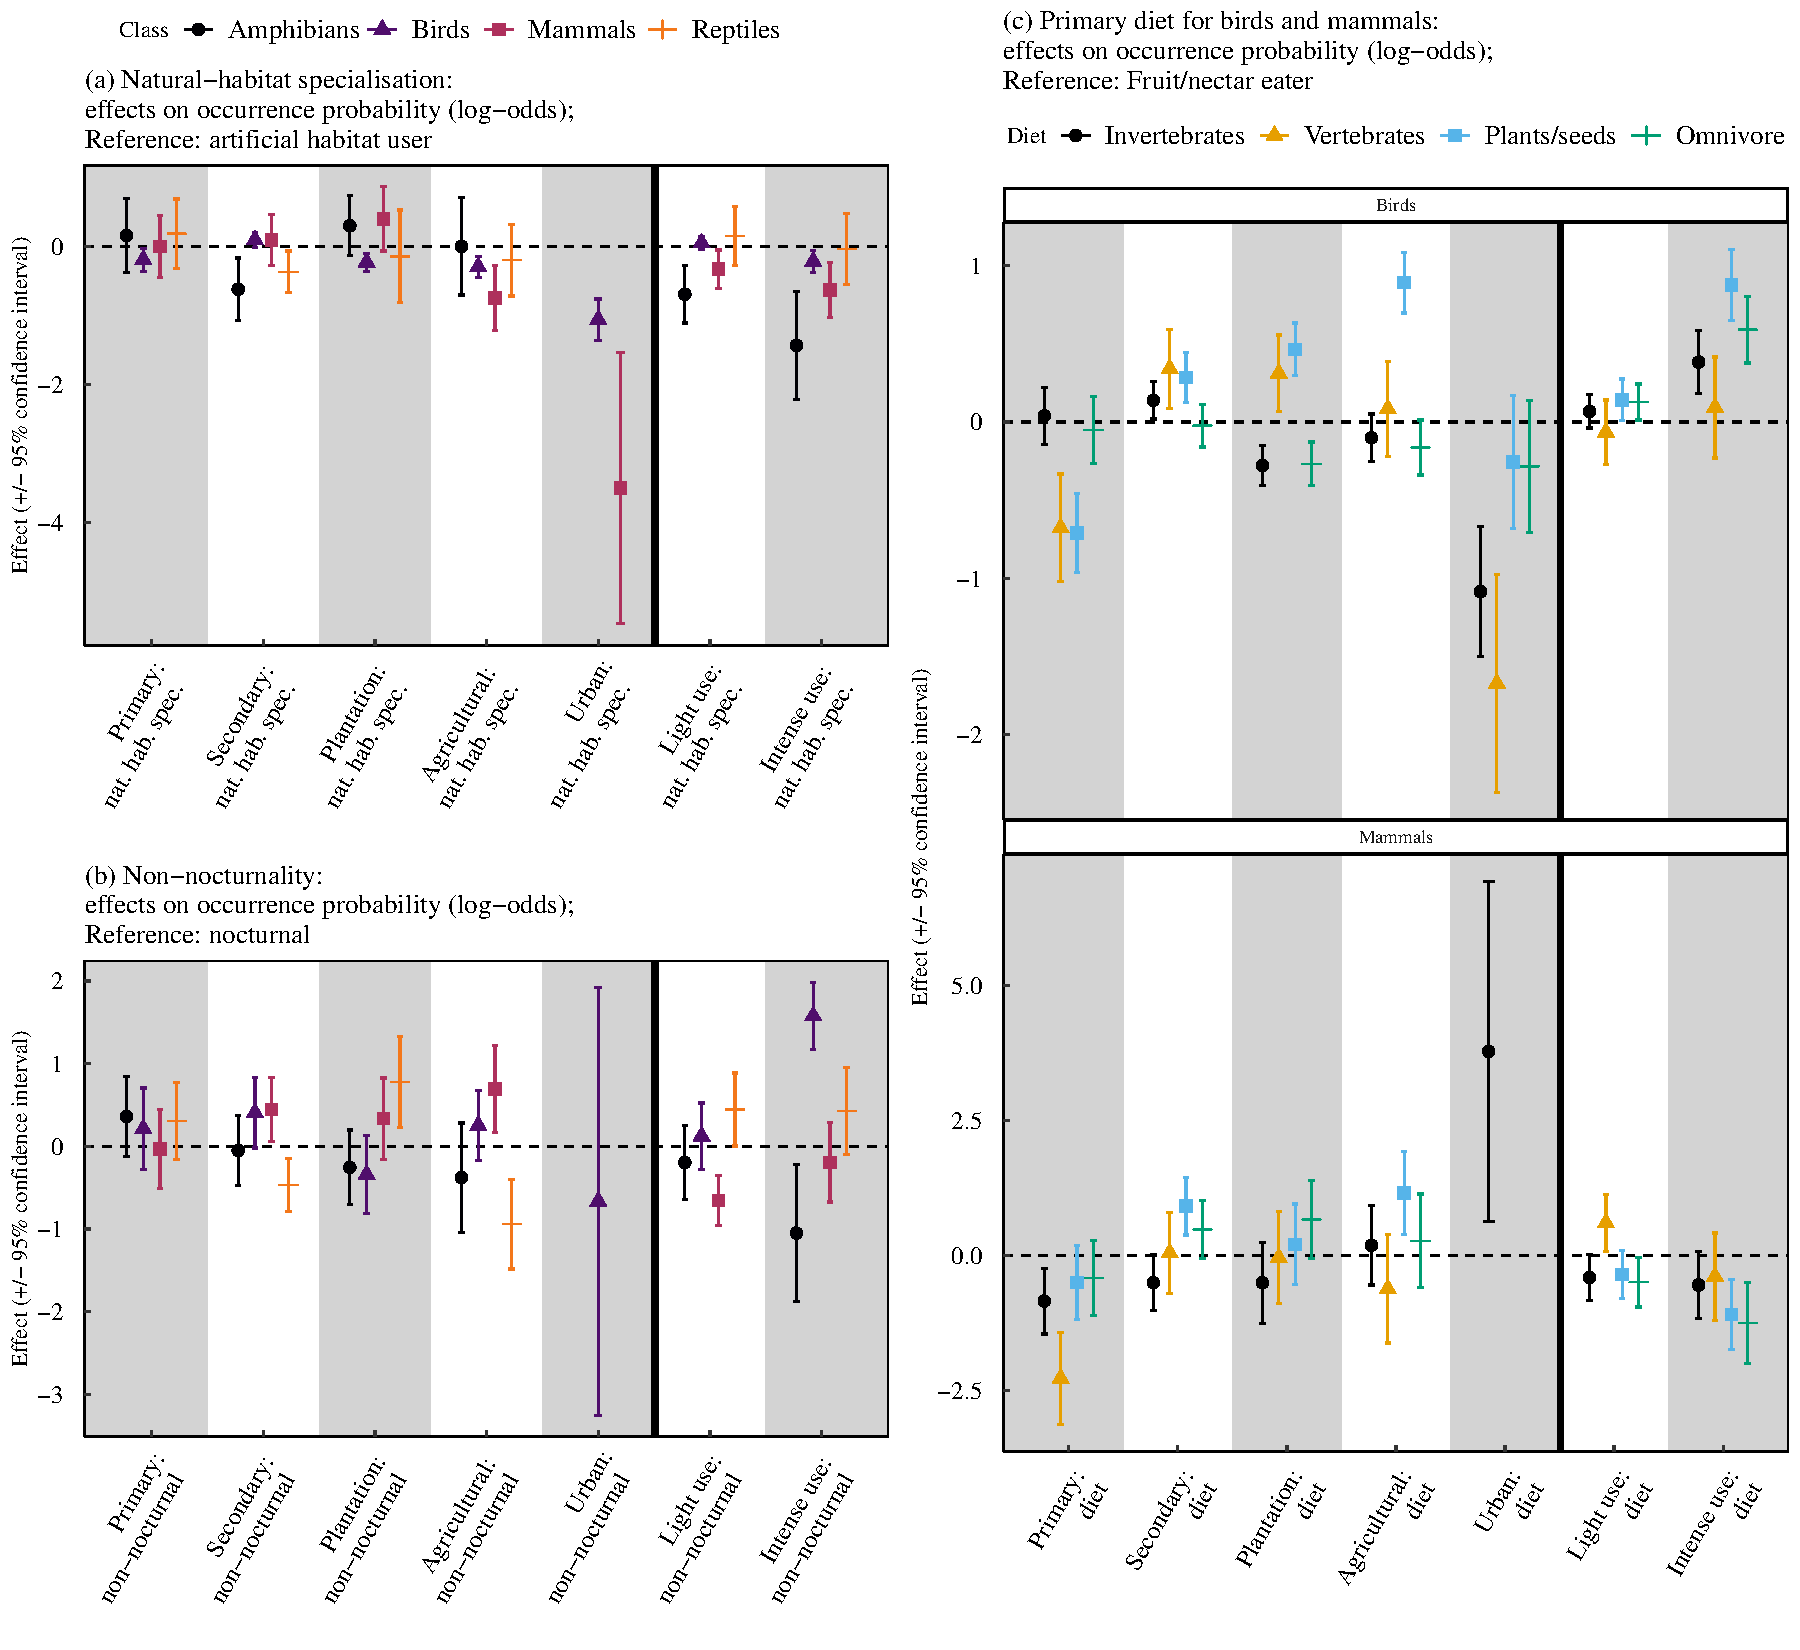
\includegraphics[scale=0.6]{Supporting/Chapter4/Figures/Full_LU_models_effects/Land_use_categorical_traits}
\caption[Effects of categorical traits on species probability of occurrence in the different land-use types, estimated from the full (all-predictor) models fitted in each class]{\textbf{Effects of categorical traits on species probability of occurrence in the different land-use types, estimated from the full (all-predictor) models fitted in each class.} The estimated effects correspond to those of the interaction terms between land use and each trait (as well as the interaction terms between land-use intensity and each trait). Hence, for each trait, the `0' baseline represents the reference level of the trait, and the effects show how any other trait level affects occurrence probability. For diet, I only show effects for mammals and birds because the full models did not include diet for reptiles and amphibians. Effects for urban reptiles could not be estimated are weren't any sampled sites. Primary: primary vegetation; Secondary: secondary vegetation; plantation: plantation forest; agricultural: cropland and pasture.}
\label{SI_4_Figure8}
\end{figure}

%% estimated slopes
\begin{figure}[h!]
\centering
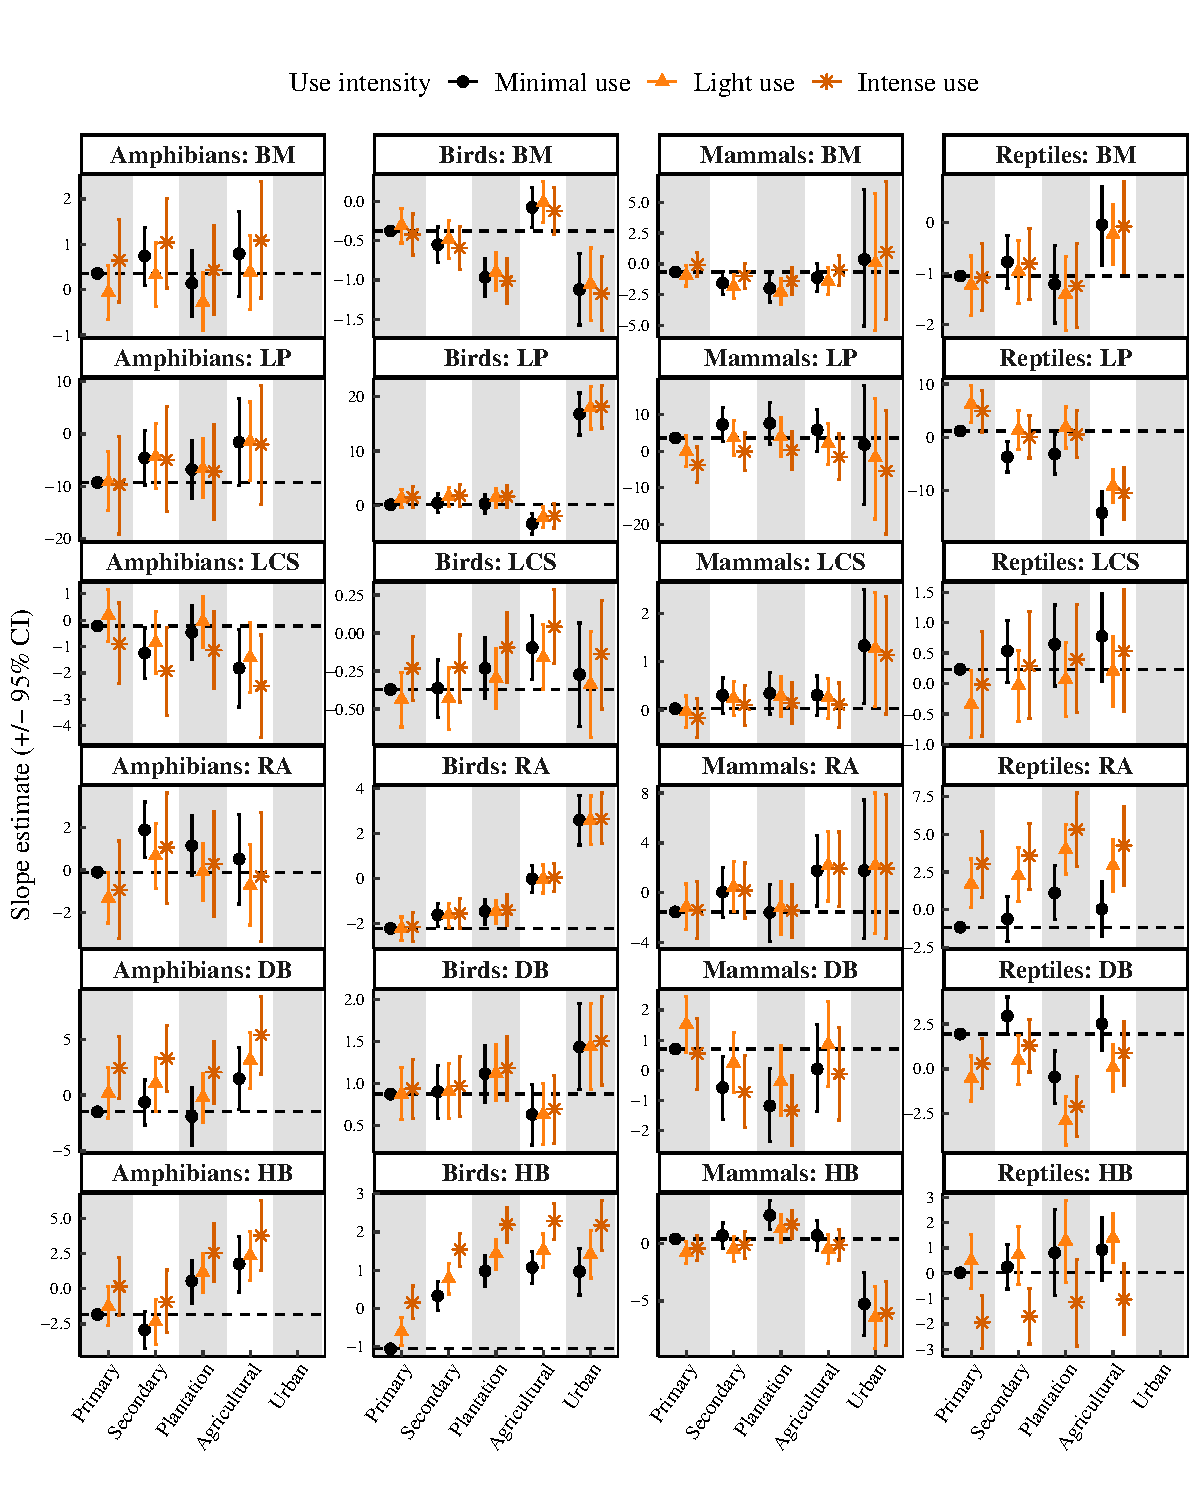
\includegraphics[scale=0.8]{Supporting/Chapter4/Figures/Full_LU_models_effects/Slopes_LU}
\caption[Effects of land use and land-use intensity on the slope of the relationships between occurrence probability and continuous explanatory variables, for each class and each continuous variable]{\textbf{Effects of land use and land-use intensity on the slope of the relationships between occurrence probability and continuous explanatory variables, for each class and each continuous variable.} The slopes were estimated from the full (all-predictor) models fitted in each class. Each column corresponds to a class and each row corresponds to a predictor (BM=body mass; LP=lifespan proxy; LCS=litter/clutch size; RA=geographical range area; DB=diet breadth; HB=habitat breadth). I did not plot the effects for amphibians in urban land uses, and those for mammals in urban land uses (for diet breadth), because error bars were large (and all effects were null). Effects for urban reptiles could not be estimated because there  weren't any sampled sites. Primary: primary vegetation; Secondary: secondary vegetation; plantation: plantation forest; agricultural: cropland and pasture.}
\label{SI_4_Figure9}
\end{figure}

\end{comment}

\clearpage
\section{Land-use responses: occurrence probability predictions from the partial models for artificial habitat use and diel activity}

%% occurrence patterns -- specialisation
\begin{figure}[h!]
\centering
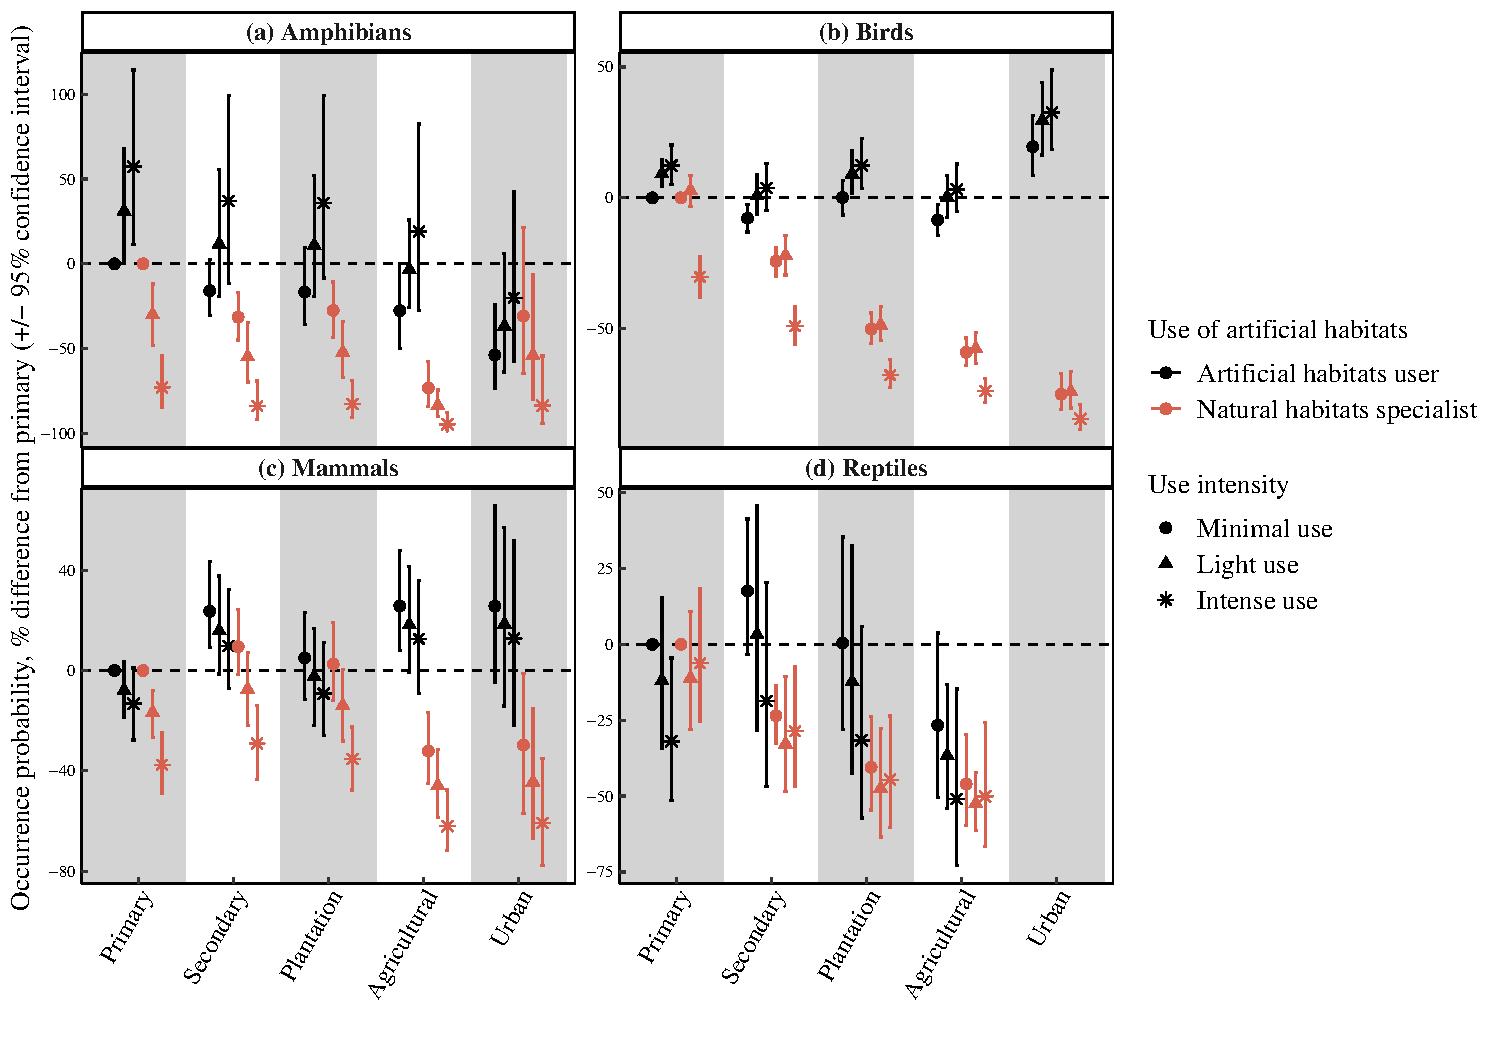
\includegraphics[scale=0.7]{Supporting/Chapter4/Figures/Partial_models_predictions/Specialisation}
\caption[Predicted occurrence probability as a function of land use, land-use intensity, artificial habitat use and their interactions in each class]{\textbf{Predicted occurrence probability as a function of land use, land-use intensity, artificial habitat use and their interactions, for each class of terrestrial vertebrates} (mean $\pm$95\% confidence interval; the predictions are rescaled with reference to minimally-used primary vegetation). The predictions were obtained from the partial models fitted in each class for artificial habitat use. Effects could not be estimated for urban reptiles, as there weren't any sampled sites. Primary: primary vegetation; Secondary: secondary vegetation; plantation: plantation forest; agricultural: cropland and pasture.}
\label{SI_4_Figure10}
\end{figure}

%% occurrence patterns -- diel activity
\begin{figure}[h!]
\centering
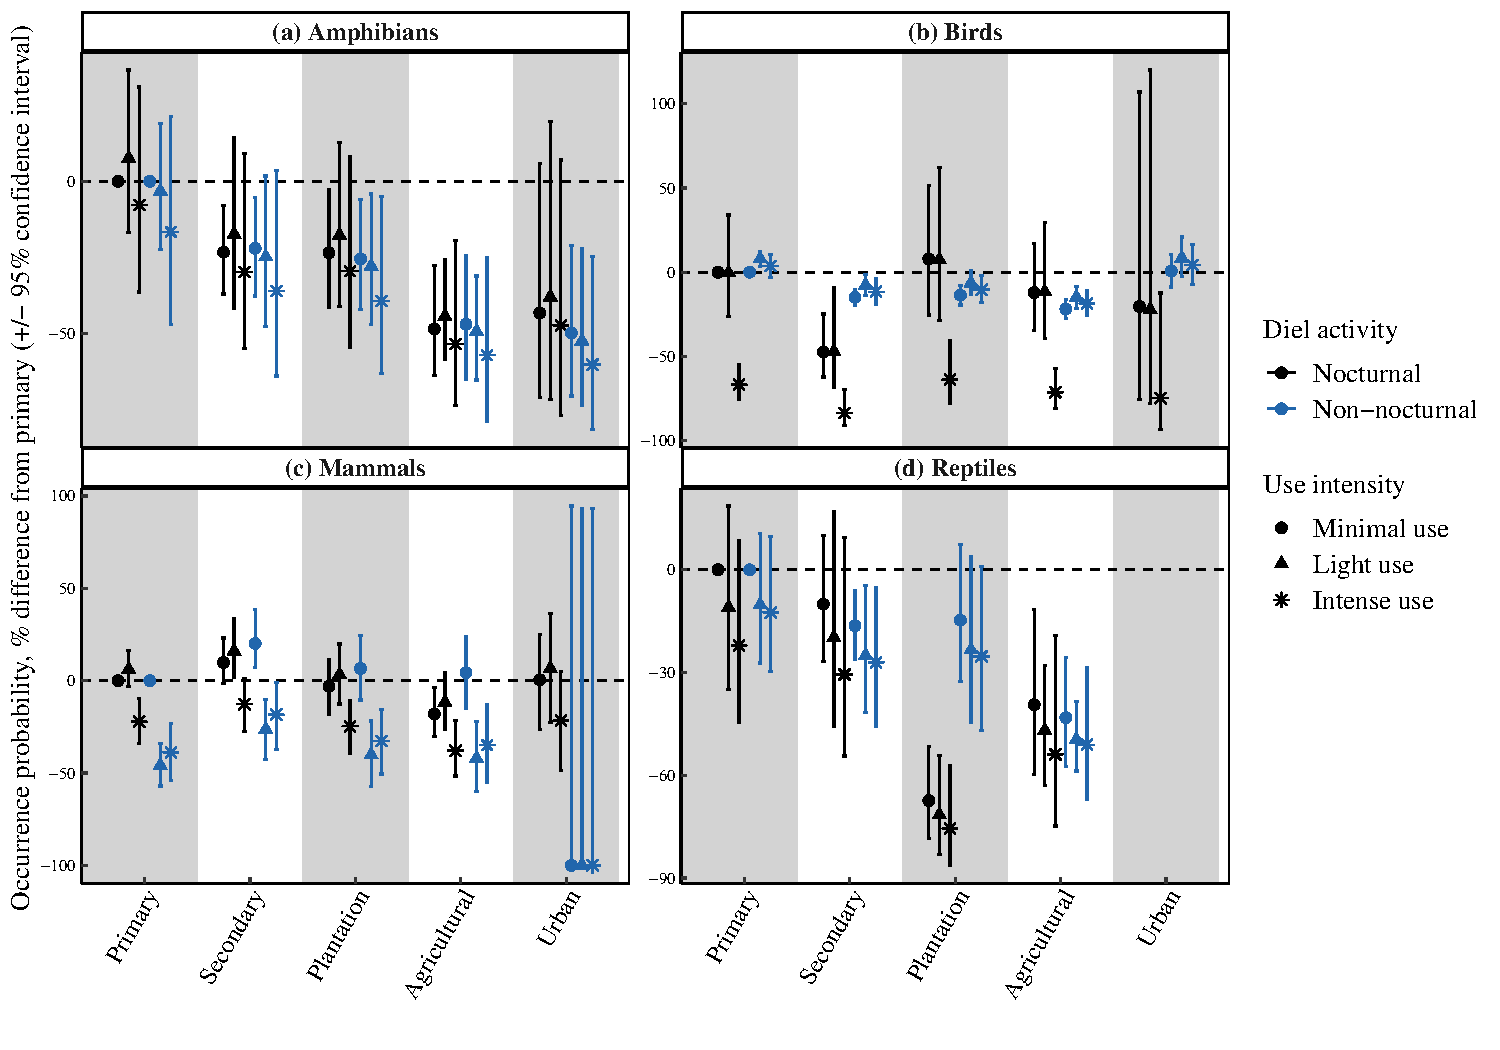
\includegraphics[scale=0.7]{Supporting/Chapter4/Figures/Partial_models_predictions/Diel_activity}
\caption[Predicted occurrence probability as a function of land use, land-use intensity, diel activity and their interactions in each class]{\textbf{Predicted occurrence probability as a function of land use, land-use intensity, diel activity and their interactions, for each class of terrestrial vertebrates} (mean $\pm$95\% confidence interval; the predictions are rescaled with reference to minimally-used primary vegetation). The predictions were obtained from the partial models fitted in each class for diel activity. Effects could not be estimated for urban reptiles, as there weren't any sampled sites. Error bars are large for non-nocturnal urban mammals because there were very few sampled species (only five).  Primary: primary vegetation; Secondary: secondary vegetation; plantation: plantation forest; agricultural: cropland and pasture.}
\label{SI_4_Figure11}
\end{figure}


\clearpage
\section{Land-use responses: diagnostic plots for the full models} 

%% diagnostic plots (DHARMa)
\begin{figure}[h!]
\centering
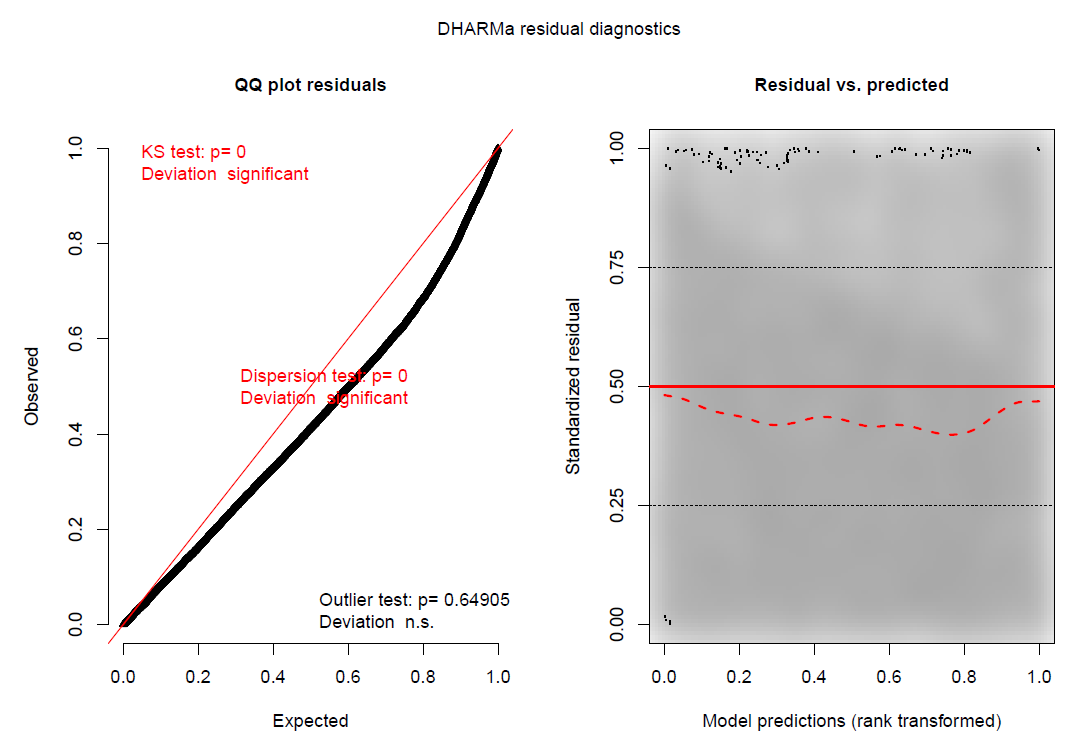
\includegraphics[scale=0.45]{Supporting/Chapter4/Figures/LU_Diag_amphibians.png}
\caption[Land-use responses: diagnostic plots for the mixed-effects model fitted on amphibians]{\textbf{Diagnostic plots for the mixed-effects model fitted on amphibians}, looking at the effects of land use, land-use intensity and the species-level ecological characteristics on species occurrence probability (full model). The diagnostic plots were obtained from the `DHARMa' R package \citep{DHARMa}.}
\label{SI_4_Figure12}
\end{figure}

\begin{figure}[h!]
\centering
\includegraphics[scale=0.45]{Supporting/Chapter4/Figures/LU_Diag_birds.png}
\caption[Land-use responses: diagnostic plots for the mixed-effects model fitted on birds]{\textbf{Diagnostic plots for the mixed-effects model fitted on birds}, looking at the effects of land use, land-use intensity and the species-level ecological characteristics on species occurrence probability (full model). The diagnostic plots were obtained from the `DHARMa' R package \citep{DHARMa}.}
\label{SI_4_Figure13}
\end{figure}

\begin{figure}[h!]
\centering
\includegraphics[scale=0.5]{Supporting/Chapter4/Figures/LU_Diag_mammals.png}
\caption[Land-use responses: diagnostic plots for the mixed-effects model fitted on mammals]{\textbf{Diagnostic plots for the mixed-effects model fitted on mammals}, looking at the effects of land use, land-use intensity and the species-level ecological characteristics on species occurrence probability (full model). The diagnostic plots were obtained from the `DHARMa' R package \citep{DHARMa}.}
\label{SI_4_Figure14}
\end{figure}

\begin{figure}[h!]
\centering
\includegraphics[scale=0.5]{Supporting/Chapter4/Figures/LU_Diag_reptiles.png}
\caption[Land-use responses: diagnostic plots for the mixed-effects model fitted on reptiles]{\textbf{Diagnostic plots for the mixed-effects model fitted on reptiles}, looking at the effects of land use, land-use intensity and the species-level ecological characteristics on species occurrence probability (full model). The diagnostic plots were obtained from the `DHARMa' R package \citep{DHARMa}.}
\label{SI_4_Figure15}
\end{figure}

\clearpage

\begin{comment}
\section{Land-use responses: estimated effects from a Bayesian framework (MCMCglmm, \citep{MCMCglmm})} 
%% Models estimates from Bayesian approach - 
%% effects of categorical traits


\begin{figure}[h!]
\centering
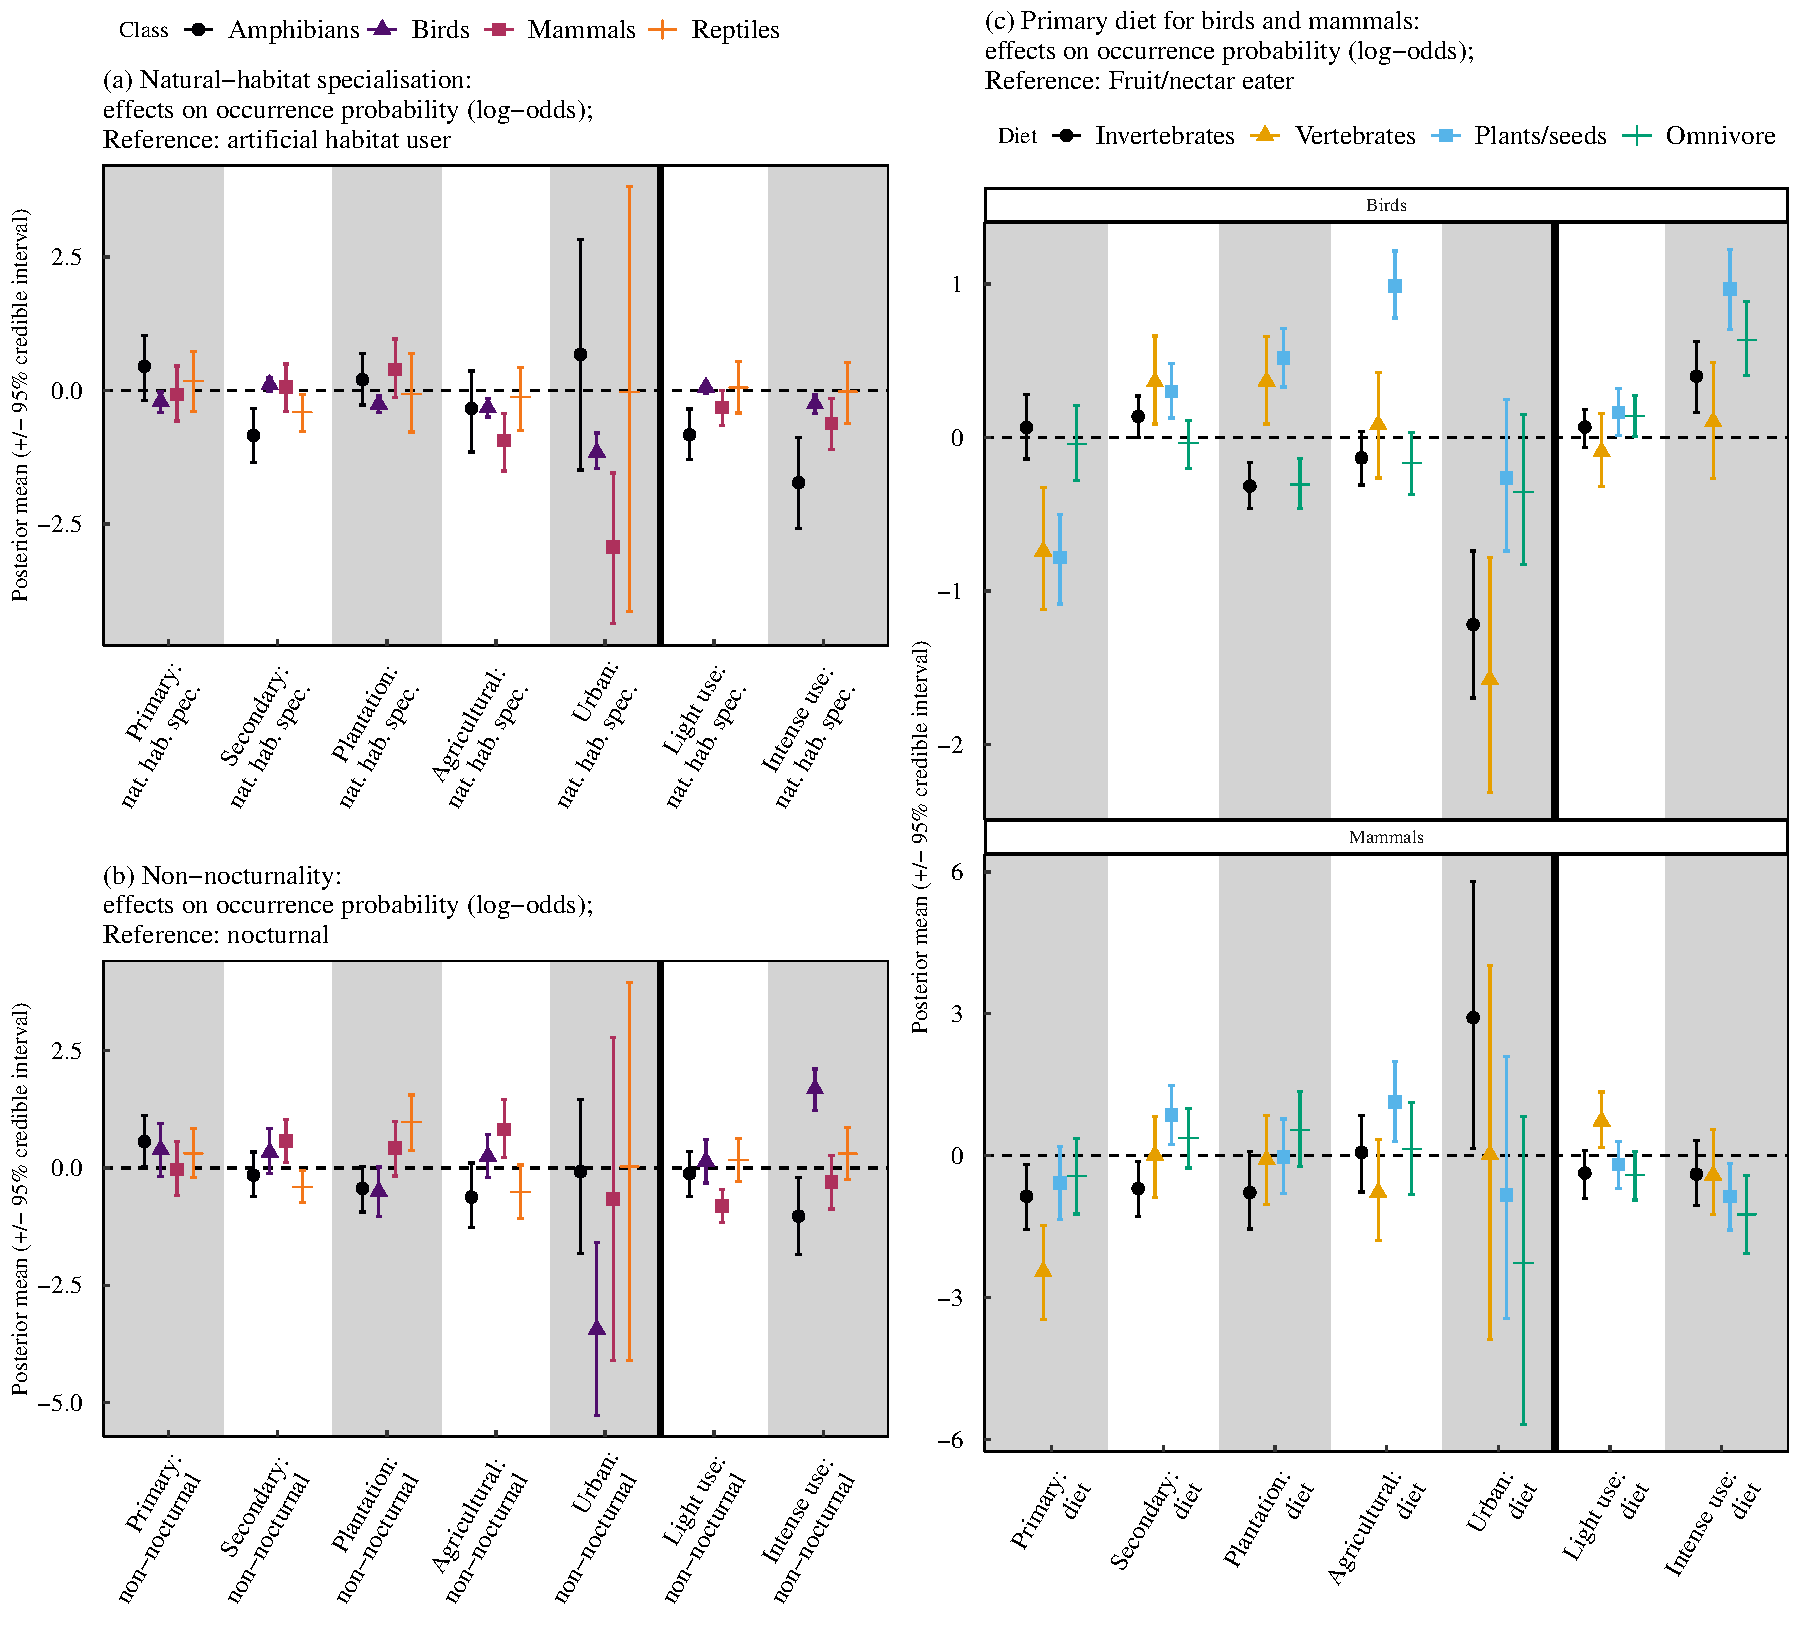
\includegraphics[scale=0.6]{Supporting/Chapter4/Figures/MCMCglmm_Land_use_categorical_traits}
\caption[Effects of categorical traits on species probability of occurrence in the different land-use types, estimated from the full (all-predictor) models fitted in each class with a Bayesian approach]{\textbf{Effects of categorical traits on species probability of occurrence in the different land-use types, estimated from the full (all-predictor) models fitted in each class with a Bayesian approach, using the `MCMCglmm' R package \citep{MCMCglmm}.} The estimated effects correspond to those of the interaction terms between land use and each trait (as well as the interaction terms between land-use intensity and each trait). Hence, for each trait, the `0' baseline represents the reference level of the trait, and the effects show how any other trait level affects occurrence probability. For diet, I only show effects for mammals and birds because the full models did not include diet for reptiles and amphibians. Effects for urban reptiles could not be estimated are weren't any sampled sites. Primary: primary vegetation; Secondary: secondary vegetation; plantation: plantation forest; agricultural: cropland and pasture.}
\label{SI_4_Figure16}
\end{figure}

%% effects of continuous traits


\begin{figure}[h!]
\centering
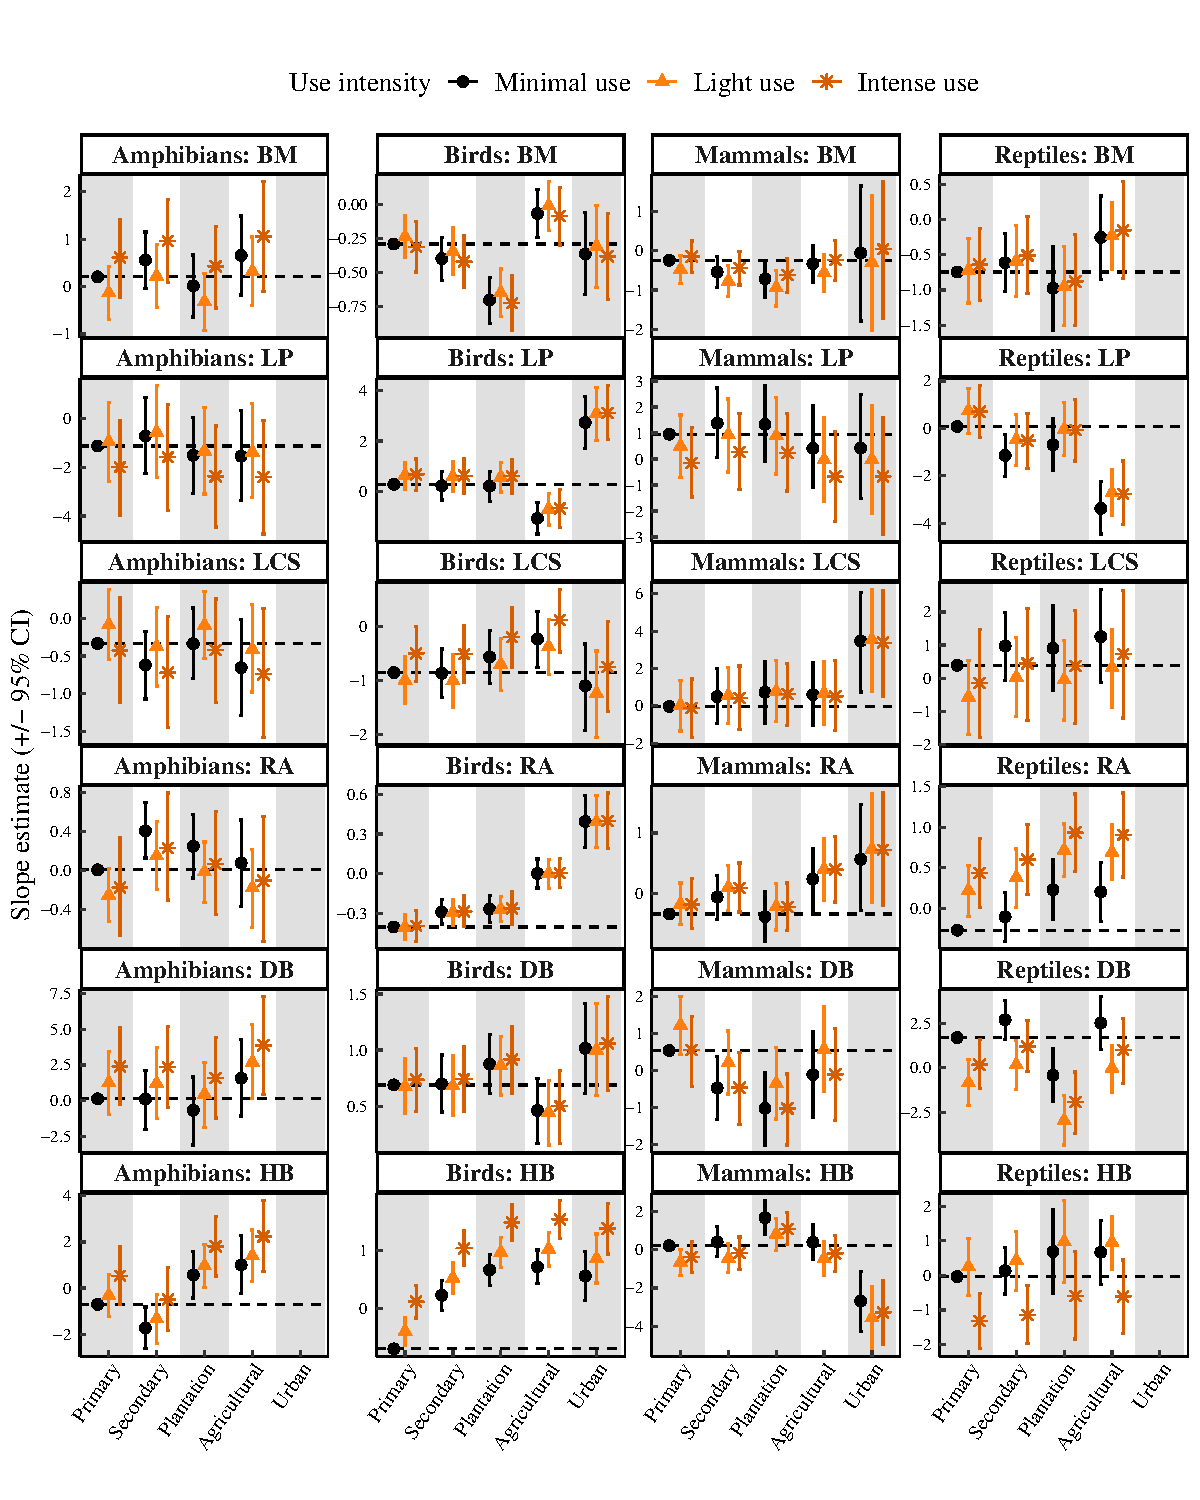
\includegraphics[scale=0.75]{Supporting/Chapter4/Figures/Slopes_LU_mcmcglmm}
\caption[Effects of land use and land-use intensity on the slope of the relationships between occurrence probability and continuous explanatory variables, for each class and each predictor, from the models fitted using a Bayesian approach]{\textbf{Effects of land use and land-use intensity on the slope of the relationships between occurrence probability and continuous explanatory variables, for each class and each predictor.} The slopes were estimated from the full (all-predictor) models fitted in each class with a Bayesian approach, using the `MCMCglmm' R \citep{MCMCglmm}. Each column corresponds to a class and each row corresponds to a predictor (BM=body mass; LP=lifespan proxy; LCS=litter/clutch size; RA=geographical range area; DB=diet breadth; HB=habitat breadth). I did not plot the effects for amphibians in urban land uses, and those for mammals in urban land uses (for diet breadth), because error bars were large (and all effects were null). Effects for urban reptiles could not be estimated are weren't any sampled sites. Primary: primary vegetation; Secondary: secondary vegetation; plantation: plantation forest; agricultural: cropland and pasture.}
\label{SI_4_Figure17}
\end{figure}

\clearpage

\end{comment}

\section{Climate-change sensitivity: model summaries and diagnostic plots}

\subsection{Summaries \& diagnostic plots for models fitted on species with range area $>$100 km\textbf{$^2$})}

%%%%%%%% Amphibians
\begin{table}[!h]
\renewcommand{\baselinestretch}{1}
\renewcommand{\arraystretch}{1}
\begin{center}\fontsize{9}{11}\selectfont
  \caption[Summary for the PGLS model fitted on amphibians]{\textbf{Summary for the PGLS model fitted on amphibians, investigating associations between species-level ecological characteristics and climate-change sensitivity,} excluding species whose range area was $\leqslant$100 km\textbf{$^2$} (sample size: n=4,537).} 
  \label{SI_4_Table14} 
\begin{tabular}{@{\extracolsep{5pt}} ccccc} 
\\[-1.8ex]\hline 
\hline \\[-1.8ex] 
 & Estimate & Std. Error & t value & Pr(\textgreater \textbar t\textbar ) \\ 
\hline \\[-1.8ex] 
Intercept & $1.15$ & $0.21$ & $5.49$ & $<0.001$ \\ 
log$_{10}$(Body mass) & $$-$1.97$ & $0.61$ & $$-$3.22$ & $0.001$ \\ 
log$_{10}$(Body mass)$^2$ & $$-$0.26$ & $0.42$ & $$-$0.60$ & $0.55$ \\ 
log$_{10}$(Body mass)$^3$ & $0.46$ & $0.37$ & $1.24$ & $0.22$ \\ 
log$_{10}$(Lifespan proxy) & $$-$0.21$ & $0.59$ & $$-$0.36$ & $0.72$ \\ 
log$_{10}$(Lifespan proxy)$^2$ & $$-$0.14$ & $0.43$ & $$-$0.32$ & $0.75$ \\ 
log$_{10}$(Lifespan proxy)$^3$ & $0.58$ & $0.35$ & $1.66$ & $0.10$ \\ 
log$_{10}$(Litter/clutch size) & $1.59$ & $0.54$ & $2.96$ & $0.003$ \\ 
log$_{10}$(Litter/clutch size)$^2$ & $$-$0.06$ & $0.38$ & $$-$0.16$ & $0.87$ \\ 
log$_{10}$(Litter/clutch size)$^3$ & $$-$0.74$ & $0.31$ & $$-$2.37$ & $0.02$ \\ 
log$_{10}$(Range area) & $$-$26.60$ & $0.34$ & $$-$77.15$ & $<0.001$ \\ 
log$_{10}$(Range area)$^2$ & $4.27$ & $0.29$ & $14.57$ & $<0.001$ \\ 
log$_{10}$(Range area)$^3$ & $$-$1.65$ & $0.28$ & $$-$5.96$ & $<0.001$ \\ 
square-root(Habitat breadth) & $$-$2.26$ & $0.43$ & $$-$5.32$ & $<0.001$ \\ 
square-root(Habitat breadth)$^2$  & $0.81$ & $0.30$ & $2.67$ & $0.01$ \\ 
square-root(Habitat breadth)$^3$  & $$-$0.59$ & $0.28$ & $$-$2.10$ & $0.04$ \\ 
Specialisation: Natural habitat specialist & $0.02$ & $0.01$ & $1.85$ & $0.06$ \\ 
Diel activity: Non-nocturnal & $0.04$ & $0.01$ & $3.28$ & $0.001$ \\ 
Primary diet: Omnivore & $0.01$ & $0.03$ & $0.29$ & $0.77$ \\ 
Primary diet: Plants/seeds & $0.04$ & $0.13$ & $0.31$ & $0.76$ \\ 
Primary diet: Vertebrates & $0.13$ & $0.15$ & $0.87$ & $0.39$ \\ 
\hline \\[-1.8ex] 
\end{tabular} 
\end{center}
\end{table} 

\vspace{-1.2cm}

\begin{figure}[h!]
\centering
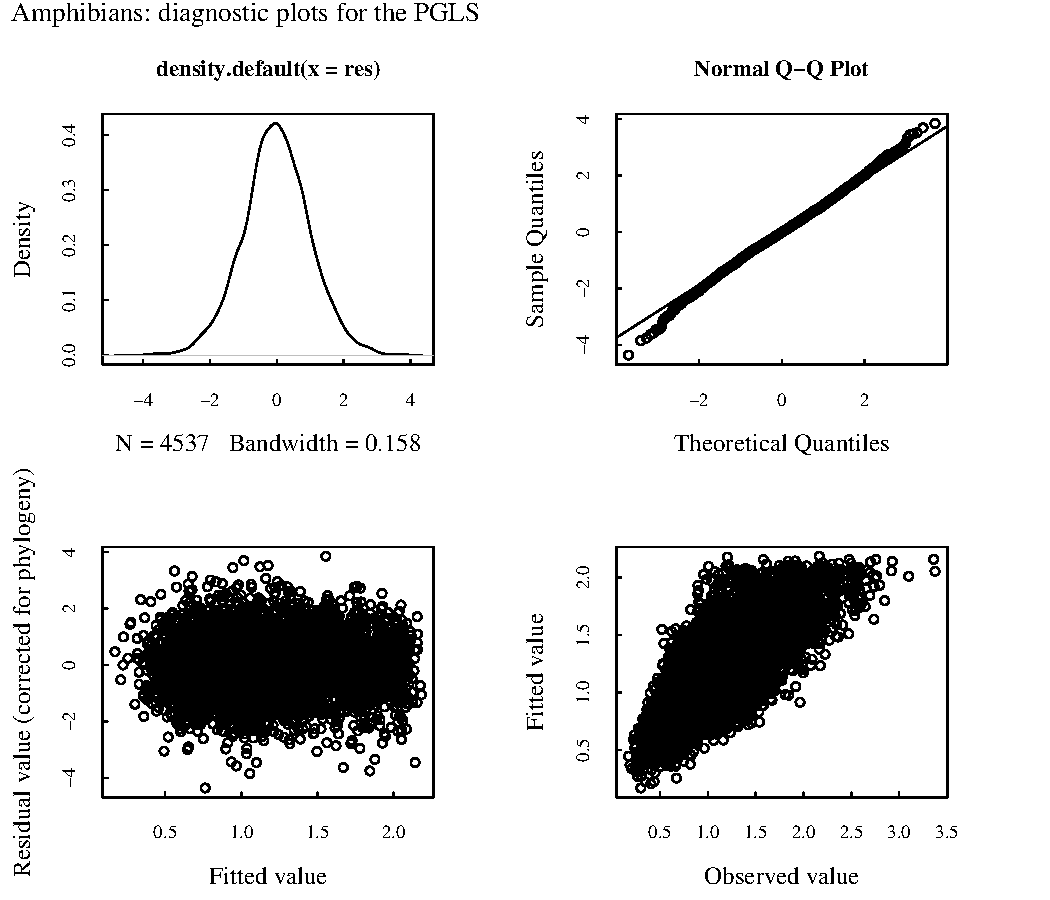
\includegraphics[scale=0.58, trim={0 0 0 20},clip]{Supporting/Chapter4/Figures/PGLS_diag_amphibians}
\caption[Diagnostic plots for the PGLS model fitted on amphibians]{\textbf{Diagnostic plots for the PGLS model fitted on amphibians, investigating associations between species-level ecological characteristics and climate-change sensitivity,} excluding species whose range area was $\leqslant$100 km\textbf{$^2$} (sample size: n=4,537).}
\label{SI_4_Figure18}
\end{figure}

\clearpage
%%%%%%%%%%%% Birds
\begin{table}[!h]
\renewcommand{\baselinestretch}{1}
\renewcommand{\arraystretch}{1}
\begin{center}\fontsize{9}{11}\selectfont
  \caption[Summary for the PGLS model fitted on birds]{\textbf{Summary for the PGLS model fitted on birds, investigating associations between species-level ecological characteristics and climate-change sensitivity,} excluding species whose range area was $\leqslant$100 km\textbf{$^2$} (sample size: n=10,198).} 
  \label{SI_4_Table15} 
\begin{tabular}{@{\extracolsep{5pt}} ccccc} 
\\[-1.8ex]\hline 
\hline \\[-1.8ex] 
 & Estimate & Std. Error & t value & Pr(\textgreater \textbar t\textbar ) \\ 
\hline \\[-1.8ex] 
Intercept & $0.64$ & $0.08$ & $7.91$ & $<0.001$ \\ 
log$_{10}$(Body mass) & $2.24$ & $0.67$ & $3.36$ & $0.001$ \\ 
log$_{10}$(Body mass)$^2$ & $0.16$ & $0.42$ & $0.37$ & $0.71$ \\ 
log$_{10}$(Body mass)$^3$ & $$-$0.22$ & $0.37$ & $$-$0.60$ & $0.55$ \\ 
log$_{10}$(Lifespan proxy) & $$-$0.23$ & $0.59$ & $$-$0.38$ & $0.70$ \\ 
log$_{10}$(Lifespan proxy)$^2$ & $$-$0.84$ & $0.39$ & $$-$2.16$ & $0.03$ \\ 
log$_{10}$(Lifespan proxy)$^3$ & $$-$0.10$ & $0.28$ & $$-$0.36$ & $0.72$ \\ 
log$_{10}$(Litter/clutch size) & $3.72$ & $0.39$ & $9.46$ & $<0.001$ \\ 
log$_{10}$(Litter/clutch size)$^2$ & $$-$0.42$ & $0.33$ & $$-$1.26$ & $0.21$ \\ 
log$_{10}$(Litter/clutch size)$^3$ & $$-$0.40$ & $0.27$ & $$-$1.47$ & $0.14$ \\ 
log$_{10}$(Range area) & $$-$30.69$ & $0.27$ & $$-$113.09$ & $<0.001$ \\ 
log$_{10}$(Range area)$^2$ & $7.22$ & $0.24$ & $29.92$ & $<0.001$ \\ 
log$_{10}$(Range area)$^3$ & $$-$2.73$ & $0.23$ & $$-$11.74$ & $<0.001$ \\ 
square-root(Habitat breadth) & $0.86$ & $0.33$ & $2.59$ & $0.01$ \\ 
square-root(Habitat breadth)$^2$ & $$-$0.89$ & $0.24$ & $$-$3.63$ & $<0.001$ \\ 
square-root(Habitat breadth)$^3$ & $$-$0.22$ & $0.23$ & $$-$0.95$ & $0.34$ \\ 
square-root(Diet breadth) & $$-$0.50$ & $0.31$ & $$-$1.64$ & $0.10$ \\ 
square-root(Diet breadth)$^2$ & $$-$0.11$ & $0.25$ & $$-$0.44$ & $0.66$ \\ 
square-root(Diet breadth)$^3$ & $0.32$ & $0.24$ & $1.36$ & $0.18$ \\ 
Specialisation: Natural habitat specialist & $0.06$ & $0.01$ & $10.13$ & $<0.001$ \\ 
Diel activity: Non-nocturnal& $$-$0.02$ & $0.04$ & $$-$0.66$ & $0.51$ \\ 
Primary diet: Invertebrates & $0.06$ & $0.01$ & $5.53$ & $<0.001$ \\ 
Primary diet: Omnivores & $0.02$ & $0.01$ & $2.09$ & $0.04$ \\ 
Primary diet: Plants/seeds & $0.06$ & $0.01$ & $4.69$ & $<0.001$ \\ 
Primary diet: Vertebrates & $0.01$ & $0.02$ & $0.83$ & $0.41$ \\ 
\hline \\[-1.8ex] 
\end{tabular} 
\end{center}
\end{table} 

\vspace{-1cm}
\begin{figure}[h!]
\centering
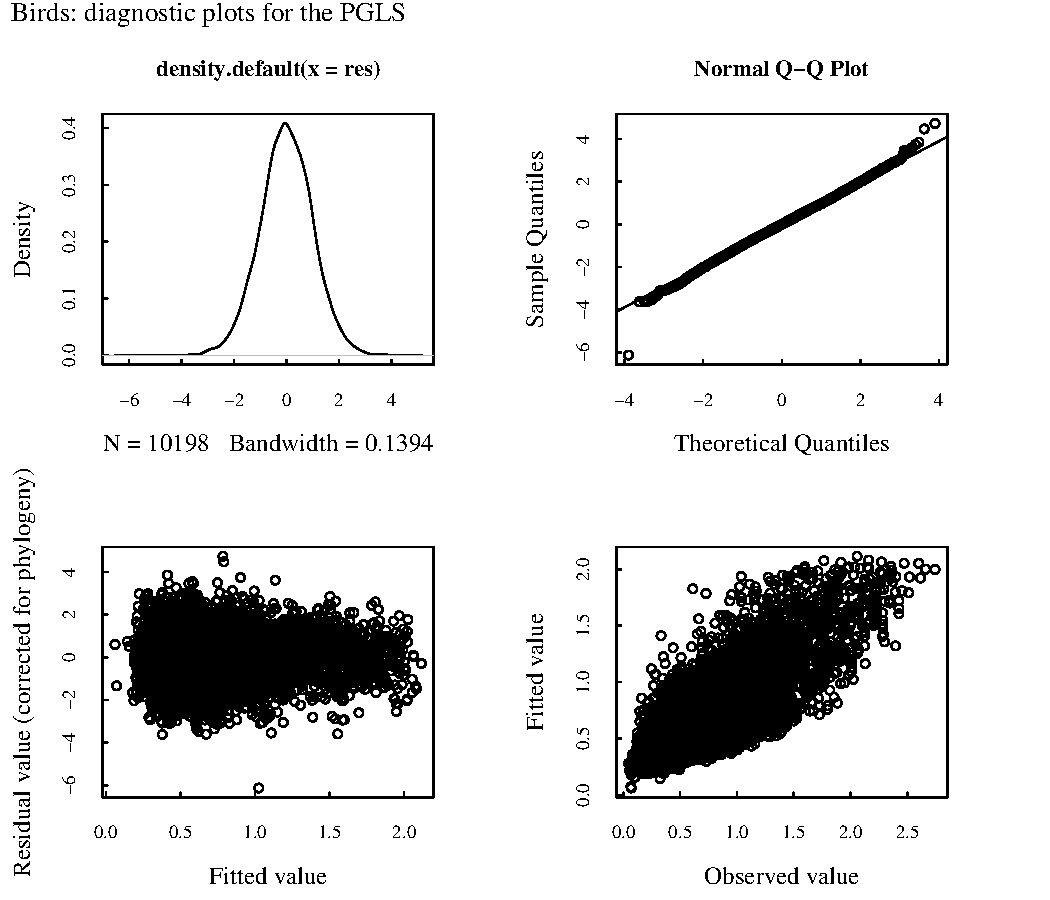
\includegraphics[scale=0.58,trim={0 0 0 20},clip]{Supporting/Chapter4/Figures/PGLS_diag_birds}
\caption[Diagnostic plots for the PGLS model fitted on birds]{\textbf{Diagnostic plots for the PGLS model fitted on birds, investigating associations between species-level ecological characteristics and climate-change sensitivity,} excluding species whose range area was $\leqslant$100 km\textbf{$^2$} (sample size: n=10,198).}
\label{SI_4_Figure19}
\end{figure}

\clearpage
%%%%%%%%%%%%%%% Mammals
\begin{table}[!h]
\renewcommand{\baselinestretch}{1}
\renewcommand{\arraystretch}{1}
\begin{center}\fontsize{9}{11}\selectfont 
  \caption[Summary for the PGLS model fitted on mammals]{\textbf{Summary for the PGLS model fitted on mammals, investigating associations between species-level ecological characteristics and climate-change sensitivity,} excluding species whose range area was $\leqslant$100 km\textbf{$^2$} (sample size: n=4,712).} 
  \label{SI_4_Table16} 
\begin{tabular}{@{\extracolsep{5pt}} ccccc} 
\\[-1.8ex]\hline 
\hline \\[-1.8ex] 
 & Estimate & Std. Error & t value & Pr(\textgreater \textbar t\textbar ) \\ 
\hline \\[-1.8ex] 
Intercept & $0.84$ & $0.16$ & $5.37$ & $<0.001$ \\ 
log$_{10}$(Body mass) & $$-$4.62$ & $0.94$ & $$-$4.93$ & $<0.001$ \\ 
log$_{10}$(Body mass)$^2$ & $0.40$ & $0.56$ & $0.72$ & $0.47$ \\ 
log$_{10}$(Body mass)$^3$ & $0.59$ & $0.44$ & $1.33$ & $0.18$ \\ 
log$_{10}$(Lifespan proxy) & $1.60$ & $1.03$ & $1.55$ & $0.12$ \\ 
log$_{10}$(Lifespan proxy)$^2$ & $$-$0.79$ & $0.49$ & $$-$1.60$ & $0.11$ \\ 
log$_{10}$(Lifespan proxy)$^3$ & $$-$0.15$ & $0.43$ & $$-$0.35$ & $0.73$ \\ 
log$_{10}$(Litter/clutch size) & $3.29$ & $0.71$ & $4.63$ & $<0.001$ \\ 
log$_{10}$(Litter/clutch size)$^2$ & $0.06$ & $0.42$ & $0.14$ & $0.89$ \\ 
log$_{10}$(Litter/clutch size)$^3$ & $$-$0.16$ & $0.33$ & $$-$0.47$ & $0.64$ \\ 
log$_{10}$(Range area) & $$-$24.17$ & $0.31$ & $$-$78.21$ & $<0.001$ \\ 
log$_{10}$(Range area)$^2$ & $4.15$ & $0.28$ & $15.09$ & $<0.001$ \\ 
log$_{10}$(Range area)$^3$ & $$-$0.90$ & $0.26$ & $$-$3.45$ & $0.001$ \\ 
square-root(Habitat breadth) & $$-$1.24$ & $0.34$ & $$-$3.60$ & $<0.001$ \\ 
square-root(Habitat breadth)$^2$ & $0.22$ & $0.27$ & $0.82$ & $0.41$ \\ 
square-root(Habitat breadth)$^3$ & $$-$0.03$ & $0.26$ & $$-$0.10$ & $0.92$ \\ 
square-root(Diet breadth) & $$-$1.21$ & $0.47$ & $$-$2.55$ & $0.01$ \\ 
square-root(Diet breadth)$^2$ & $0.33$ & $0.36$ & $0.91$ & $0.36$ \\ 
square-root(Diet breadth)$^3$ & $0.11$ & $0.34$ & $0.33$ & $0.74$ \\ 
Specialisation: Natural habitat specialist & $0.04$ & $0.01$ & $3.22$ & $0.001$ \\ 
Diel activity: Non-nocturnal & $0.003$ & $0.01$ & $0.23$ & $0.82$ \\ 
Primary diet: Invertebrates & $$-$0.02$ & $0.03$ & $$-$0.62$ & $0.54$ \\ 
Primary diet: Omnivores & $$-$0.02$ & $0.03$ & $$-$0.77$ & $0.44$ \\ 
Primary diet: Plants/seeds & $0.03$ & $0.02$ & $1.32$ & $0.19$ \\ 
Primary diet: Vertebrates & $$-$0.04$ & $0.04$ & $$-$0.98$ & $0.33$ \\ 
\hline \\[-1.8ex] 
\end{tabular} 
\end{center}
\end{table} 

\begin{figure}[h!]
\centering
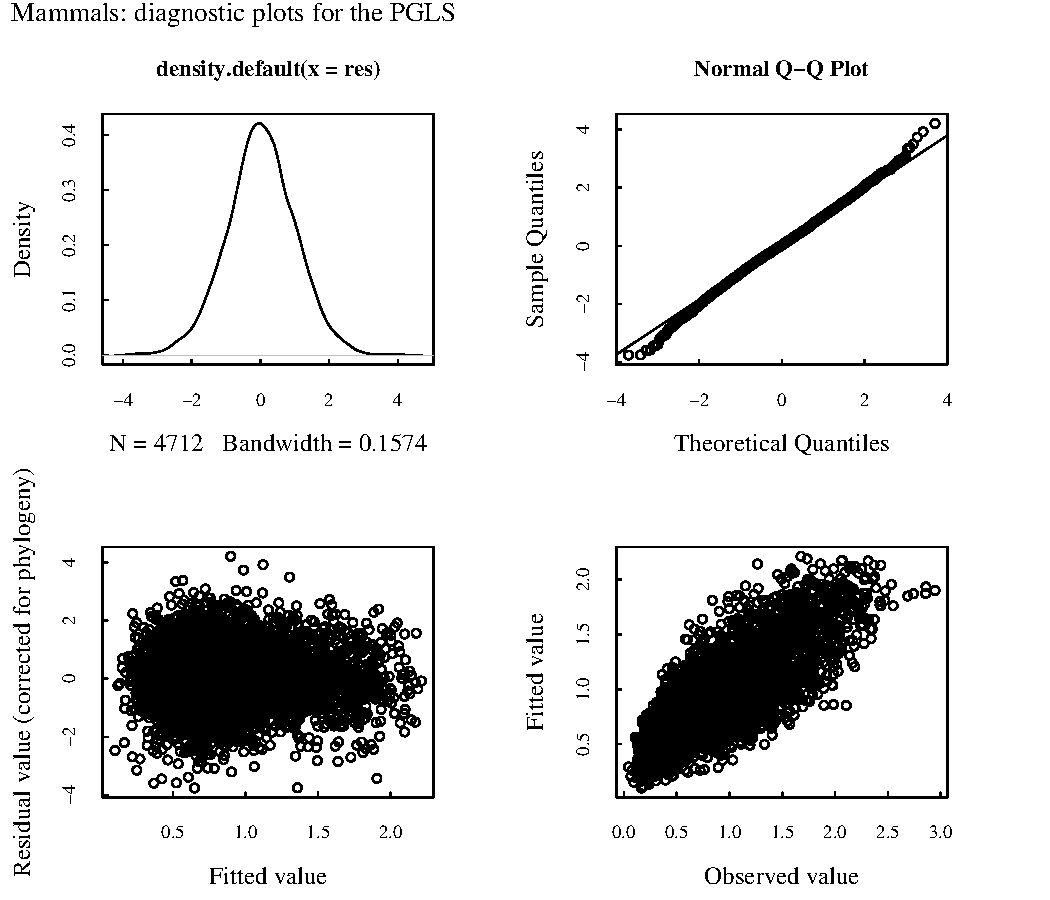
\includegraphics[scale=0.58,trim={0 0 0 20},clip]{Supporting/Chapter4/Figures/PGLS_diag_mammals}
\caption[Diagnostic plots for the PGLS model fitted on mammals]{\textbf{Diagnostic plots for the PGLS model fitted on mammals, investigating associations between species-level ecological characteristics and climate-change sensitivity,} excluding species whose range area was $\leqslant$100 km\textbf{$^2$} (sample size: n=4,712).}
\label{SI_4_Figure20}
\end{figure}

%%%%%%%%%%%%%%% Reptiles

\begin{table}[!h] 
\renewcommand{\baselinestretch}{1}
\renewcommand{\arraystretch}{1}
\begin{center}\fontsize{9}{11}\selectfont 
  \caption[Summary for the PGLS model fitted on reptiles]{\textbf{Summary for the PGLS model fitted on reptiles, looking at the effects of species-level ecological characteristics on climate-change sensitivity,} excluding species whose range area was $\leqslant$100 km\textbf{$^2$} (sample size: n=7,330).} 
  \label{SI_4_Table17} 
\begin{tabular}{@{\extracolsep{5pt}} ccccc} 
\\[-1.8ex]\hline 
\hline \\[-1.8ex] 
 & Estimate & Std. Error & t value & Pr(\textgreater \textbar t\textbar ) \\ 
\hline \\[-1.8ex] 
Intercept & $1.02$ & $0.13$ & $7.70$ & $<0.001$ \\ 
log$_{10}$(Body mass) & $$-$4.62$ & $0.62$ & $$-$7.47$ & $<0.001$ \\ 
log$_{10}$(Body mass)$^2$ & $0.97$ & $0.41$ & $2.35$ & $0.02$ \\ 
log$_{10}$(Body mass)$^3$ & $$-$0.96$ & $0.33$ & $$-$2.90$ & $0.004$ \\ 
log$_{10}$(Lifespan proxy) & $0.89$ & $0.51$ & $1.74$ & $0.08$ \\ 
log$_{10}$(Lifespan proxy)$^2$ & $$-$1.27$ & $0.39$ & $$-$3.27$ & $0.001$ \\ 
log$_{10}$(Lifespan proxy)$^3$ & $$-$0.29$ & $0.33$ & $$-$0.88$ & $0.38$ \\ 
log$_{10}$(Litter/clutch size) & $0.84$ & $0.68$ & $1.24$ & $0.22$ \\ 
log$_{10}$(Litter/clutch size)$^2$ & $$-$0.34$ & $0.45$ & $$-$0.76$ & $0.45$ \\ 
log$_{10}$(Litter/clutch size)$^3$ & $0.26$ & $0.35$ & $0.74$ & $0.46$ \\ 
log$_{10}$(Range area) & $$-$31.88$ & $0.31$ & $$-$101.48$ & $<0.001$ \\ 
log$_{10}$(Range area)$^2$ & $5.15$ & $0.27$ & $19.03$ & $<0.001$\\ 
log$_{10}$(Range area)$^3$ & $$-$1.97$ & $0.26$ & $$-$7.53$ & $<0.001$ \\ 
square-root(Habitat breadth) & $0.56$ & $0.35$ & $1.59$ & $0.11$ \\ 
square-root(Habitat breadth)$^2$ & $$-$0.67$ & $0.27$ & $$-$2.49$ & $0.01$ \\ 
square-root(Habitat breadth)$^3$ & $0.05$ & $0.26$ & $0.21$ & $0.83$ \\ 
square-root(Diet breadth) & $$-$0.33$ & $0.37$ & $$-$0.90$ & $0.37$ \\ 
square-root(Diet breadth)$^2$ & $$-$0.02$ & $0.27$ & $$-$0.08$ & $0.94$ \\ 
square-root(Diet breadth)$^2$ & $0.31$ & $0.26$ & $1.22$ & $0.22$ \\ 
Specialisation: Natural habitat specialist & $0.10$ & $0.01$ & $8.50$ & $<0.001$ \\ 
Diel activity: Non-nocturnal & $$-$0.02$ & $0.01$ & $$-$1.88$ & $0.06$ \\ 
Primary diet: Omnivore & $$-$0.03$ & $0.03$ & $$-$0.92$ & $0.36$ \\ 
Primary diet: Vertebrates & $$-$0.02$ & $0.02$ & $$-$1.05$ & $0.30$ \\ 
\hline \\[-1.8ex] 
\end{tabular} 
\end{center}
\end{table} 


\begin{figure}[h!]
\centering
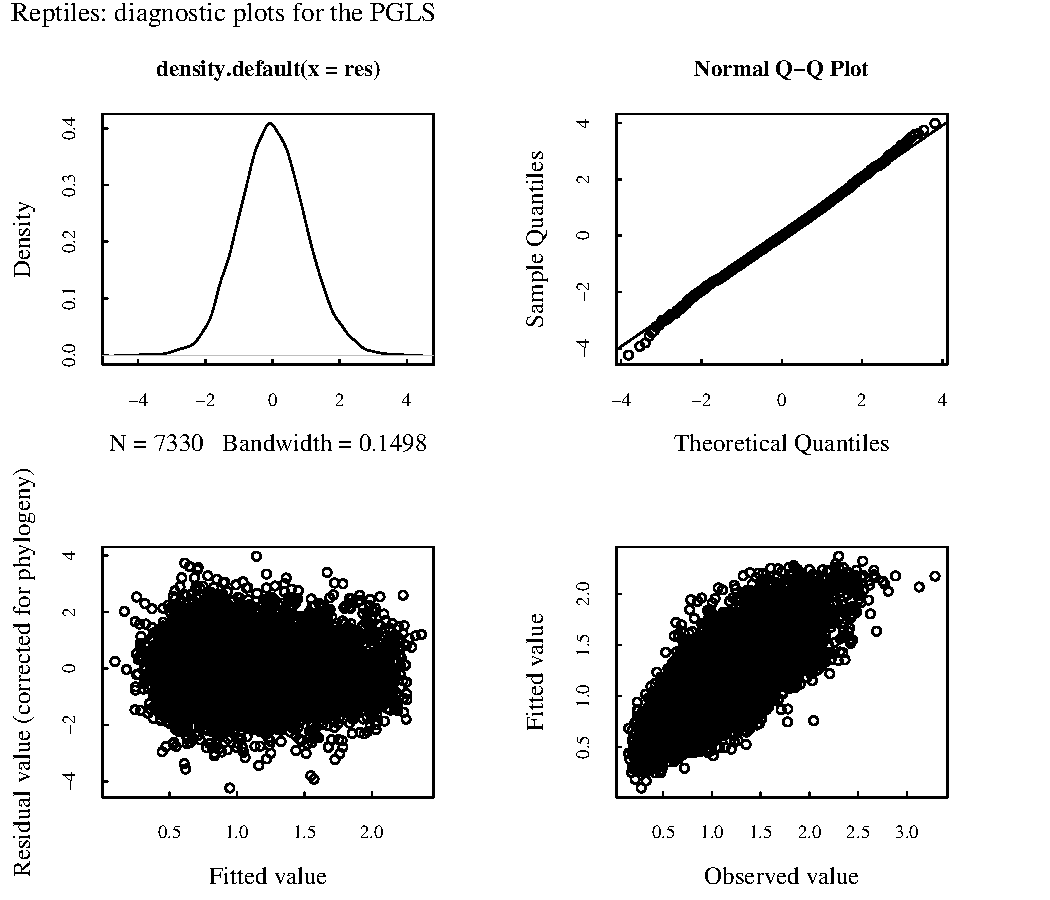
\includegraphics[scale=0.58, trim={0 0 0 20},clip]{Supporting/Chapter4/Figures/PGLS_diag_reptiles}
\caption[Diagnostic plots for the PGLS model fitted on reptiles]{\textbf{Diagnostic plots for the PGLS model fitted on reptiles, investigating associations between species-level ecological characteristics and climate-change sensitivity,} excluding species whose range area was $\leqslant$100 km\textbf{$^2$} (sample size: n=7,330).}
\label{SI_4_Figure21}
\end{figure}


\clearpage

\begin{comment}
\subsection{Summaries for the PGLS models fitted on all species (including those with range area $\leqslant$100 km\textbf{$^2$})}

\begin{table}[!h]
\renewcommand{\baselinestretch}{1}
\renewcommand{\arraystretch}{1}
\begin{center}\fontsize{9}{11}\selectfont 
  \caption[Summary for the PGLS model fitted on amphibians, with all species (including species whose range area was $\leqslant$100 km\textbf{$^2$})]{\textbf{Summary for the PGLS model fitted on amphibians, investigating associations between species-level ecological characteristics and climate-change sensitivity,} including species whose range area was $\leqslant$100 km\textbf{$^2$} (sample size: n=5,197).} 
  \label{SI_4_Table18} 
\begin{tabular}{@{\extracolsep{5pt}} ccccc} 
\\[-1.8ex]\hline 
\hline \\[-1.8ex] 
 & Estimate & Std. Error & t value & Pr(\textgreater \textbar t\textbar ) \\ 
\hline \\[-1.8ex] 
Intercept & $1.23$ & $0.20$ & $6.01$ & $<0.001$ \\ 
log$_{10}$(Body mass) & $$-$1.70$ & $0.74$ & $$-$2.29$ & $0.02$ \\ 
log$_{10}$(Body mass)$^2$ & $$-$0.56$ & $0.52$ & $$-$1.09$ & $0.28$ \\ 
log$_{10}$(Body mass)$^3$ & $0.12$ & $0.44$ & $0.27$ & $0.78$ \\ 
log$_{10}$(Lifespan proxy) & $0.46$ & $0.72$ & $0.64$ & $0.52$ \\ 
log$_{10}$(Lifespan proxy)$^2$ & $0.21$ & $0.53$ & $0.40$ & $0.69$ \\ 
log$_{10}$(Lifespan proxy)$^3$ & $0.50$ & $0.43$ & $1.17$ & $0.24$ \\ 
log$_{10}$(Litter/clutch size) & $0.95$ & $0.64$ & $1.48$ & $0.14$ \\ 
log$_{10}$(Litter/clutch size)$^2$ & $$-$0.34$ & $0.45$ & $$-$0.74$ & $0.46$ \\ 
log$_{10}$(Litter/clutch size)$^3$ & $$-$1.07$ & $0.38$ & $$-$2.79$ & $0.01$ \\ 
log$_{10}$(Range area) & $$-$28.60$ & $0.42$ & $$-$67.90$ & $<0.001$ \\ 
log$_{10}$(Range area)$^2$ & $$-$3.57$ & $0.37$ & $$-$9.76$ & $<0.001$ \\ 
log$_{10}$(Range area)$^3$ & $8.78$ & $0.34$ & $25.56$ & $<0.001$ \\ 
square-root(Habitat breadth) & $$-$2.55$ & $0.52$ & $$-$4.89$ & $<0.001$ \\ 
square-root(Habitat breadth)$^2$ & $0.46$ & $0.38$ & $1.21$ & $0.23$ \\ 
square-root(Habitat breadth)$^3$ & $$-$1.26$ & $0.35$ & $$-$3.62$ & $<0.001$ \\ 
Specialisation: Natural habitat specialist & $0.02$ & $0.01$ & $1.55$ & $0.12$ \\ 
Diel activity: Non-nocturnal & $0.03$ & $0.01$ & $2.46$ & $0.01$ \\ 
Primary diet: Omnivore & $0.001$ & $0.04$ & $0.02$ & $0.99$ \\ 
Primary diet: Plants/seeds & $$-$0.12$ & $0.15$ & $$-$0.80$ & $0.42$ \\ 
Primary diet: Vertebrates & $0.20$ & $0.18$ & $1.14$ & $0.26$ \\ 
\hline \\[-1.8ex] 
\end{tabular} 
\end{center}
\end{table} 

\begin{table}[!h]
\renewcommand{\baselinestretch}{1}
\renewcommand{\arraystretch}{1}
\begin{center}\fontsize{9}{11}\selectfont 
  \caption[Summary for the PGLS model fitted on birds, with all species (including species whose range area was $\leqslant$100 km\textbf{$^2$})]{\textbf{Summary for the PGLS model fitted on birds, investigating associations between species-level ecological characteristics and climate-change sensitivity,} including species whose range area was $\leqslant$100 km\textbf{$^2$} (sample size: n=10,340).} 
  \label{SI_4_Table19} 
\begin{tabular}{@{\extracolsep{5pt}} ccccc} 
\\[-1.8ex]\hline 
\hline \\[-1.8ex] 
 & Estimate & Std. Error & t value & Pr(\textgreater \textbar t\textbar ) \\ 
\hline \\[-1.8ex] 
(Intercept) & $0.64$ & $0.08$ & $7.62$ & $<0.001$ \\ 
log$_{10}$(Body mass) & $2.07$ & $0.70$ & $2.94$ & $0.003$ \\ 
log$_{10}$(Body mass)$^2$ & $0.26$ & $0.45$ & $0.57$ & $0.57$ \\ 
log$_{10}$(Body mass)$^3$ & $$-$0.15$ & $0.39$ & $$-$0.39$ & $0.70$ \\ 
log$_{10}$(Lifespan proxy) & $$-$0.47$ & $0.62$ & $$-$0.76$ & $0.45$ \\ 
log$_{10}$(Lifespan proxy)$^2$ & $$-$0.67$ & $0.41$ & $$-$1.64$ & $0.10$ \\ 
log$_{10}$(Lifespan proxy)$^3$ & $$-$0.07$ & $0.29$ & $$-$0.24$ & $0.81$ \\ 
log$_{10}$(Litter/clutch size) & $3.25$ & $0.41$ & $7.84$ & $<0.001$ \\ 
log$_{10}$(Litter/clutch size)$^2$ & $$-$0.64$ & $0.35$ & $$-$1.82$ & $0.07$ \\ 
log$_{10}$(Litter/clutch size)$^3$ & $$-$0.30$ & $0.29$ & $$-$1.04$ & $0.30$ \\ 
log$_{10}$(Range area) & $$-$33.48$ & $0.29$ & $$-$116.96$ & $<0.001$ \\ 
log$_{10}$(Range area)$^2$ & $6.56$ & $0.25$ & $25.72$ & $<0.001$ \\ 
log$_{10}$(Range area)$^3$ & $1.56$ & $0.24$ & $6.39$ & $<0.001$ \\ 
square-root(Habitat breadth)  & $1.01$ & $0.35$ & $2.88$ & $0.004$ \\ 
square-root(Habitat breadth)$^2$  & $$-$1.22$ & $0.26$ & $$-$4.75$ & $<0.001$ \\ 
square-root(Habitat breadth)$^3$  & $$-$0.38$ & $0.24$ & $$-$1.59$ & $0.11$ \\ 
square-root(Diet breadth) & $$-$0.44$ & $0.32$ & $$-$1.38$ & $0.17$ \\ 
square-root(Diet breadth)$^2$  & $$-$0.27$ & $0.26$ & $$-$1.04$ & $0.30$ \\ 
square-root(Diet breadth)$^3$  & $0.43$ & $0.25$ & $1.73$ & $0.08$ \\ 
Specialisation: Natural habitat specialist & $0.06$ & $0.01$ & $9.75$ & $<0.001$ \\ 
Diel activity: Non-nocturnal & $$-$0.01$ & $0.04$ & $$-$0.35$ & $0.73$ \\ 
Primary diet: Invertebrates & $0.06$ & $0.01$ & $6.03$ & $<0.001$ \\ 
Primary diet: Omnivore & $0.03$ & $0.01$ & $2.61$ & $0.01$ \\ 
Primary diet: Plants/seeds & $0.07$ & $0.01$ & $5.13$ & $<0.001$ \\ 
Primary diet: Vertebrates & $0.02$ & $0.02$ & $0.85$ & $0.39$ \\ 
\hline \\[-1.8ex] 
\end{tabular} 
\end{center}
\end{table} 

\begin{table}[!h] 
\renewcommand{\baselinestretch}{1}
\renewcommand{\arraystretch}{1}
\begin{center}\fontsize{9}{11}\selectfont 
  \caption[Summary for the PGLS model fitted on mammals, with all species (including species whose range area was $\leqslant$100 km\textbf{$^2$})]{\textbf{Summary for the PGLS model fitted on mammals, investigating associations between species-level ecological characteristics and climate-change sensitivity,} including species whose range area was $\leqslant$100 km\textbf{$^2$} (sample size: n=4,841).} 
  \label{SI_4_Table20} 
\begin{tabular}{@{\extracolsep{5pt}} ccccc} 
\\[-1.8ex]\hline 
\hline \\[-1.8ex] 
 & Estimate & Std. Error & t value & Pr(\textgreater \textbar t\textbar ) \\ 
\hline \\[-1.8ex] 
(Intercept) & $0.86$ & $0.15$ & $5.68$ & $<0.001$ \\ 
log$_{10}$(Body mass) & $$-$4.57$ & $0.97$ & $$-$4.69$ & $<0.001$ \\ 
log$_{10}$(Body mass)$^2$ & $0.37$ & $0.59$ & $0.62$ & $0.53$ \\ 
log$_{10}$(Body mass)$^3$ & $0.67$ & $0.47$ & $1.44$ & $0.15$ \\ 
log$_{10}$(Lifespan proxy) & $1.50$ & $1.09$ & $1.38$ & $0.17$ \\ 
log$_{10}$(Lifespan proxy)$^2$ & $$-$0.93$ & $0.52$ & $$-$1.79$ & $0.07$ \\ 
log$_{10}$(Lifespan proxy)$^3$ & $$-$0.05$ & $0.46$ & $$-$0.11$ & $0.91$ \\ 
log$_{10}$(Litter/clutch size) & $3.28$ & $0.75$ & $4.35$ & $<0.001$ \\ 
log$_{10}$(Litter/clutch size)$^2$ & $0.19$ & $0.44$ & $0.43$ & $0.67$ \\ 
log$_{10}$(Litter/clutch size)$^3$ & $$-$0.35$ & $0.35$ & $$-$0.99$ & $0.32$ \\ 
log$_{10}$(Range area) & $$-$26.32$ & $0.34$ & $$-$78.41$ & $<0.001$ \\ 
log$_{10}$(Range area)$^2$ & $2.16$ & $0.30$ & $7.26$ & $<0.001$ \\ 
log$_{10}$(Range area)$^3$ & $3.80$ & $0.29$ & $13.28$ & $<0.001$ \\ 
square-root(Habitat breadth) & $$-$1.24$ & $0.37$ & $$-$3.31$ & $0.001$ \\ 
square-root(Habitat breadth)$^2$ & $0.10$ & $0.29$ & $0.34$ & $0.73$ \\ 
square-root(Habitat breadth)$^3$ & $$-$0.15$ & $0.28$ & $$-$0.55$ & $0.58$ \\ 
square-root(Diet breadth)& $$-$1.57$ & $0.50$ & $$-$3.12$ & $0.002$ \\ 
square-root(Diet breadth)$^2$ & $0.34$ & $0.38$ & $0.88$ & $0.38$ \\ 
square-root(Diet breadth)$^3$ & $$-$0.03$ & $0.36$ & $$-$0.09$ & $0.93$ \\ 
Specialisation: Natural habitat specialist & $0.04$ & $0.01$ & $3.55$ & $<0.001$ \\ 
Diel activity: Non-nocturnal & $$-$0.001$ & $0.02$ & $$-$0.07$ & $0.95$ \\ 
Primary diet: Invertebrates & $$-$0.03$ & $0.03$ & $$-$0.97$ & $0.33$ \\ 
Primary diet: Omnivore & $$-$0.03$ & $0.03$ & $$-$0.96$ & $0.34$ \\ 
Primary diet: Plants/seeds & $0.02$ & $0.03$ & $0.83$ & $0.41$ \\ 
Primary diet: Vertebrates & $$-$0.06$ & $0.04$ & $$-$1.59$ & $0.11$ \\ 
\hline \\[-1.8ex] 
\end{tabular} 
\end{center}
\end{table} 



\begin{table}[!h] 
\renewcommand{\baselinestretch}{1}
\renewcommand{\arraystretch}{1}
\begin{center}\fontsize{9}{11}\selectfont 
  \caption[Summary for the PGLS model fitted on reptiles, with all species (including species whose range area was $\leqslant$100 km\textbf{$^2$})]{\textbf{Summary for the PGLS model fitted on reptiles, investigating associations between species-level ecological characteristics and climate-change sensitivity,} including species whose range area was $\leqslant$100 km\textbf{$^2$} (sample size: n=7,945).} 
  \label{SI_4_Table21} 
\begin{tabular}{@{\extracolsep{5pt}} ccccc} 
\\[-1.8ex]\hline 
\hline \\[-1.8ex] 
 & Estimate & Std. Error & t value & Pr(\textgreater \textbar t\textbar ) \\ 
\hline \\[-1.8ex] 
(Intercept) & $1.08$ & $0.14$ & $7.79$ & $<0.001$\\ 
log$_{10}$(Body mass) & $$-$4.04$ & $0.72$ & $$-$5.64$ & $<0.001$ \\ 
log$_{10}$(Body mass)$^2$ & $0.22$ & $0.48$ & $0.46$ & $0.64$ \\ 
log$_{10}$(Body mass)$^3$ & $$-$0.84$ & $0.39$ & $$-$2.19$ & $0.03$ \\ 
log$_{10}$(Lifespan proxy) & $0.72$ & $0.61$ & $1.18$ & $0.24$ \\ 
log$_{10}$(Lifespan proxy)$^2$ & $$-$1.42$ & $0.46$ & $$-$3.07$ & $0.002$ \\ 
log$_{10}$(Lifespan proxy)$^3$ & $$-$0.30$ & $0.39$ & $$-$0.77$ & $0.44$ \\ 
log$_{10}$(Litter/clutch size) & $1.23$ & $0.80$ & $1.54$ & $0.12$ \\ 
log$_{10}$(Litter/clutch size)$^2$ & $$-$0.21$ & $0.53$ & $$-$0.40$ & $0.69$ \\ 
log$_{10}$(Litter/clutch size)$^3$ & $$-$0.23$ & $0.41$ & $$-$0.56$ & $0.58$ \\ 
log$_{10}$(Range area) & $$-$32.18$ & $0.37$ & $$-$87.40$ & $<0.001$ \\ 
log$_{10}$(Range area)$^2$ & $$-$6.51$ & $0.32$ & $$-$20.05$ & $<0.001$ \\ 
log$_{10}$(Range area)$^3$ & $9.84$ & $0.31$ & $31.28$ & $<0.001$ \\ 
square-root(Habitat breadth)& $1.05$ & $0.42$ & $2.53$ & $0.01$ \\ 
square-root(Habitat breadth)$^2$ & $$-$0.91$ & $0.32$ & $$-$2.83$ & $0.005$ \\ 
square-root(Habitat breadth)$^3$ & $$-$0.06$ & $0.30$ & $$-$0.20$ & $0.84$ \\ 
square-root(Diet breadth) & $$-$0.52$ & $0.43$ & $$-$1.20$ & $0.23$ \\ 
square-root(Diet breadth)$^2$ & $0.02$ & $0.32$ & $0.07$ & $0.95$ \\ 
square-root(Diet breadth)$^3$ & $0.24$ & $0.31$ & $0.77$ & $0.44$ \\ 
Specialisation: Natural habitat specialist & $0.10$ & $0.01$ & $7.07$ & $<0.001$ \\ 
Diel activity: Non-nocturnal & $$-$0.02$ & $0.01$ & $$-$1.76$ & $0.08$ \\ 
Primary diet: Omnivore & $$-$0.01$ & $0.04$ & $$-$0.18$ & $0.85$ \\ 
Primary diet: Vertebrates & $$-$0.01$ & $0.02$ & $$-$0.64$ & $0.52$ \\ 
\hline \\[-1.8ex] 
\end{tabular} 
\end{center}
\end{table} 

\clearpage

\end{comment}

\subsection{Robustness checks of the PGLS models}

%%Figures for all species against species >100km2
\begin{figure}[h!]
\centering
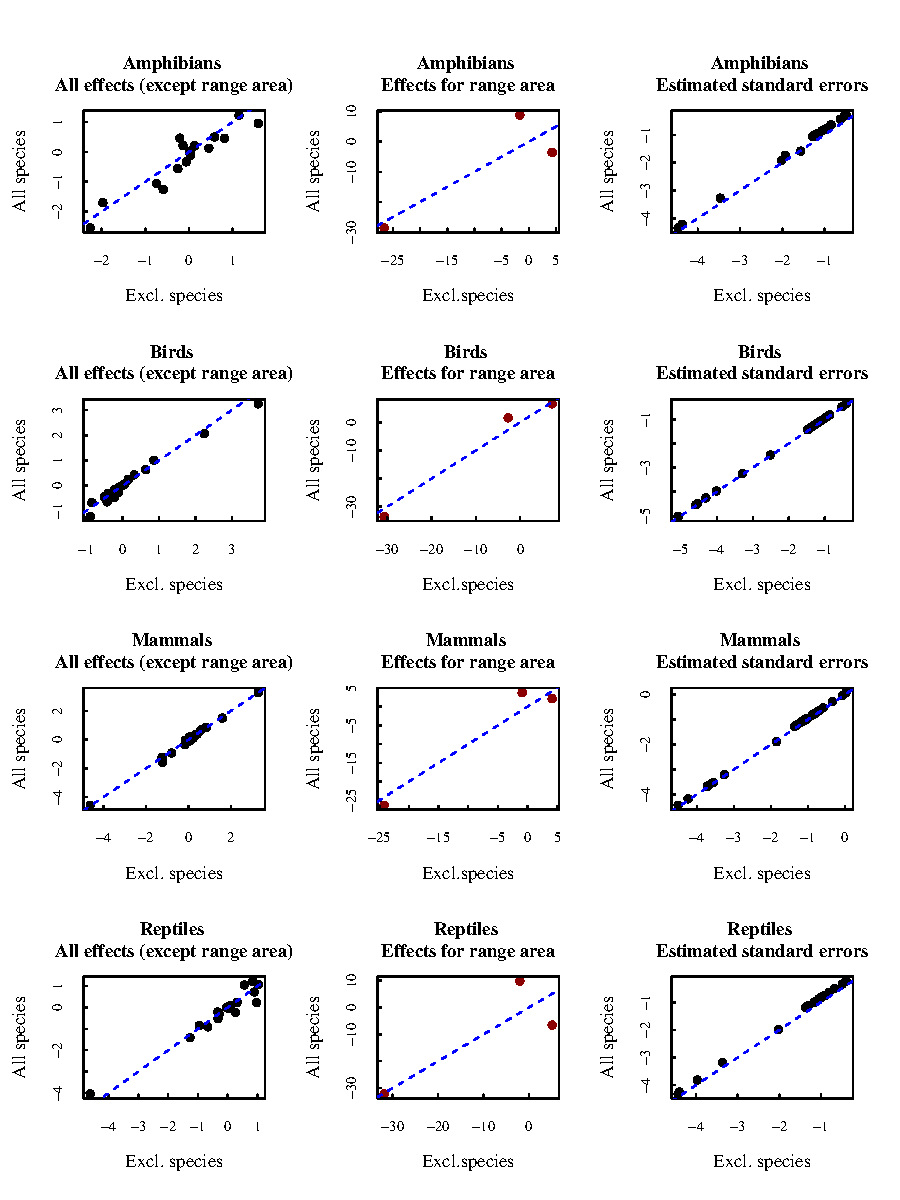
\includegraphics[scale=0.85, trim={0 0 5.5cm 0}, clip]{Supporting/Chapter4/Figures/ClimateChangeModelsEstimates.pdf}
\caption[Effects for the PGLS models investigating associations between species-level ecological characteristics and climate-change sensitivity, either fitted on all species (y--axis), or fitted on the species whose range area was $>$100 km$^2$ (x--axis)]{\textbf{Effects for the PGLS models investigating associations between species-level ecological characteristics and climate-change sensitivity}, either fitted on all species (y--axis), or fitted on the species whose range area was $>$100 km$^2$ (x--axis). Overall, the estimates from both sets of models were congruent, except for those estimated for geographical range area (I show the effects for range area separately from the effects of other characteristics). Across all classes, the relationship between sensitivity and geographical range area was reversed between the two sets of models. I found that sensitivity was positively associated with geographical range area when including all species, likely because of the underestimation of climate-change sensitivity for the most narrow-ranging species when working with a resolution of 5 km$^2$ (see Figure \ref{SI_4_Figure7}). The dashed line is the identity line (y=x).}
\label{SI_4_Figure22}
\end{figure}


%% ROBUSTNESS to the exclusion of migratory species

\begin{figure}[h!]
\centering
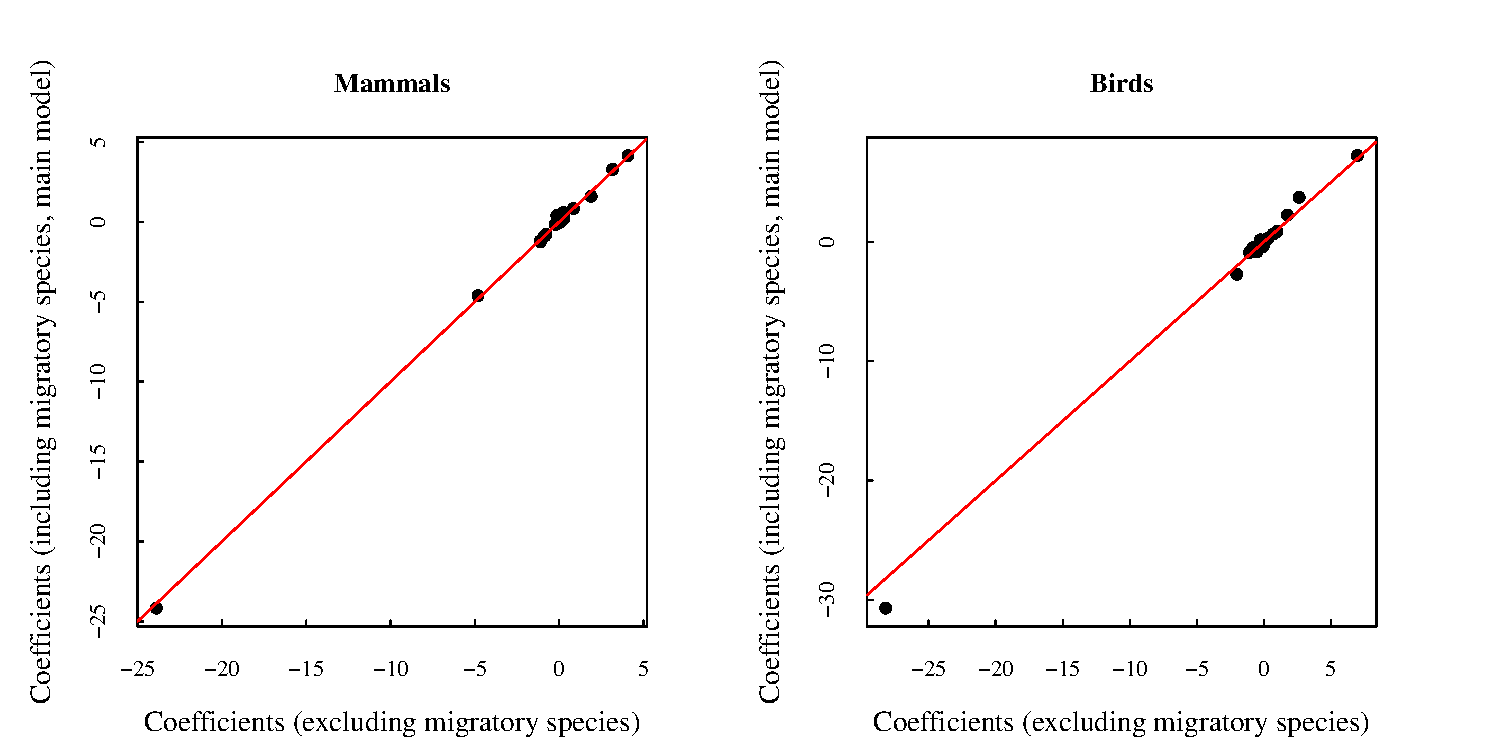
\includegraphics[scale=0.7, clip]{Supporting/Chapter4/Figures/Migratory_species_excluded/coefficients.pdf}
\caption[Effects for the PGLS models investigating associations between species-level ecological characteristics and climate-change sensitivity, either fitted on all birds and mammals (y--axis), or on the subset of bird and mammal species that were found not to be migratory (x--axis)]{\textbf{Effects for the PGLS models investigating associations between species-level ecological characteristics and climate-change sensitivity,} either fitted on all birds and mammals (y--axis), or on the subset of bird and mammal species that were found not to be migratory (x--axis). Overall, the estimates from both sets of models were congruent. The dashed line is the identity line (y=x).}
\label{SI_4_migratory_coefs}
\end{figure}

\begin{figure}[h!]
\centering
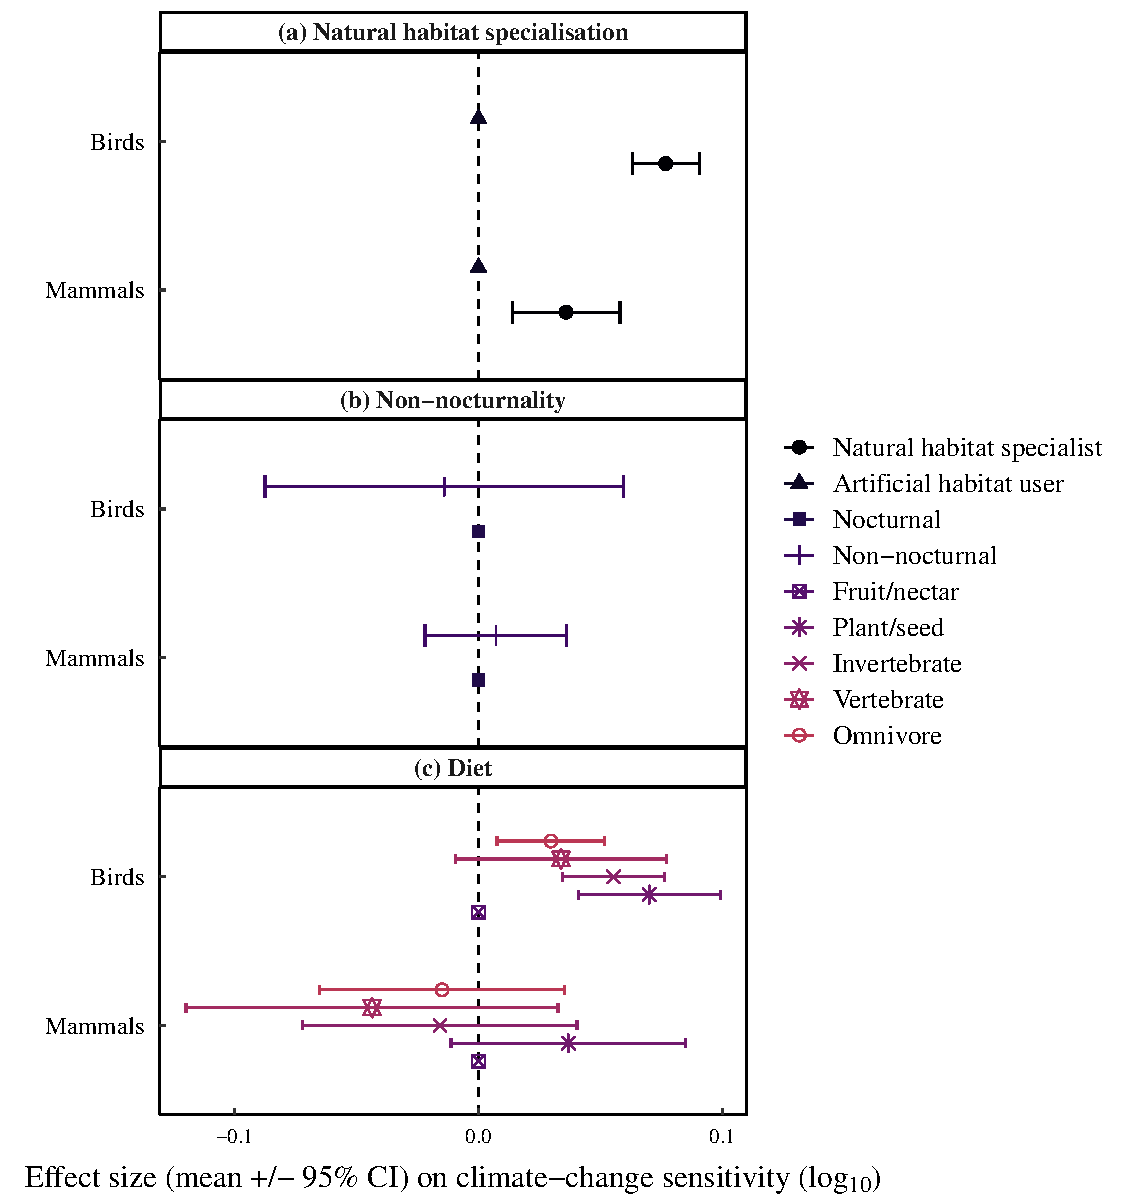
\includegraphics[scale=0.8, clip]{Supporting/Chapter4/Figures/Migratory_species_excluded/ExcludeMigratory_FigureCategorical.pdf}
\caption[Estimated effects of the categorical traits on climate-change sensitivity, from the PGLS models fitted on birds and mammals, excluding species identified as migratory]{\textbf{Estimated effects of the categorical traits on climate-change sensitivity, from the PGLS models fitted on birds and mammals, excluding species identified as migratory (mean effect $\pm$95\% confidence interval).} For each categorical trait, I show the effect size for all levels referring to the reference level (vertical dashed line). \textbf{(a)} For artificial habitat use, the reference level is `Artificial habitat user'; \textbf{(b)} for diel activity, the reference level is `Nocturnal'; \textbf{(c)} for diet, the reference level (for mammals and birds) is `Fruit/nectar' eaters. }
\label{SI_4_migratory_cat}
\end{figure}

\begin{figure}[h!]
\centering
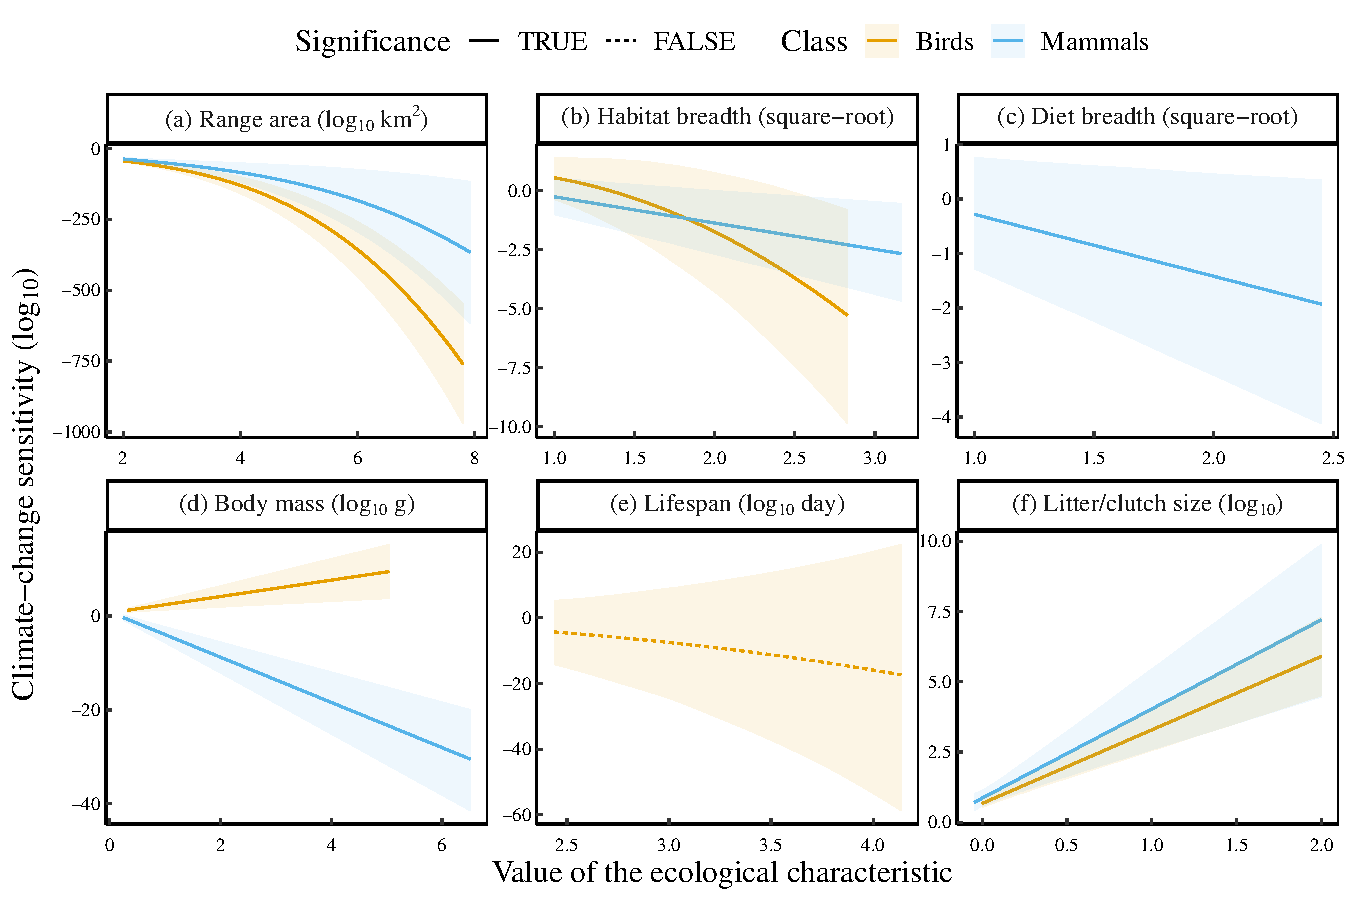
\includegraphics[scale=0.8, clip]{Supporting/Chapter4/Figures/Migratory_species_excluded/ExcludeMigratory_FigureContinuous.pdf}
\caption[Effects of the continuous ecological characteristics on climate-change sensitivity, estimated from the PGLS models fitted on birds and mammals, excluding species identified as migratory]{\textbf{Effects of the continuous ecological characteristics on climate-change sensitivity, estimated from the PGLS models fitted on birds and mammals, excluding species identified as migratory.} The lines represent the estimated relationships between climate-change sensitivity and ecological characteristics; the shaded areas are 95\% confidence intervals.}
\label{SI_4_migratory_cont}
\end{figure}

\clearpage
\section{Validations on complete trait data subsets}

%% Synthesis table
\begin{landscape}
%\subsection{Synthesis table}
\label{SI_4_Table22}
\begin{table}
\centering
\caption[Summary of the effects of the ecological characteristics (except for diet) on (a) species' responses to disturbed land uses (`within land-use type' effects) and (b) species climate-change sensitivity, for each class of terrestrial vertebrates, from validation models using empirical, non imputed trait values]{\textbf{Summary of the effects of the ecological characteristics (except for diet) on (a) species' responses to disturbed land uses (`within land-use type' effects) and (b) species climate-change sensitivity, for each class of terrestrial vertebrates, \textit{from the models fitted on empirical trait values (excluding all imputed values)}.} The symbol \colorbox{Salmon}{\textcolor{BrickRed}{\textbf{--}}} indicates where a characteristic has a significant negative effect on occurrence probability within a disturbed land-use type (within any of the land-use intensities), or where the characteristic renders species significantly more sensitive to climate change. A \colorbox{YellowGreen}{\textcolor{ForestGreen}{\textbf{+}}} indicates a significantly positive effect of a characteristic on occurrence probability in a land-use type (within any of the land-use intensities), or significantly lower sensitivity to climate change. For the land-use effects, I report `within land-use type effects' here, that is, within a disturbed land use whether there were significant differences in occurrence probability among species with different trait values. These effects were derived from the interactive terms of the full models.}
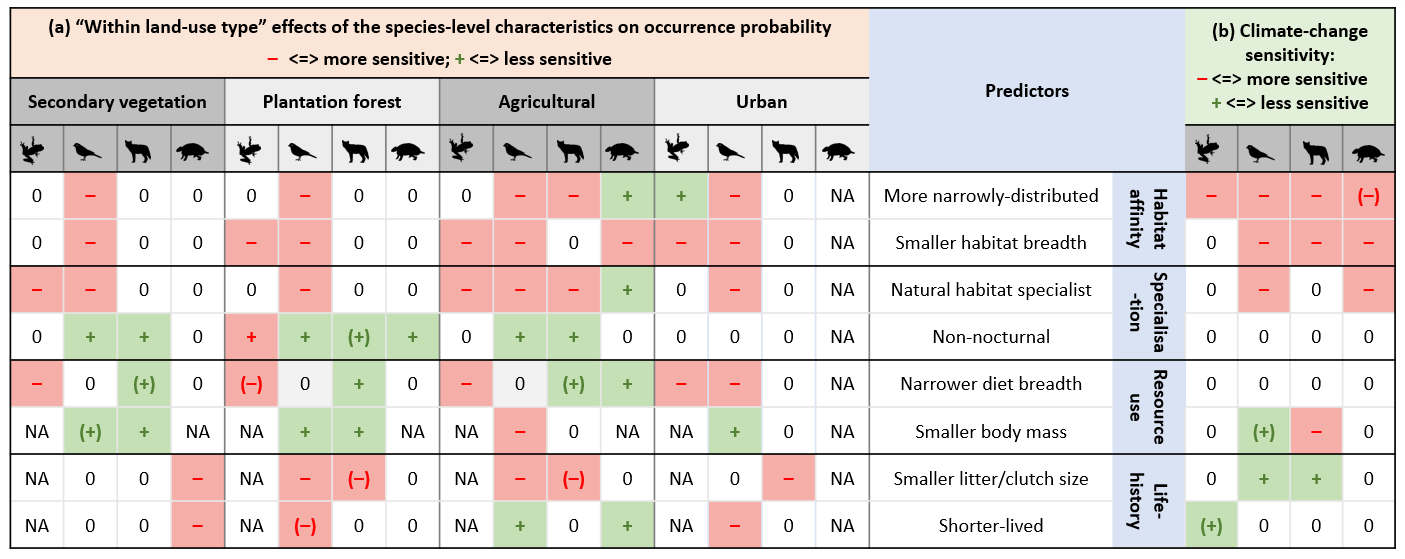
\includegraphics[scale=0.8]{Supporting/Chapter4/Figures/SynthesisTableValidation2}
\end{table}
\end{landscape}

\begin{comment}
\begin{figure}[h!]
\centering
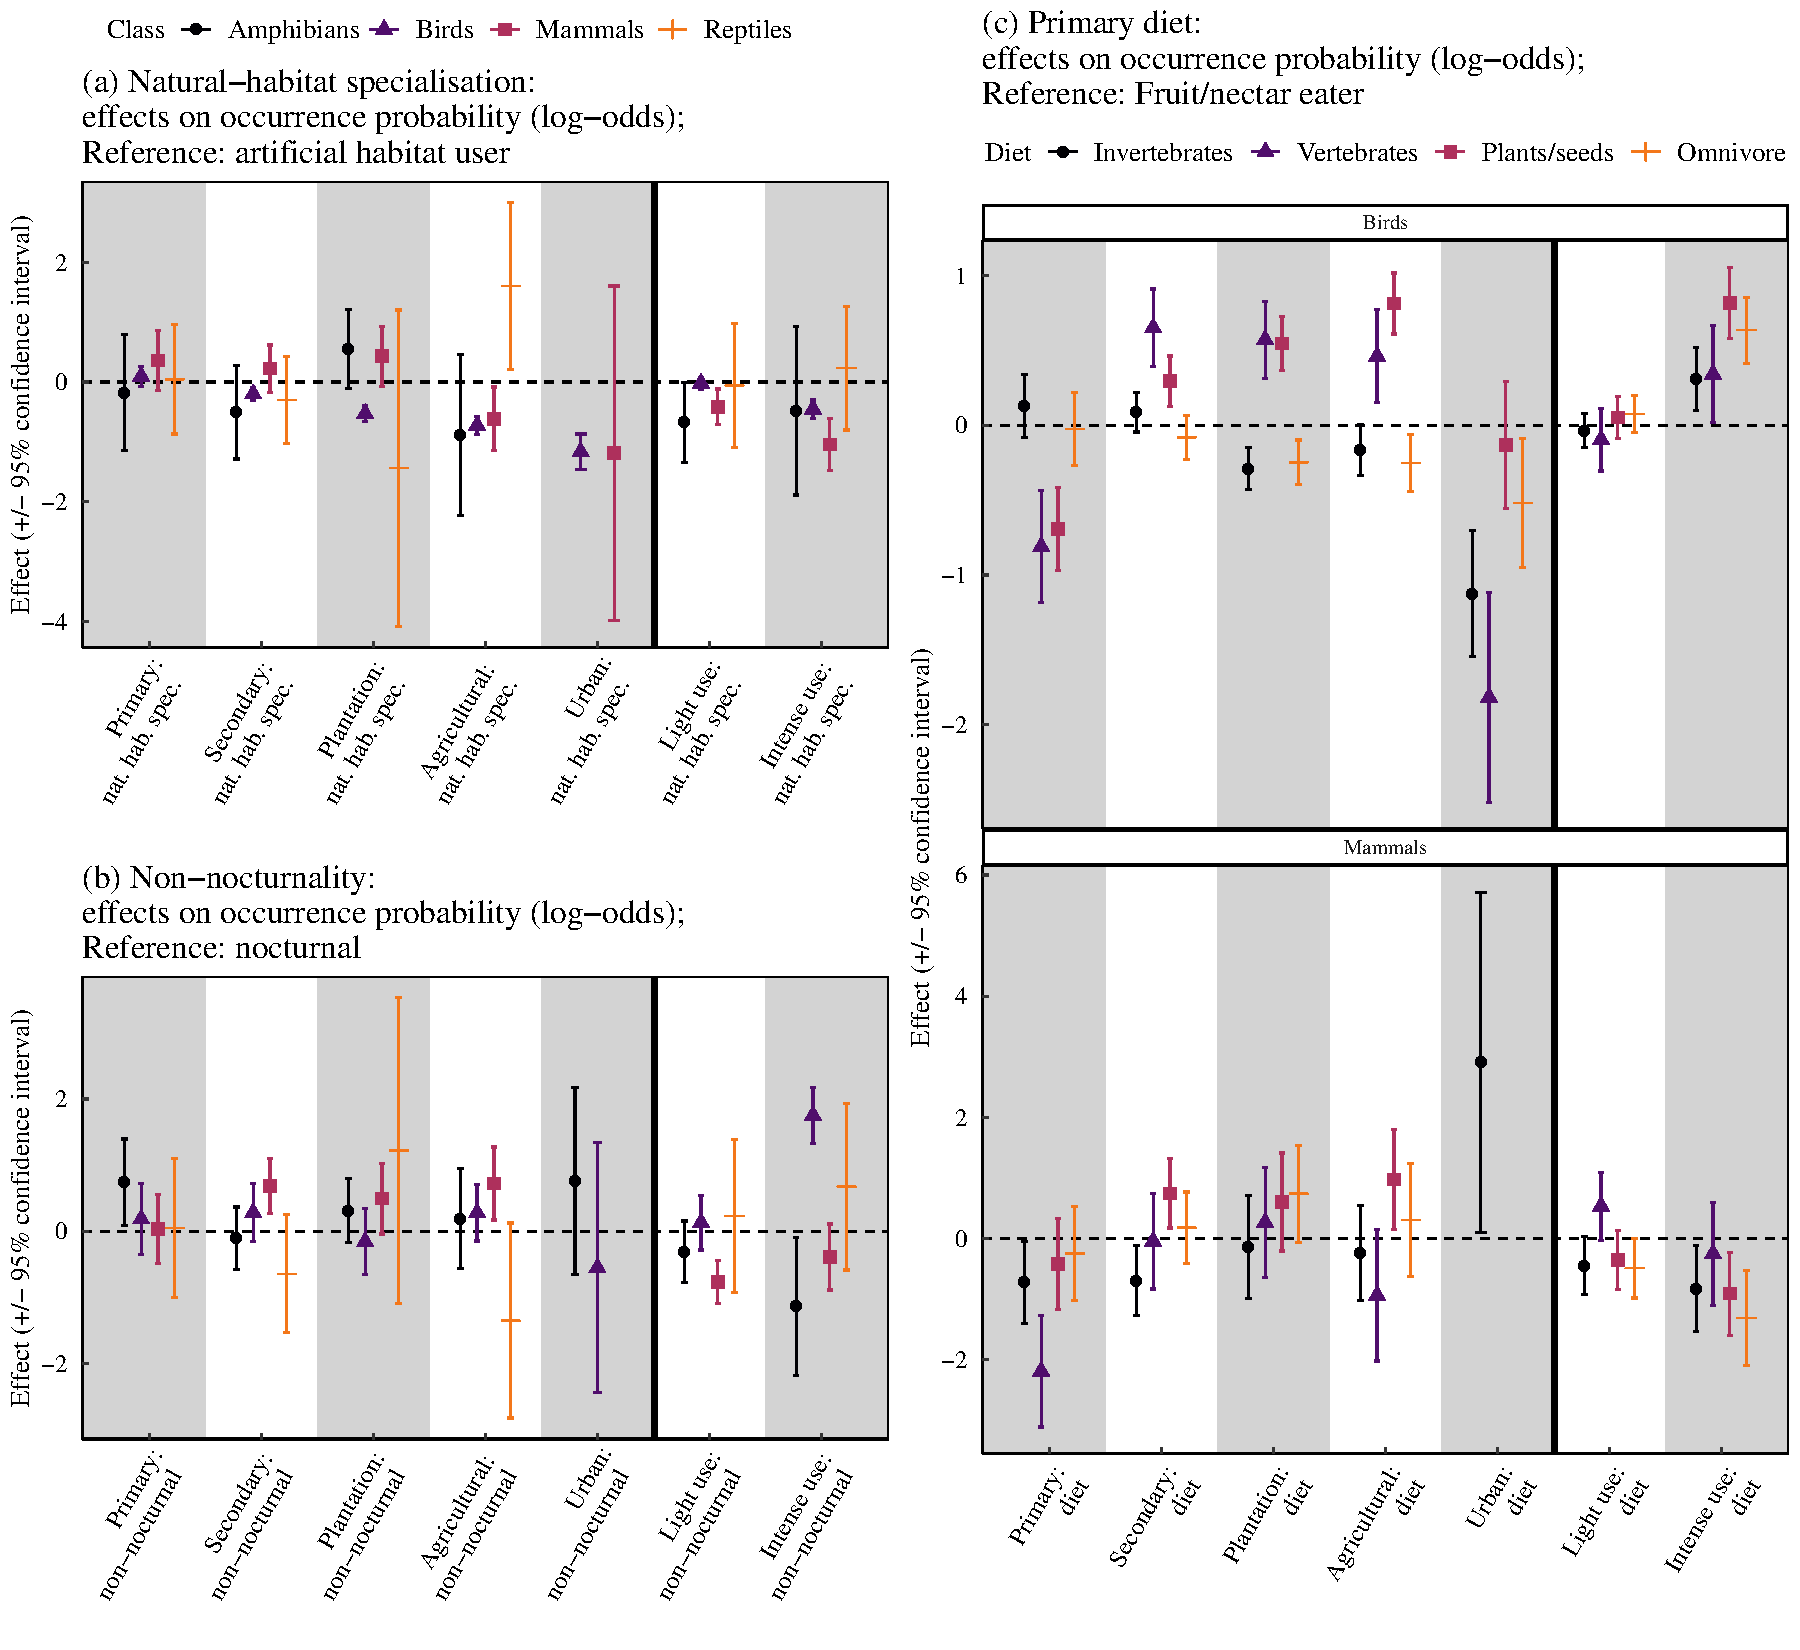
\includegraphics[scale=0.6]{Supporting/Chapter4/Figures/Land_use_categorical_traits_validation}
\caption[]{}
\label{}
\end{figure}
\end{comment}

%\subsection{Predicted occurrence probability as a function of land use, land-use intensity, diet and their interactions, in each class (validation on empirical trait data subsets (excluding imputed trait values) using partial models)}

\begin{figure}[h!]
\centering
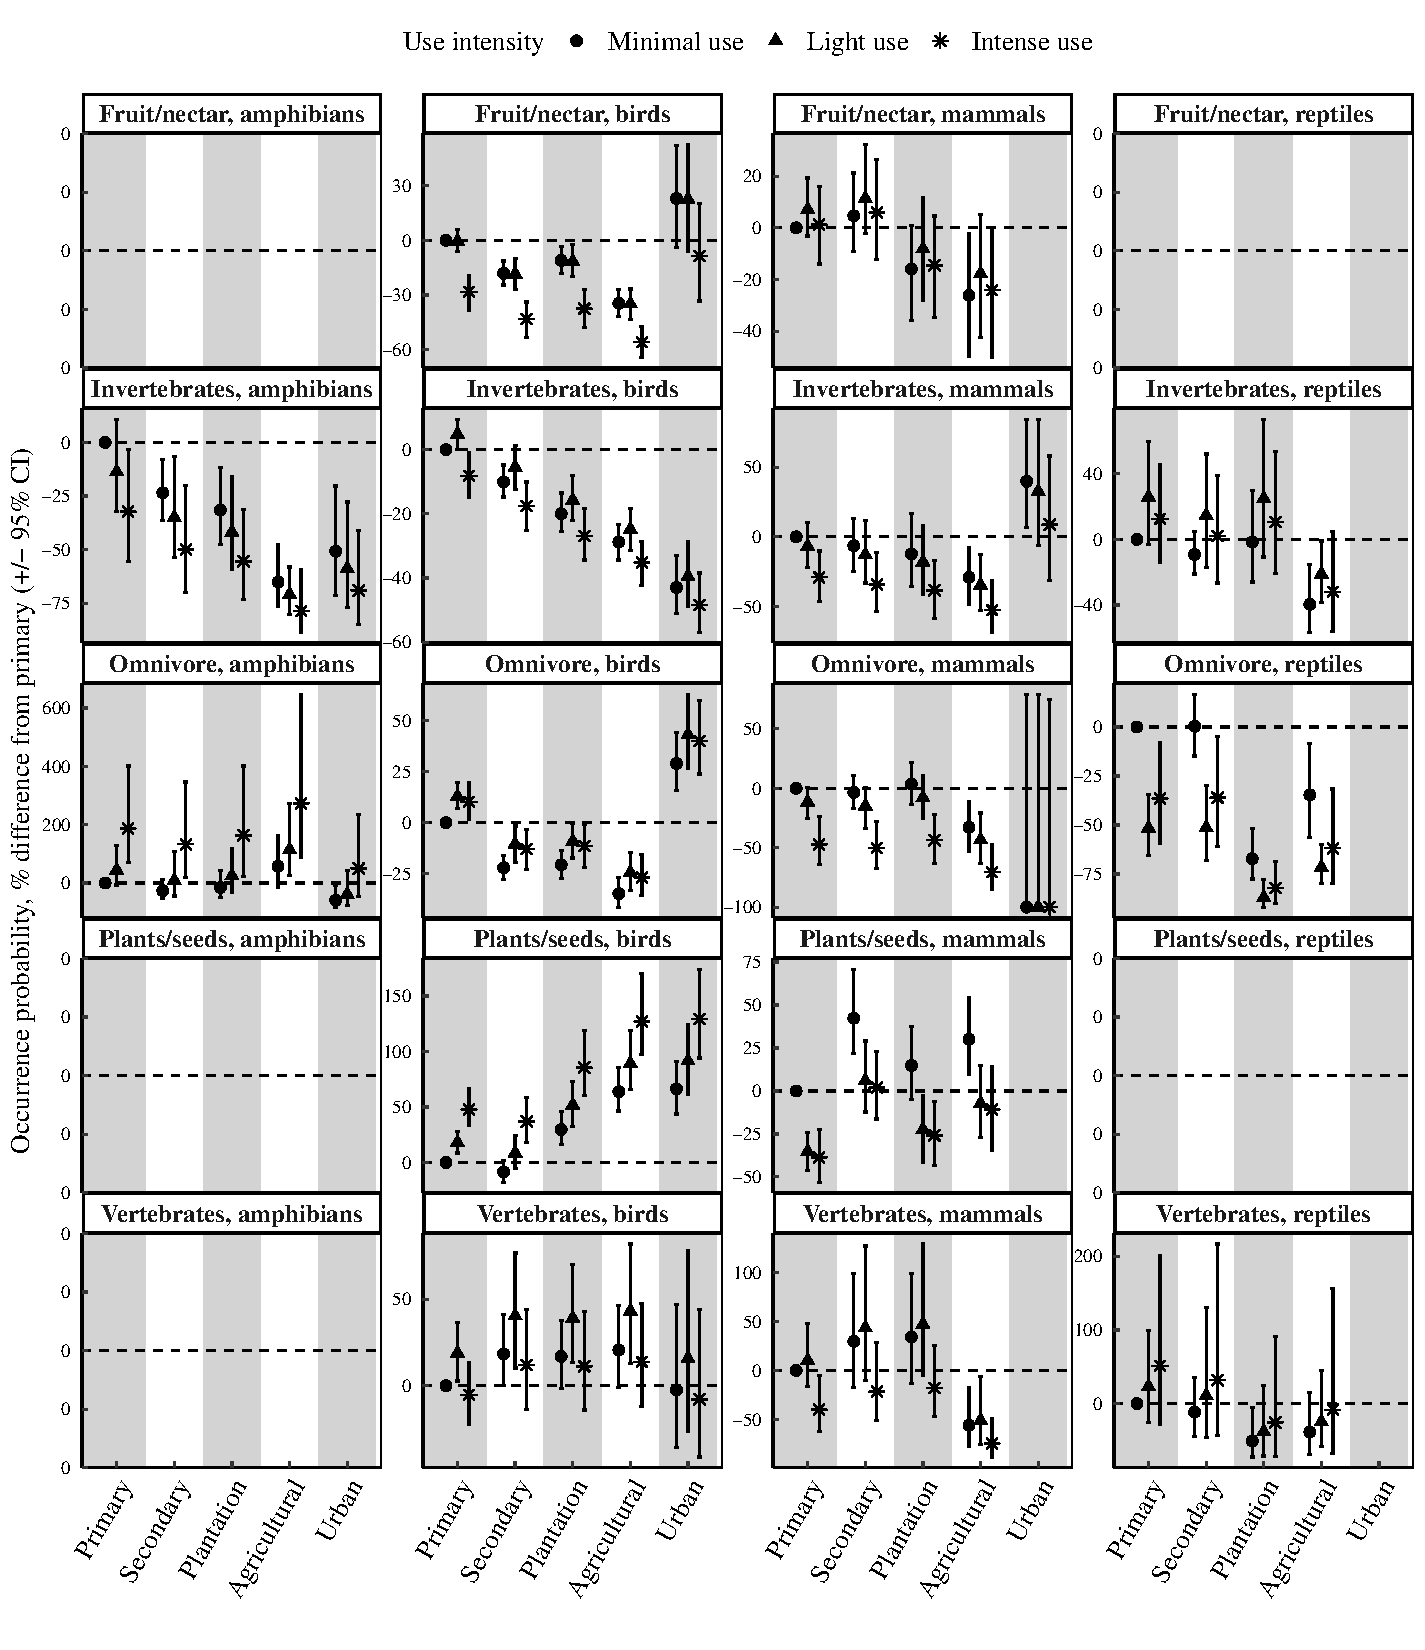
\includegraphics[scale=0.65]{Supporting/Chapter4/Figures/Partial_models_predictions/Validations/Diet}
\caption[Predicted occurrence probability as a function of land use, land-use intensity, diet and their interactions in each class: from validation models using empirical, non imputed trait values]{\textbf{Predicted occurrence probability as a function of land use, land-use intensity, diet and their interactions in each class. The predictions were obtained from the partial models fitted in each class for diet, \textit{estimated using empirical trait data subsets (i.e., excluding imputed trait values)}}. Empty plots are drawn where there were no data for a diet category in a given class (e.g., amphibian fruit/nectar eaters). Effects could not be estimated for urban reptiles, as well as for urban vertebrate, fruit/nectar and plant/seed eaters for mammals because there were no sampled species. The predictions are rescaled with reference to minimally-used primary vegetation. Primary: primary vegetation; Secondary: secondary vegetation; plantation: plantation forest; agricultural: cropland and pasture.}
\label{SI_4_Figure23}
\end{figure}


\begin{comment}

%\clearpage

%\subsection{PGLS models: validations on empirical trait data subsets}

%% PGLS model summaries - validation -- amphibians

\begin{table}[!h] 
\renewcommand{\baselinestretch}{1}
\renewcommand{\arraystretch}{1}
\begin{center}\fontsize{9}{11}\selectfont  
  \caption[Summary for the PGLS model fitted on amphibians: validations using the empirical trait data subset]{\textbf{Summary for the PGLS model fitted on amphibians, \textit{using the empirical trait data subset (i.e., excluding imputed trait values)}}, looking at the association between the species-level ecological characteristics and climate-change sensitivity.} 
  \label{SI_4_Table23} 
\begin{tabular}{@{\extracolsep{5pt}} ccccc} 
\\[-1.8ex]\hline 
\hline \\[-1.8ex] 
 & Estimate & Std. Error & t value & Pr(\textgreater \textbar t\textbar ) \\ 
\hline \\[-1.8ex] 
Intercept & $1.825$ & $0.342$ & $5.344$ & $<0.001$ \\ 
log$_{10}$(Body mass) & $$-$0.030$ & $0.035$ & $$-$0.875$ & $0.385$ \\ 
log$_{10}$(Lifespan proxy) & $0.180$ & $0.103$ & $1.742$ & $0.086$ \\ 
log$_{10}$(Litter/clutch size) & $0.052$ & $0.032$ & $1.639$ & $0.106$ \\ 
log$_{10}$(Range area) & $$-$0.261$ & $0.024$ & $$-$10.888$ & $<0.001$ \\ 
square-root(Habitat breadth) & $$-$0.032$ & $0.030$ & $$-$1.078$ & $0.285$ \\ 
square-root(Diet breadth) & $$-$0.068$ & $0.107$ & $$-$0.635$ & $0.527$ \\ 
Specialisation: Natural habitat specialist & $$-$0.006$ & $0.059$ & $$-$0.095$ & $0.925$ \\ 
Diel activity: Non-nocturnal & $$-$0.009$ & $0.044$ & $$-$0.205$ & $0.839$ \\ 
\hline \\[-1.8ex] 
\end{tabular} 
\end{center}
\end{table} 

%% PGLS model summaries - validation -- birds

\begin{table}[!h] 
\renewcommand{\baselinestretch}{1}
\renewcommand{\arraystretch}{1}
\begin{center}\fontsize{9}{11}\selectfont 
  \caption[Summary for the PGLS model fitted on birds: validations using the empirical trait data subset]{\textbf{Summary for the PGLS model fitted on birds, \textit{using the empirical trait data subset (i.e, excluding imputed traits values)}}, looking at the association between the species-level ecological characteristics and climate-change sensitivity.} 
  \label{SI_4_Table24} 
\begin{tabular}{@{\extracolsep{5pt}} ccccc} 
\\[-1.8ex]\hline 
\hline \\[-1.8ex] 
 & Estimate & Std. Error & t value & Pr(\textgreater \textbar t\textbar ) \\ 
\hline \\[-1.8ex] 
Intercept & $1.551$ & $0.143$ & $10.875$ & $<0.001$ \\ 
log$_{10}$(Body mass) & $0.020$ & $0.011$ & $1.759$ & $0.079$ \\ 
log$_{10}$(Lifespan proxy) & $0.047$ & $0.036$ & $1.308$ & $0.191$ \\ 
log$_{10}$(Litter/clutch size) & $0.212$ & $0.022$ & $9.487$ & $<0.001$ \\ 
log$_{10}$(Range area) & $$-$0.230$ & $0.003$ & $$-$73.130$ & $<0.001$ \\ 
square-root(Habitat breadth) & $$-$0.011$ & $0.005$ & $$-$2.319$ & $0.020$ \\ 
square-root(Diet breadth) & $0.015$ & $0.011$ & $1.319$ & $0.187$ \\ 
Specialisation: Natural habitat specialist & $0.044$ & $0.007$ & $6.586$ & $<0.001$ \\ 
Diel activity: Non-nocturnal & $0.001$ & $0.058$ & $0.019$ & $0.984$ \\ 
Primary diet: Invertebrates & $0.047$ & $0.014$ & $3.330$ & $0.001$ \\ 
Primary diet: Omnivore & $0.016$ & $0.014$ & $1.144$ & $0.253$ \\ 
Primary diet: Plants/seeds & $0.048$ & $0.016$ & $2.993$ & $0.003$ \\ 
Primary diet: Vertebrates & $$-$0.005$ & $0.022$ & $$-$0.247$ & $0.805$ \\ 
\hline \\[-1.8ex] 
\end{tabular} 
\end{center}
\end{table} 


%% PGLS model summaries - validation -- mammals
\begin{table}[!h]
\renewcommand{\baselinestretch}{1}
\renewcommand{\arraystretch}{1}
\begin{center}\fontsize{9}{11}\selectfont 
  \caption[Summary for the PGLS model fitted on mammals: validations using the empirical trait data subset]{\textbf{Summary for the PGLS model fitted on mammals, \textit{using the empirical trait data subset (i.e., excluding imputed trait values)}}, looking at the association between the species-level ecological characteristics and climate-change sensitivity.} 
  \label{SI_4_Table25} 
\begin{tabular}{@{\extracolsep{5pt}} ccccc} 
\\[-1.8ex]\hline 
\hline \\[-1.8ex] 
 & Estimate & Std. Error & t value & Pr(\textgreater \textbar t\textbar ) \\ 
\hline \\[-1.8ex] 
Intercept & $2.194$ & $0.187$ & $11.705$ & $<0.001$ \\ 
log$_{10}$(Body mass) & $$-$0.047$ & $0.012$ & $$-$3.865$ & $<0.001$ \\ 
log$_{10}$(Lifespan proxy) & $0.065$ & $0.046$ & $1.416$ & $0.157$ \\ 
log$_{10}$(Litter/clutch size) & $0.147$ & $0.034$ & $4.293$ & $<0.001$ \\ 
log$_{10}$(Range area) & $$-$0.269$ & $0.005$ & $$-$54.621$ & $<0.001$ \\ 
square-root(Habitat breadth) & $$-$0.042$ & $0.010$ & $$-$4.320$ & $<0.001$ \\ 
square-root(Diet breadth) & $$-$0.030$ & $0.020$ & $$-$1.487$ & $0.137$ \\ 
Specialisation: Natural habitat specialist & $0.016$ & $0.013$ & $1.235$ & $0.217$ \\ 
Diel activity: Non-nocturnal & $0.012$ & $0.015$ & $0.792$ & $0.428$ \\ 
Primary diet: Invertebrates & $$-$0.038$ & $0.031$ & $$-$1.220$ & $0.223$ \\ 
Primary diet: Omnivores & $$-$0.031$ & $0.027$ & $$-$1.148$ & $0.251$ \\ 
Primary diet: Plants/seeds & $0.034$ & $0.027$ & $1.298$ & $0.195$ \\ 
Primary diet: Vertebrates & $$-$0.039$ & $0.040$ & $$-$0.995$ & $0.320$ \\ 
\hline \\[-1.8ex] 
\end{tabular}
\end{center} 
\end{table} 

%% PGLS model summaries - validation -- reptiles


\begin{table}[!h]
\renewcommand{\baselinestretch}{1}
\renewcommand{\arraystretch}{1}
\begin{center}\fontsize{9}{11}\selectfont 
  \caption[Summary for the PGLS model fitted on reptiles: validations using the empirical trait data subset]{\textbf{Summary for the PGLS model fitted on reptiles, \textit{using the empirical trait data subset (i.e., excluding imputed trait values)}}, looking at the association between the species-level ecological characteristics and climate-change sensitivity.} 
  \label{SI_4_Table26} 
\begin{tabular}{@{\extracolsep{5pt}} ccccc} 
\\[-1.8ex]\hline 
\hline \\[-1.8ex] 
 & Estimate & Std. Error & t value & Pr(\textgreater \textbar t\textbar ) \\ 
\hline \\[-1.8ex] 
Intercept & $1.269$ & $0.522$ & $2.433$ & $0.018$ \\ 
log$_{10}$(Body mass) & $$-$0.033$ & $0.058$ & $$-$0.570$ & $0.571$ \\ 
log$_{10}$(Lifespan proxy) & $0.015$ & $0.130$ & $0.119$ & $0.905$ \\ 
log$_{10}$(Litter/clutch size) & $0.095$ & $0.128$ & $0.739$ & $0.463$ \\ 
log$_{10}$(Range area) & $$-$0.093$ & $0.049$ & $$-$1.878$ & $0.066$ \\ 
square-root(Habitat breadth) & $$-$0.094$ & $0.045$ & $$-$2.097$ & $0.041$ \\ 
square-root(Diet breadth) & $0.067$ & $0.112$ & $0.595$ & $0.554$ \\ 
Specialisation: Natural habitat specialist & $0.221$ & $0.075$ & $2.936$ & $0.005$ \\ 
Diel activity: Non-nocturnal & $$-$0.118$ & $0.080$ & $$-$1.486$ & $0.143$ \\ 
\hline \\[-1.8ex] 
\end{tabular} 
\end{center}
\end{table} 

\end{comment}


\clearpage
